 %================================================================================
% Erstellt am: 		10.07.2008
% Überarbeitet am:	08.07.2009
% Autor:			Holger Fischer
%
% Kann frei für Bachelor-/Diplom-/Masterarbeiten verwendet werden.
% Viel Erfolg!!!
%================================================================================

%Einbinden der Datei header.tex; diese enthält alle verwendeten Pakete,
%sowie Änderungen am Layout
%!TEX root = ../Dokumentation.tex

%Da Latex für englischsprachige Texte ausgerichtet ist,
%wird als Dokumentenklasse das "`scrbook"' von Markus Kohm verwendet.
%Dieses ist für deutschsprachige Texte ausgelegt.
%BCOR12mm: 12mm Bindekorrektur (Verbreiterung des linken Randes)
%DIV11: entspricht in etwas der geforderten Textgröße und Seitenränder
%titlepage: eine Titelseite wird verwendet
%a4paper: DIN A4
%oneside: für eine spätere einseitige Bedruckung
%Original: \documentclass[BCOR12mm,DIV11,titlepage,a4paper,oneside]{scrbook}
\documentclass[DIV11,titlepage,a4paper,oneside,10pt]{scrbook}

\textheight = 23cm

%Paket für deutsche Silbentrennung etc.
\usepackage{ngerman}

%Paket für Zeichenkodierung, entspricht UTF-8
\usepackage[utf8x]{inputenc}

%Paket das die Ausgabefonts definiert
\usepackage[T1]{fontenc}

%Paket für das Einbinden von Grafiken über die figure-Umgebung
\usepackage{graphicx}

%Paket zum Ändern der Listenabstände
\usepackage{enumitem}
\setlist[itemize]{itemsep=0mm}
\setlist[enumerate]{itemsep=0mm}

%Paket zum Ändern der Kopf- und Fußzeile
\usepackage{fancyhdr}

%fancypagestyle{fancy}
\renewcommand{\headrulewidth}{0pt}
\fancyhf{}
%\fancyfoot[L]{FANCY}
\fancyfoot[R]{\thepage}

\fancypagestyle{plain}{
	\renewcommand{\headrulewidth}{0pt}
	\fancyhf{}
%	\fancyfoot[L]{PLAIN}
	\fancyfoot[R]{\thepage}
}

\pagestyle{plain}

%Abbildungsnummerierung ändern (abhängig von chapter, z.B. Abbildung 1.1)
\renewcommand*{\thefigure}{\thechapter.\arabic{figure}}
%Tabellennummerierung ändern (abhängig von chapter, z.B. Tabelle 1.1)
\renewcommand*{\thetable}{\thechapter.\arabic{table}}

%Paket, um ein Glossar/Abkürzungsverzeichnis anzulegen
\usepackage{nomencl}
\let\abbrev\nomenclature
%Der Name wird in Glossar geändert
\renewcommand{\nomname}{Glossar (optional)}
%Definiert die Aufteilung im Glossar zwischen Begriffen und Erläuterung
\setlength{\nomlabelwidth}{.25\hsize}
%Definiert die Punktelinien im Glossar
\renewcommand{\nomlabel}[1]{#1 \dotfill}
\setlength{\nomitemsep}{-\parsep}
%Veranlasst die Erstellung des Glossars
\makenomenclature

%Einrückungen nach Absätzen und Grafiken verhindern
\setlength{\parindent}{0pt}

%Verhindern, dass eine neue Seite für ein einzelnes Wort/Zeile verwendet wird
\clubpenalty = 10000 % schliesst Schusterjungen aus
\widowpenalty = 10000 % schliesst Hurenkinder aus (keine Beleidigung, sondern wirklich ein Fachbegriff)

%Paket für ein deutsches Literaturverzeichnis
\usepackage{bibgerm}

%Paket für die Verwendung von URLs durch den Befehl \url{}
\usepackage{url}

%Paket für Zeilenabstand (onehalfspace, singlespace)
\usepackage{setspace}

%Paket zur Erzeugung von Anführungszeichen durch \enquote{Text}
\usepackage[ngerman]{babel}
\usepackage[babel, german=quotes]{csquotes}

%Paket für farbigen Text
%black,white,green,red,blue,yellow,cyan,magenta
\usepackage{color}

%Paket für farbigen Hintergrund für Verbatim-Umgebung (Quelltext-Umgebung)
\usepackage{fancyvrb}
\usepackage{verbatim,moreverb}

%Grauton für Quelltext-Umgebung definieren 80% Grau
\definecolor{source}{gray}{0.95}

%Paket für Quelltext-Umgebung
\usepackage{listings}

%Paket für Positionierung der Objekte ohne Float (Verwendungsbsp.: \begin{figure}[H])
\usepackage{float}

%Paket für Tabellen über die gesamte Breite
\usepackage{tabularx}

%Paket für Definitionen, etc.
\usepackage{amsthm}

%Paket zur Erzeugung von Hyperrefs und PDF Informationen
\usepackage[pdftex,plainpages=false,pdfpagelabels,
            pdftitle={Projektdokumentation},
            pdfauthor={Dennis Meyer, Dominik Schilling}
            ]{hyperref}


% ###################
% Eigene Änderungen

\usepackage{subfig}
\usepackage{wrapfig}

% Codestyling
\definecolor{darkgreen}{rgb}{0,0.5,0}
\lstset{
    breaklines		= true,
    numbers			= left,
    stepnumber		= 1,
    basicstyle		= \ttfamily,
    numberstyle		= \footnotesize\ttfamily,
    backgroundcolor	= \color{source},
    language		= java,
    commentstyle    = \color{darkgreen}\ttfamily,
    keywordstyle    = \color{blue}\ttfamily,
    stringstyle		= \color{red},
    showspaces      = false,
    showstringspaces= false,
    captionpos		= b,
    frame			= single,
    aboveskip		= 1cm,
    belowskip		= 1cm,
}
\renewcommand\lstlistingname{Code}
\renewcommand\lstlistlistingname{Codeverzeichnis}


\begin{document}

%=== Einleitung ======================================================
%Seitennummerierung Abstract bis einschließlich Inhaltsverzeichnis
\frontmatter

%Einbinden der Titelseite
%!TEX root = ../dokumentation.tex

\begin{titlepage}

\begin{center}

%Logo der Fachhochschule Köln
\begin{figure}[!ht]
	\centering
		
\includegraphics[natwidth=920pt, natheight=95pt, width=1.0\textwidth]{inc/logoheader.pdf}
\end{figure}

\vspace{4.0cm}

\begin{Huge}
	\textbf{Entwicklungsprojekt }\\
	\vspace{0.1cm}
	\textbf{interaktive Systeme}\\

\end{Huge}

\vspace{0.8cm}

\begin{LARGE}
	\textbf{Find your Camp}\\
	\vspace{0.2cm}
	Dokumentation über ein verteiltes System\\
	\vspace{0.1cm}
	zum Mieten und Verleihen von \\
	\vspace{0.1cm}
	privaten Grundstücken als Campingplatz\\
\end{LARGE}

\vspace{2cm}

\begin{tabular}{rl}
        Dozent:  &  Prof. Dr. Kristian Fischer\\
       		 	 &  Prof. Dr. Gerhard Hartmann\\
       			 &  \small Fachhochschule Köln \\[1.0em]
      Betreuer:  &  David Bellingroth\\
				 &  Julian Rahe\\
       			 &  \small Fachhochschule Köln\\
\end{tabular}

\vspace{1.6cm}

\begin{large}
	ausgearbeitet von\\
	\vspace{0.2cm}
\end{large}

\begin{Large}
	Dennis Meyer, Matrikelnr. 11084479\\
	Dominik Schilling, Matrikelnr. 11081691\\
	\vspace{1cm}
	Wintersemester 2013/2014
\end{Large}

\end{center}

\end{titlepage}


%Zeilenabstand für das Inhaltsverzeichnis 1 fach
\singlespacing
%Einbinden des Inhaltsverzeichnis
%!TEX root = ../dokumentation.tex

\cleardoublepage
\pagenumbering{gobble}
\tableofcontents
\cleardoublepage
\pagenumbering{arabic}


%Zeilenabstand für den Hauptteil ist 1,5 fach
\onehalfspacing

%=== Hauptteil =======================================================
%Seitennummerierung des Hauptteils
\mainmatter
	%Die Zähler für Tabellen und Abbildungen werden zurückgesetzt, damit
	%in jedem Kapitel die Nummerierung neu beginnt
	\setcounter{table}{1}
	\setcounter{figure}{1}
	%Einbinden des ersten Kapitels

	%Einführung
	%!TEX root = ../dokumentation.tex

\chapter{Einführung}
"Im Rahmen des Moduls Entwicklungsprojekt interaktive Systeme, geht es um die Konzipierung und Umsetzung einer verteilten, multimedialen Anwendung unter Verwendung zuvor erlernter Grundlagen. Innerhalb des Projektes sollen Methoden und Techniken der Veranstaltungen der Mensch Computer Interaktion und Web-basierte Anwendungen 2: Verteilte Systeme selbstständig geplant und durchgeführt werden."\footnote{Auszug der Konzepteinleitung, Seite 1}\\

Nach Ausarbeitung des Konzeptes innerhalb der ersten Projektphase, befasst sich diese Dokumentation mit der weiterführenden Projektarbeit bis hin zur finalen Abgabe der entstandenen Projektergebnisse.\\
Die bereits begonnene Auseinandersetzung mit wesentlichen Aspekten der Mensch Computer Interaktion und Webbasierte Anwendungen 2, wird weiter vertieft und gewonnene Ergebnisse dargelegt.\\

Die vorliegende Projektdokumentation ist strukturell in mehrere Teile aufgebaut.\\
Nach der allgemeinen Einführung folgt als erster Hauptbestandteil die Prozessdokumentation, die den zeitlichen Ablauf des Projektes fokusiert. 
Darin wird die Entwicklung nach Konzeptabgabe, einzelne Arbeitsschritte und angewendete MCI Methoden mit entstandenen Ergebnissen beschrieben.\\ Es folgt die Systemdokumentation, welche das entwickelte System genauer erklärt und die Alternativen und Abwägungen während der Entwicklungsphase herausstellt.\\ 
Der letzte Abschnitt ist die Installationsdokumentation, bei der die Anforderungen an ein System und dazugehörige Installationsschritte erläutert werden.\\

Die überarbeitete Version des Konzept befindet sich im Anhang dieses Dokuments und wird an gegebenen Stellen referenziert.



	%Die Zähler für Tabellen und Abbildungen werden zurückgesetzt, damit
	%in jedem Kapitel die Nummerierung neu beginnt
	\setcounter{table}{1}
	\setcounter{figure}{1}
 	%Einbinden des ersten Kapitels
	
	%Überarbeitungen des Konzeptes jetzt in Kapitel 3.1
	%%!TEX root = ../dokumentation.tex

\chapter{Überarbeitung des Konzeptes}





	%Die Zähler für Tabellen und Abbildungen werden zurückgesetzt, damit
	%in jedem Kapitel die Nummerierung neu beginnt
	\setcounter{table}{1}
	\setcounter{figure}{1}
	%Einbinden des zweiten Kapitels
	
	%Prozessdokumentation
	%!TEX root = ../dokumentation.tex

\chapter{Prozessdokumentation}

Zeitlicher Verlauf des Projektes\\
Schwierigkeiten/Probleme ⇒ Behebung/Umgang\\
Wichtige Entscheidungen\\
Beschreibung der durchgeführten MCI Methoden mit ihren Ergebnissen\\
Aktivitätenverteilung (Wer hat was gemacht?)\\
Projektplan (geplant ⇔ tatsächlich)\\
Ziel: nachvollziehbare Prozessqualität\\

\newpage

%!TEX root = ../dokumentation.tex

\section{Allgemeines}






\newpage

%!TEX root = ../dokumentation.tex

\section{Ausarbeitung MCI}

Was sind die Entwicklungsziele für das interaktive System? X\\
Wer sind die Benutzer? X\\
Was sind die user needs? X\\
Was sind die funktionalen und qualitativen Anforderungen; welche Rahmenbedingungen existieren? X\\
Welche organisatorischen Anforderungen liegen vor x\\
Wie soll methodisch im Projekt vorgegangen werden? Wie werden die beiden Perspektiven ("MMA" und "MCI") in EINEM Projekt systematisch und strukturiert berücksichtigt? Vorgehensmodelle? Begründung und kritische Diskussion der Alternativen notwendig. x\\
Welches sind die Aufgaben, welche Struktur weisen sie auf und in welchen Beziehungen stehen die Aufgaben zueinander?\\
Wie sieht ein valides Modell des Nutzungskontextes aus? x\\
Welche Metaphern und Paradigmen liegen in der Domäne vor?\\
Welches ist das konzeptuelle Modell für das präskriptive Aufgabenmodell? \\
Welche Bezüge existieren bzgl. der Entwicklungsziele?\\
Welche alternativen konzeptuellen Modelle wurden entwickelt und wie wurde mit Design-Alternativen verfahren?\\
Welche Interaktions-Paradigmen, -Modi und -Stile wurden in Betracht gezogen? Erörterung notwendig.\\
Welche Prototypen wurden entwickelt, was zeichnet die verschiedenen Prototypen-Alternativen aus und wie wurde eine Synthese der Alternativen erreicht?\\
Nach welchen Kriterien wurden die Evaluation-Methoden und -Techniken ausgewählt?\\
Welches sind die Evaluationsergebnisse, welchen Erfüllungsgrad der Entwicklungsziele weist der finale Prototyp auf?\\
Welche Konsequenzen für das Redesign ergeben sich?\\
Wie sehen die weiteren Iterationen aus?\\

\newpage

%!TEX root = ../dokumentation.tex

\section{Weiterführende Benutzermodellierung}
Innerhalb der Konzeptphase wurde bereits der Grundstein zur Benutzermodellierung gelegt. Bezogen auf die Zieldomäne fand eine Identifikation vorhandener Stakeholdergruppen samt Einordnung statt. Für die weitere Auseinandersetzung geht es nun darum, die einzelnen Benutzergruppen genauer zu analysieren und entsprechende User Profiles zu entwickeln, um die Anwender genauer bestimmten zu können. Daraufhin aufbauend sollen Beispielpersona erstellt werden, da diese innerhalb des Designprozesse geeigneter sind um Interaktionsprozesse nachvollziehbarer zu gestalten. Der Vorteil von Persona gegenüber User Profiles liegt darin, dass kognitive Vorgänge durch die “Modellierung” einer Person mit Hintergrundinformationen präziser zu erreichen sind. Zudem ist es während der Entwicklung (vorerst) nicht möglich mit realen Personen zusammen zu arbeiten. 

Auch wenn der Fokus des Usage Center Designs auf der eigentlichen Interaktion liegt, sollte diese Modellierungstiefe erreicht werden, da innerhalb des Verleihprozesses unterschiedliche Anwendertypen auftreten können mit eigenen (moralischen) Ansichten zum Shared Economy Konzept. Speziell bezogen auf eine Zielgruppe, die ihr Grundstück nur unter bestimmten Sicherheitsaspekten verleihen würde, kann die Auseinandersetzung neue Erkenntnisse zu geforderten Funktionalitäten und Restriktionen liefern.

\subsection{User Profiles}
Entsprechend der Stakeholderanalyse\footnote{Konzeptkapitel 3.1 Seite 14} und der genaueren Benutzerbetrachtung im Rahmen des Nutzungskontexts\footnote{Konzeptkapitel 3.2 Seite 18}, geht es im nächsten Detaillierungsgrad um die Entwicklung von User Profiles. Dabei werden entsprechend der Stakeholdergruppen charakterisierende Merkmale analysiert.\footnote{Entsprechend Draft zur MCI S.376}\\
Vorerst stellte sich die Frage, für welche Stakeholdergruppen die weitere Modellierung den größten Nutzen hat. Da innerhalb des Entwicklungsprozesses speziell auf die Bedürfnisse der Anwender eingegangen wird, erscheint es am sinnvollsten die Usergruppen zu betrachten, die direkt mit dem System agieren. Dazu zählen vorallem die primary und secundary user. Für die tertiären user, die in ihrer Funktion hauptsächlich als Interessenten oder Richtungsgeber tätig sind, soll dieser Schritt nicht im Detail durchgeführt werden. (Feedback abwarten) Als potentielle Stakeholder dieser Klasse wurden beispielsweise andere Unterkunftsanbieter oder die Stadt, als Interessent durch den Tourismus, identifiziert. Da diese Gruppen grundsätzlich eher konzeptioneller Natur sind, spielen sie für die Entwicklung keine tragende Rolle.\\

Zuerst werden die primary user untersucht. Dazu gehören die Reisenden als Mieter und die Grundstücksbesitzer als Vermieter, die direkt mit dem System interagieren.

\newpage
\subsubsection{User Profile 1: Mieter (primary user)}
\begin{itemize}
   \item 
   \textbf{Demografisch:} Das Mindestalter beträgt 18 Jahre, es gibt kein obere Altersgrenze. Kernzielgruppe wird auf 18 - 40 Jahre geschätzt. Können prinzipiell aus jedem Land stammen, Wohnort ist für Reisende nicht relevant, müssen nur Anwedung und Internetzugang besitzen. Grundsätzlich also auch Reise aus verschiedenen Ländern möglich.

   \item 
  \textbf{Sozialökonomisch:} Mieter stammen aus unterschiedlichen Einkommensklassen, die Kernzielgruppe wird aus einkommensschwächeren bzw. finanzbewussten Leuten geschätzt (größte Motivation). 
   Aufgrund ihres Alters (und geschätzten Einkommens) wird nur ein ein geringer Teil auch Eigentumsbesitzer sein. Grundstücksbesitz eher bei Verwandten oder in Form von Gärten.

   \item 
   \textbf{Kultureller Hintergrund:} Können unterschiedlichen kulturellen Hintergrund haben, Kernzielgruppe wird jedoch in Deutschland oder dem europäischen Umfeld aufgewachsen sein. Sprachliche Kenntnisse im wesentlichen Deutsch und Englisch.

   \item
  \textbf{Physiologisch:} Aufgrund der Reisetätigkeit als Backpacker/Wanderer/Camper ist das Mindestmaß, dass die Anwendung benutzt werden kann; Grundsätzlich ist jeder potentieller Nutzer, daher sollte mit Beeinträchtigungen gerechnet werden. Auditive und visuelle Beeinträchtigungen sind möglich. Der Großteil besitzt aber keine schwerwiegenden Beeinträchtigungen, die speziell fokusiert werden müssen.

   \item 
   \textbf{Einstellung:} Vermutlich sozial offenere Menschen (vertrauensvolle), naturgebunden und reisefreudig. Haben keine Angst im Umgang mit der Technologie und der Thematikbezogenen Interaktion mit fremden Mietern als Vermieter. Auf ihrer Reise können sie zeitlich stark gebunden sein.

   \item 
  \textbf{Domänenkenntnisse:} Mit Erfahrung der Campingdomäne kann gerechnet werden, muss aber nicht zwangsläufig vorhanden sein.
   Erfahrene Leute in diesem Bereich, haben eventuell schon Kontakt mit Internetportalen gehabt, aber nicht zwangsläufig mit einer Smartphoneanwendung (für diesen Fall) gearbeitet.
   Innerhalb des Shared Economy haben sie eventuell schon Erfahrung in alternative Varianten wie Couchsurfing.

   \item
   \textbf{Technologieerfahrung:} Kenntnisse im Umgang mit dem Smartphone und der grundlegenden Anwendung von Applikationen kann vorausgesetzt werden.

   \item
  \textbf{verfügbare Technologien:} Besitzen ein Android Handy mit entsprechender Anwendung und Internetzugang. Dabei über Netzanbieter oder lokalen Hotspots.

   \item
   \textbf{Motivation:} Komfortabilität des Smartphones nutzen, Suchanfrage vereinfachen, Kosteneinsparung gegenüber gängigen Varianten, sozialer Kontakt-

   \item
   \textbf{Aufgabe:} Suchen einer geeigneten Unterkunft mit Anreise, Absprache und Bezahlung.
   
\end{itemize}
Wahrscheinlichkeit das diese Anwendergruppe auftritt: sicher


\newpage
\subsubsection{User Profile: Vermieter (primary user)}
\begin{itemize}
   \item 
   \textbf{Demografisch:} Das Mindestalter beträgt 18 Jahre, es gibt kein obere Altersgrenze. Kernzielgruppe wird auf 25 - 55 Jahre geschätzt. Wohnort innerhalb Deutschlands (bzw. Lage des Grundstückes) und ein bedeutender Teil lebt mit ihrer Familie (mit Kindern). Als Hilfsperson des secondary User auch mit jüngerem Alter möglich, dabei jedoch mit Registrierung des gesetzlichen Eigenstümers.

   \item 
  \textbf{Sozialökonomisch:} Jede Einkommensklasse möglich, sind im Besitz von Eigentum und stehen wahrscheinlich im Berufsleben. (Wenn sie als Zwischenperson agieren, Familienmitglied oder Bekannte.)

   \item 
   \textbf{Kultureller Hintergrund:} Großteil in Deutschland aufgewachsen und an Werte angepasst. Deutsche Sprachkenntnisse garantiert vorhanden, Englisch bei vielen.

   \item
  \textbf{Physiologisch:} Verschiedenste Beeinträchtigungen können auftreten, auch hier kein spezieller Fokus auf einzelne Einschränkungen.

   \item 
   \textbf{Einstellung:} Können unterschiedliche Einstellungen gegenüber dem Sharing Prinzip besitzen. Eventuell kein Interesse an sozialem Kontakt, auf geschäftlicher Ebene angesiedelt. Prinzipiell keine Angst im Umgang mit der Technologie, wobei Erfahrung nicht voraussgesetzt werden kann. Legen besonders Wert auf Datensicherheit.

   \item 
   \textbf{Domänenkenntnisse:} Können Erfahrung durch ähnliche Konzepte haben, grundsätzlich aber auch der erste Kontakt innerhalb der Anwendung möglich. Kenntnisse zur Vermietung mit rechtlichen Richtlinien sind ebenfalls nicht zwingend vorhanden, auch Erfahrung beim Camping/ Sharing Konzepten kann nicht vorausgesetzt werden.

   \item
   \textbf{Technologieerfahrung:} Erfahrung in der Benutzung eines Smartphones, tieferfreifendes, technisches Verständnis nicht zwangsläufig ausgeprägt.

   \item
   \textbf{verfügbare Technologien:} Smartphone mit Android und Anwendung, Internetzugang.

   \item
   \textbf{Motivation:} Finanzieller Anreiz wie Deckung möglicher Grundstückskosten oder für zusätzliches Einkommen. Dazu kommt soziale Erfahrung und Motivation zum Teilen/ Unterstützen.

   \item
   \textbf{Aufgabe:} Bekanntmachen des Angebotes für Mieter, Erfüllen der angedachten Vorraussetzungen des Reisenden.
   
\end{itemize}
Wahrscheinlichkeit das diese Anwendergruppe auftritt: sicher


\newpage
Folgendes User Profil befasst sich mit Grundstücksbesitzern, die selbst nicht mit der Technologie umgehen können oder wollen, dennoch bereit sind ihr Grundstück zu vermieten.
Die Mietobjektanzeige und Kontaktaufnahme wird dabei von einem weiteren Familienmiglied oder Bekannten in der stellvertretenden Rolle des primary users durchgeführt.\\

\subsubsection{User Profile: Zwischenperson für Vermieter (secondary user)}
\begin{itemize}
   \item 
   \textbf{Demografisch:} Mindestalter über 18 Jahre, Kernzielgruppe: 50 - 80 Jahre.  

   \item 
  \textbf{Sozialökonomisch:} Finanziell gefestigt, müssen nicht mehr im Berufsleben stehen. 

   \item 
   \textbf{Einstellung:} Erfahrene Menschen mit gefestigten Ansichten und Lebenserfahrungen. Einstellung oftmals fixiert und schwer beeinflussbar, daher Motivation schwer zu vermitteln.
   Stehen Technologie oftmals desinteressiert oder kritisch gegenüber. Technologieängste bei Vielzahl vorhanden.

   \item 
   \textbf{Domänenkenntnisse:} Haben eventuell Erfahrung in der Vergangenheit durch ähnliche Konzepte gehabt und konnten daher Interesse als Vermieter gewinnen.

   \item
   \textbf{Technologieerfahrung:} Nicht zwingend vorhanden. 

   \item
   \textbf{verfügbare Technologien:} Sind nicht im direkten Besitzer der Technologien, daher auf andere Besitzer angewiesen.

   \item
   \textbf{Motivation:} Anbieten des Grundstücks zur Vermietung.

   \item
   \textbf{Aufgabe:} Weitergabe der Angaben und Informationen an primary user, stellen den Input bereit.
   
\end{itemize}
Wahrscheinlichkeit das diese Anwendergruppe auftritt: sehr gering


\newpage
TODO
\subsubsection{User Profile: Kooperationspartner (Werbe- oder Event-)}
\begin{itemize}
   \item 
   \textbf{Kultureller Hintergrund:} Kooperationspartner kann aus unterschiedlichen Ländern stammen, hat aber Bezug zum deutschen Markt oder dort stattfindende Events. Standort oder Unternehmen ist (zum Teil) in Deutschland angesiedelt oder wirbt auf dem deutschen Markt.

   \item
   \textbf{Auftreten:} Vorrangig Unternehmen die domänenspezifische Produkte verkaufen. Zusätzlich Eventpartner unterschiedlicher Art, wobei es nicht zwangsläufig der bestimmte Veranstaltungsort sein kann, sondern der Veranstalter. Organisiert in mittelgroßen bis großen Maßstäben.

   \item 
   \textbf{Domänenbezogenes:} Werbeprodukt mit Relevanz zur Campingdomäne, Eventpartner mit Relevanz für entsprechenden Standort. Können bereits Kooperationserfahrung mit anderen Anbietern der Domäne haben. Definitive Erfahrung im relevanten Marketing.

   \item
   \textbf{Einstellung:} Sehen Applikationen und In-App Werbung als lokrative Werbemöglichkeit und haben die Anwender und Technologie als Werbeplattform erkannt. Setzen auf Werbung innerhalb dieser Technologie und haben keine Angst davor.

   \item
   \textbf{Motivation:} Werben bei einer starken Kernzielgruppe; Wahrscheinlichkeit, dass Anwender eher angesprochen werden als durch den "öffentlichen" Werbeweg ist relativ hoch. Zielgruppe jedoch bedeutend kleiner als bei Fernseh- oder Straßenwerbung
   
\end{itemize}
Wahrscheinlichkeit das diese Anwendergruppe auftritt: mittel - hoch

TODO Sonstige?\\
Primary\\
Mitarbeiter (Support)\\
Stadt\\
Konkurrierende Unterkunftsanbieter\\
Entwickler


\newpage
\subsection{Persona}
Aufbauend auf den entwickelten User Profiles, werden im nächsten Schritt Beispielpersona entwickelt, die Vetreter der einzelnen Stakeholdergruppen darstellen. Ziel ist der Aufbau eines Portfolios, in welchem die zuvor identifizierten Charakteristiken weitestgehen abgedeckt werden.

\textbf{Persona 1: Mathias Schmidt}\\
Status: primäry user (Mieter)\\

Alter: 40 \\
Wohnort: München, verheiratet\\
Familenstand: verheiratet, 1 Sohn Tim Schmidt (15)\\
Beruf: Mechaniker\\
Beeinträchtigungen: Sehschwäche (Brillenträger) \\

Mathias ist 40 Jahre alt und leidenschaftlicher Mechaniker. Neben seiner Arbeit betreibt er zum Ausgleich viel Sport und ist ein naturgebundener Mensch.
Er ist sehr offen und kontaktfreudig gegenüber anderen Leuten. In seinen 20er Jahren ist er oft verreist und investierte sein Einkommen in diese Beschäftigung. Dadurch konnte er sich die Englische Sprache beibringen, die im Laufe der Zeit jedoch etwas an Übung verloren hat. Seit dem muss er für seine Familie sorgen und schafft es aus beruflichen Gründen oftmals nicht längerfristig Urlaub zu bekommen und viel zu verreisen.\\

Er hat keine Erfahrung mit Couchsurfing oder Ähnlichem, diese Art des Reisens ist ihm jedoch nicht fremd. Er selbst konnte auf diese Art bisher keine Reise durchführen, da er den Fokus auf seine Familie legt.
Was Technologie angeht ist er weitestgehend interessiert am derzeitigen Stand, verfolgt jedoch keine spezifischen Nachricht und nimmt Informationen eher durch Zufall auf. Mit Computern und seinem Smartphone kann er sicher umgehen. Sein berufliches Ziel für die Zukunft ist weiterhin gesichertes Einkommen, eine höhere Karrie strebt er nicht an, da er mit seinen aktuellen Umständen soweit zufrieden ist. Privat würde er gerne mehr Zeit mit seinem Sohn investieren, schafft oftmals aber nur spontane Kurzausflüge, die finanziell nicht zuviel fordern.\\

Da er kurzfristig Überstunden absetzen konnte, plant er für die nächste Woche spontan eine Fahrradtour mit seinem Sohn. Ein Arbeitskollege berichtete ihm von seiner vergangengen Deutschlandreise, bei der er günstige Schlafplätze bei privaten Vermietern gefunden hat. Nach einer Suche im Internet stellt er fest, dass gängige Hotels und Unterkünfte zu teuer sind und kein Campingplatz auf seiner Reiseroute zu finden ist. Nach kurzer Recherche stößt er auf die Find your Camp Anwendung.
Er registriert sich dort als Mieter und verifiziert sich im Anschluss.



\newpage
\textbf{Persona 2: Christine Bayer }\\
Status: primary user (Mieter)\\

Alter: 21\\
Wohnort: Köln\\
Familenstand: ledig\\
Beruf: Journalismus Studentin\\
Beeinträchtigungen: - \\

Christine ist 21 Jahre, stammt aus Köln und möchte in ihren Semesterferien als Backpackerin durch ganz Europa reise.
Neben ihrer Tätigkeit als Student, verdient sie ihr Geld mit einem Nebenjob als Kellnerin und erhält zudem Bafög.
Sie interessiert sich besonders für Kulturen und Fotografie. Technik nimmt sie eher nebenläufig war, ist sicher im Umgang mit ihrem Computer und besitzt ein aktuelles Smartphone.
Privat erhofft sie sich nach dem Studium eine Karriere als freue Journalistin und sieht ihr Berufsfeld vorallem im Ausland.

Bereits im letzten Jahr unternahm sie einen Kurzaufenthalt in Berlin und nutzte dabei das Couchsurfing Portal um eine Unterkunft zu finden. Auch wenn sie sich mit ihrem Gastgeber gut verstand, empfand sie es etwas befremdlich permanent auf jemand anderen angewiesen zu sein. Dieses Mal ist sie mit einer guten Freundin unterwegs und gemeinsam beginnen sie ihre Reise Richtung Süddeutschland. Da sie für einen längeren Zeitraum unterwegs sind, sind sie auf günstige Angebote gewiesen. Hotels kommen daher nicht in Frage und Hostels nur in Ausnahmefällen. Da sie im Sommer verreisen nehmen sie leichte Zeltausrüstung mit und können zur Not auch im freien im Übernachten. Bei der Suche nach Anwendungen für ihre Reise, stößt sie durch Zufall auf die Find your Camp Anwendung.



\newpage
\textbf{Persona 3: Karin Schultz}\\
Status:primary user (Vermieter)\\

Alter: 32\\
Wohnort: Gummersbach\\
Familenstand: vergeben, 1 Kind\\
Beruf: Grundschulehrerin\\
Beeinträchtigungen: Sehschwäche\\

Karin ist 32 Jahre und lebt seit ihrer Geburt in Gummersbach. Sie lebt gemeinsam mit ihrem Freund und deren gemeinsamen Tochter im Haus ihrer Eltern. Aus Platzgründen stellt diese kein Problem dar.
Als Grundschullehrin ist sie sehr offen und kontaktfreudig. Während ihrer Studienzeit verreiste sie gerne und absolvierte ein Teil ihres Studium im Ausland, wodurch sie viele Bekanntschaften schloss.
Seit der Geburt ihrer Tochter ist sie nicht mehr verreist und verbrachte viel Zeit mit ihrer Familie. \\

Über eine Kollegin erfährt sie von der Find your Camp Anwendung. Seit 1 Monat seie sie dort angemeldet und bietet ihren Garten zur Untermiete an. Neulich hatte sie Besuch von 2 Studenten die auf der Durchreise von Leipzig nach Amsterdam waren und die ganze Vermietung bereitete ihr, bis auf eine einmalige registrierung, kaum Aufwand.\\

Da Karins Familie ein Haus mit großem Grundstück besitzt, dass sie aus zeitlichen Gründen eher vernachlässigte, beschließt sie sich, ebenfalls als Vermieterin anzumelden. Sie erhofft sich damit, neben einem kleinen finanziellen Gewinn vorallem Kontakt zu netten Leuten und das Gewinnen neuer Erfahrungen.

\newpage
\textbf{Persona 4: Wolfgang Ehrlichmann}\\
Status: primary user (Vermieter)\\

Alter: 52\\
Wohnort: Gummersbach\\
Familenstand: verheiratet, 2 Kinder\\
Beruf: Zahnarzt\\
Beeinträchtigungen: Farbschwäche\\

Wolfgang ist 52 Jahre alt, studierte Zahnmedizin in Hamburg und heiratete mit 36 seine Frau Tina. Als gebürtige Gummersbacherin, wollte sie dort weiterhin leben, wodurch er in ihre Heimat zog.
Dort baute er sich eine kleine Praxis auf und lebt mit gesichertem Einkommen in einem Einfamilienhaus. Ihre beiden Kinder studieren derzeit, sind sehr aktiv und an neuen Erfahrungen interessiert.
Über sie erfährt von den Reisearten der Shared Economy und steht dem ganzen eher kritisch gegenüber. Er selbst könnte sich nicht vorstellen bei Fremden in der Wohnung zu übernachten. \\
Da er mit dem Computer nur die wesentlichen Aufgaben für seinen Alltag bewältigt und ansonsten zufrieden ist mit den Dingen an die er gewohnt ist, sieht er keinen direkten Mehrwert am Internet und diversen Social Media Portalen.
Auch auf seinem Smartphone reichen ihm die üblichen Anwendungen wie Kalender und Email, um den Alltag zu bewältigen.\\

Nach mehreren Gesprächen mit seinen Kindern, konnten sie ihn davon überzogen, ihren Garten einmalig zur Probe zu vermieten. Er konnte letztendlich davon überzeugt werden, dass er seine Daten nicht öffentlich ins Internet stellen muss und vorher sieht wer zu ihm kommen möchte. Er selbst muss lediglich das Inserat erstellen, die Töchter übernehmen die eigentliche Vermietung und somit läuft für ihn alles ab, "wie bei einem Besuch von Freunden seiner Kinder".
Er erwartet sich als Gegenleistung für die Besuch jedoch eine Übernachtungsgebühr und das er den Garten in einem einwandfreien Zustand vorfindet.

\newpage
\textbf{Persona 5: Clara Hütt}\\
Status: primary user (für Vermieter)\\

Alter: 16\\
Wohnort: Neuwied\\
Beruf: Schülerin, 11. Klasse \\
Beeinträchtigungen: - \\

Clara ist 16 Jahre alt und Schülerin aus Neuwied. 
Sie lebt mit ihrer Familie in einem Mehrfamilienhaus. Ihr Mutter ist Bankkauffrau und ihr Vater Geschäftsmann. Beruflich ist er unterhalb der Woche oft auf Reise, wodurch sie mit ihrer Mutter oftmals alleine ist.
Sie ist sehr zurückhaltend, Interessiert sich für fremde Länder und alles was mit Medien zu tun hat. Sie ist mit dem Internet aufgewachsen und kann mit Technik problemlos umgehen.
Nach der Schule möchte sie gerne in Köln studieren und irgenwann mal im Ausland wohnen.\\
In ihrere Freizeit unternimmt sie viel mit Freunden. Früher als ihr Vater weniger verreisen musste, war sie mit ihrer Familie am Wochenende meistens im Garten und zeltete dort ab und an mit ihren Freundinnen.
Aus zeitlichen Gründen wird der Garten derzeit weniger genutzt und die Mutter steht daher vor der Entscheidung den Garten abzugeben, da ansonsten unnötiger finanzieller Aufwand ansteht.
Als sie von Find your Camp erfährt möchte sie versuchen die Kosten darüber zu decken. Da sie selbst kein Smartphone besitzt, bittet sie Clara darum, das Inserat für sie zu erstellen. Sie soll lediglich bei Angeboten bescheid geben und die Mutter übernimmt die weiteren Verpflichtungen. Als Belohnung erhält Clara einen Anteil der Gebühren.\\


TODO in einer weiteren Iteration neue Persona entwickeln mit weiteren Perspektiven zur Thematik.\\


Wer sind die Anwender, wie stehen sie zum System?\\


Role Model: user <-> system\\
role Model:: user roles, user role map zusammenspiel der user role\\
user role: abstraction needs, interests, expectations, behaviors, responsibilities (Wirfs Brock 1993, Software for Use S 79)\\



%Arbeit und Aufgabenmodellierung
\newpage

%!TEX root = ../dokumentation.tex

\section{Aufgabenmodellierung}

Was sind die Aufgaben die sie erreichen wollen?\\
Was benötigen sie vom System und wie sollte das organisiert sein?\\

use case methoden: allistar cockburn template \\
concrete use case, lockwood\\


-> User Role/ Use Cases speziell für usage centered	\\
task model essentiell use cases, use case map ale aufeinander\\

task Model: struktur der Aufgaben\\


\subsection{Essentiel Use Cases}
Funktionale Anforderungsermittlung, interaktion zwischen Anwender und System, sehr abstrakt, grober Überblick, technologie frei\\
Formal und an Reichhaltigkeit orientiert an Software for Use S. 105

\begin{table}[H]
\caption{\#1 Anwender bekanntmachen }
\centering
\begin{tabular}{l l}
\\ [-0.5ex]

\hline\hline
\\ [-0.5ex]
user intention & system responsibility
\\ [1.5ex]
\hline
\\ [-0.5ex]
Aktion auswählen 			& 											\\[1ex]
							& Optionen bekanntmachen, Wahl ermöglichen	\\[1ex]
Informationen angeben 		& 											\\[1ex] 
							& Informationen aufnehmen					\\[1ex]
							& Informationen präsentieren				\\[1ex]
Informationen bestätigen	& 											\\[1ex]
							& Bestätigung anbieten, bei Wahl akzeptieren \\[1ex]


\hline
\end{tabular}
\label{tab:anmelden}
\end{table}

\begin{table}[H]
\caption{\#2 Benutzerprofil verwalten }
\centering
\begin{tabular}{l l}
\\ [-0.5ex]

\hline\hline
\\ [-0.5ex]
user intention & system responsibility
\\ [1.5ex]
\hline
\\ [-0.5ex]
Aktion auswählen 			& 											 \\[1ex]
							& Optionen bekanntmachen, Wahl ermöglichen	 \\[1ex]
Identität bestätigen		& 											 \\[1ex]
							& Identität prüfen							 \\[1ex]
							& vorhandene Informationen präsentieren      \\[1ex] 
Informationen ändern 		& 											 \\[1ex] 
							& neue Informationen aufnehmen				 \\[1ex]
							& alte Informationen entfernen				 \\[1ex]
Informationen bestätigen	& 											 \\[1ex]
							& Bestätigung anbieten, bei Wahl akzeptieren \\[1ex]
\hline
\end{tabular}
\label{tab:profilbearbeiten}
\end{table}

\begin{table}[H]
\caption{\#3 Mietauftrag erstellen }
\centering
\begin{tabular}{l l}
\\ [-0.5ex]

\hline\hline
\\ [-0.5ex]
user intention & system responsibility
\\ [1.5ex]
\hline
\\ [-0.5ex]
Aktion auswählen 			& 											 \\[1ex]
							& Optionen bekanntmachen, Wahl ermöglichen	 \\[1ex]
Identität bestätigen		& 											 \\[1ex]
							& Identität prüfen							 \\[1ex]
Informationen anlegen 		& 											 \\[1ex] 
							& neue Informationen aufnehmen				 \\[1ex]
							& Informationen präsentieren				 \\[1ex]
Informationen bestätigen	& 											 \\[1ex]
							& Bestätigung anbieten, bei Wahl akzeptieren \\[1ex]

\hline
\end{tabular}
\label{tab:mietauftrag}
\end{table}

\begin{table}[H]
\caption{\#4 Mietobjekt finden }
\centering
\begin{tabular}{l l}
\\ [-0.5ex]

\hline\hline
\\ [-0.5ex]
user intention & system responsibility
\\ [1.5ex]
\hline
\\ [-0.5ex]
Aktion auswählen 			& 											 \\[1ex]
							& Optionen bekanntmachen, Wahl ermöglichen	 \\[1ex]
Mietauftrag bekanntmachen	& 											 \\[1ex]
							& vorhandene Mietaufträge präsentieren		 \\[1ex]
							& Option für neuen Mietauftrag anbieten      \\[1ex]
Anfrage bestätigen   		& 											 \\[1ex] 
							& Anfrage akzeptieren						 \\[1ex]
							& Anfrage bearbeiten \\[1ex]
Antwort erhalten			& 											 \\[1ex]
							& Akteur über Antwort informieren			 \\[1ex]

\hline
\end{tabular}
\label{tab:mietobjekt}
\end{table}

\begin{table}[H]
\caption{\#5 Mietanfrage beantworten }
\centering
\begin{tabular}{l l}
\\ [-0.5ex]

\hline\hline
\\ [-0.5ex]
user intention & system responsibility
\\ [1.5ex]
\hline
\\ [-0.5ex]
Mietanfrage bekommen 		& 											 \\[1ex]
							& neue Mietanfrage präsentieren				 \\[1ex]
Mietanfrage einsehen		& 											 \\[1ex]
							& Informationen präsentieren				 \\[1ex]
Mietanfrage beantworten  	& 											 \\[1ex] 
							& Auswahl anbieten							 \\[1ex]
							& nächsten Schritt anbieten					 \\[1ex]
Informationen mitteilen		& 											 \\[1ex]
							& vorhandene Informationen anzeigen			 \\[1ex]
							& Informationen vermitteln					 \\[1ex]


\hline
\end{tabular}
\label{tab:mietanfrage}
\end{table}

\begin{table}[H]
\caption{\#6 Bezahlung }
\centering
\begin{tabular}{l l}
\\ [-0.5ex]

\hline\hline
\\ [-0.5ex]
user intention & system responsibility
\\ [1.5ex]
\hline
\\ [-0.5ex]
Aktion auswählen	 		& 											 \\[1ex]
							& Option anbieten							 \\[1ex]
Identität bestätigen		& 											 \\[1ex]
							& Identität prüfen							 \\[1ex]
Mietauftrag wählen		  	& 											 \\[1ex] 
							& Mietaufträge präsentieren, Wahl ermöglichen\\[1ex]
Bezahlauftrag starten		& 											 \\[1ex]
							& relevante Informationen präsentieren		 \\[1ex]
							& Informationsaufnahme anbieten	     		 \\[1ex]
Auftrag bestätigen			&	     									 \\[1ex]
							& Bestätigung anbieten				   		 \\[1ex]
							& Ergebnis präsentieren			    		 \\[1ex]

\hline
\end{tabular}
\label{tab:statuscodes}
\end{table}

\newpage
\subsection{Concrete Use Case}
Ein use case erfasst eine Beziehung zwischen stakeholder und dem technischen Subsystem bzgl. des Verhaltens des technischen Subsys- tems. Es beschreibt das Verhalten des technischen Subsystems unter bestimmten Rahmenbedingungen als Antwort auf eine Anfrage des stakeholders (primary actor). Der primary actor iniziiert die Interak- tion, um ein Ziel zu erreichen.

\begin{table}[H]
\caption{Use Case\#1 Benutzer registrieren }
\centering
\begin{tabular}{l l}
\\ [-0.5ex]

\hline\hline
\\ [-0.5ex]
user intention & system responsibility
\\ [1.5ex]
\hline
\\ [-0.5ex]
Funktion zur Neuanmeldung auswählen 				& 												\\[1ex]
													& Funktion bereitstellen, die dies ermöglicht	\\[1ex]
													& Über Richtlinien hinweisen 					\\[1ex]
Kenntnissnahme zu Richtlinien bestätigen			& 												\\[1ex]
													& Bestätigung ermöglichen						\\[1ex]
Informationen eingeben 								& 												\\[1ex] 
Personeninformationen Name, Vorname, Gebdat etc. 	& 												\\[1ex] 
													& Eingabefelder bereitstellen, Informationen    \\[1ex]
													& aufnehmen, weitere Schritte ermöglichen		\\[1ex]
Korrektheit der Daten prüfen und bestätigen			& 												\\[1ex]
													& Funktion zur Bestätigung anbieten 			\\[1ex]
													& weitere Funktionalitäten anbieten, Mietobjekt \\[1ex]
													& anlegen oder Mietauftrag anlegen				\\[1ex]
													& Informationen zur Verifizierung senden		\\[1ex]
Profil verifizieren									& 												\\[1ex]
													& TODO verifizierungsschritte (extra Use Case?)	\\[1ex]


\hline
\end{tabular}
\label{tab:anmeldenUC}
\end{table}

\begin{table}[H]
\caption{Use Case\#2 Benutzerprofil verwalten }
\centering
\begin{tabular}{l l}
\\ [-0.5ex]

\hline\hline
\\ [-0.5ex]
user intention & system responsibility
\\ [1.5ex]
\hline
\\ [-0.5ex]
Funktion zur Verwaltung auswählen  	& 												 	\\[1ex]
									& Funktion bereitstellen, die dies ermöglicht	 	\\[1ex]
Identität bestätigen				& 											     	\\[1ex]
									& Identitätsabfrage einleiten und mit Eingabe    	\\[1ex]
									& prüfen, anschließend bereits vorhandene 		 	\\[1ex] 
									& Informationen anzeigen     				     	\\[1ex] 
Neuen Informationen eingeben 		& 											     	\\[1ex] 
									& neue Informationen über Eingabefelder aufnehmen, 	\\[1ex]
									& auf syntaktische Korrektheit prüfen				\\[1ex]
Neue Informationen abspeichern		& 											 		\\[1ex]
									& Funktion zum abspeichern anbieten					\\[1ex]
\hline
\end{tabular}
\label{tab:profilbearbeitenUC}
\end{table}

\begin{table}[H]
\caption{Use Case\#3 Mietauftrag erstellen }
\centering
\begin{tabular}{l l}
\\ [-0.5ex]

\hline\hline
\\ [-0.5ex]
user intention & system responsibility
\\ [1.5ex]
\hline
\\ [-0.5ex]
Funktion zum neuen Mietauftrag wählen 		& 												\\[1ex]
											& Funktion bereitstellen, die dies ermöglicht	\\[1ex]
Profil des Reisenden auswählen über den		& 												\\[1ex]
gemietet werden soll          				& 												\\[1ex]
											& Anmeldung mit Benutzerdaten ermöglichen		\\[1ex]
Organisatorische Informationen eintragen	& 											 	\\[1ex] 
											& Eingabefelder bereitstellen und 				\\[1ex]
											& Informationen aufnehmen 						\\[1ex]
Gewünschte Austattung auswählen				& 					 							\\[1ex]
											& Austattungsmerkmale anzeigen und 				\\[1ex]
											& Auswahl über Menü ermöglichen 				\\[1ex]
Informationen bestätigen und abspeichern 	& 												\\[1ex]
										 	& Funktion zum abspeichern anbieten 			\\[1ex]

\hline
\end{tabular}
\label{tab:mietauftragUC}
\end{table}

\begin{table}[H]
\caption{Use Case\#4 Mietobjekt finden }
\centering
\begin{tabular}{l l}
\\ [-0.5ex]

\hline\hline
\\ [-0.5ex]
user intention & system responsibility
\\ [1.5ex]
\hline
\\ [-0.5ex]
Funktion zur neuen Suchanfrage starten 	& 											 	\\[1ex]
										& Funktion bereitstellen, die dies ermöglicht	\\[1ex]
Passenden Mietauftrag zur Reise wählen	& 												\\[1ex]
										& Vorhandene angelegte Mietaufträge anzeigen	\\[1ex]
										& und Auswahl ermöglichen, Option zum anlegen   \\[1ex]
										& eines neuen Auftrags anzeigen					\\[1ex]
Suchanfrage ausführen 					& 												\\[1ex] 
										& Ausgewählten Auftrag anzeigen	und Suchanfrage	\\[1ex]
										& funktional ermöglichen, nach Bestätigung 		\\[1ex]
										& GPS Daten bestimmen und Anfrage weiterleiten.	\\[1ex]
										& Benutzer über getätigte Suche informieren		\\[1ex]
Rückmeldung zu vorhandenen Angeboten	& 												\\[1ex]
erhalten								& 												\\[1ex]
										& Wenn kein Angebot vorhanden ist, direkte		\\[1ex]
										& Rückmeldung. Ansonsten regelmäßige Abfrage 	\\[1ex]
										& an Server, ob Vermieter angenommen hat.		\\[1ex]
										& Meldung an Benutzer schicken bei Treffer 		\\[1ex]
										& nach Ablauf einer kritischen Zeit.				\\[1ex]
\hline
\end{tabular}
\label{tab:mietobjektUC}
\end{table}

\begin{table}[H]
\caption{Use Case\#5 Mietanfrage beantworten }
\centering
\begin{tabular}{l l}
\\ [-0.5ex]

\hline\hline
\\ [-0.5ex]
user intention & system responsibility
\\ [1.5ex]
\hline
\\ [-0.5ex]
Meldung über relevante Mietanfrage 	& 												\\[1ex]
erhalten 							& 												\\[1ex]
									& Mietauftrag empfangen und lokal matchen		\\[1ex]
									& bei Bestätigung Meldung mit Informationen		\\[1ex]
									& auf dem Display hervorheben, Benachrichtigen	\\[1ex]
Mieterdaten ansehen					& 											 	\\[1ex]
									& Reisedaten anzeigen: Datum Gruppengröße		\\[1ex]
									& Preisvorstellung, Anfragezeit					\\[1ex]
Mietanfrage beantworten  			& 												\\[1ex] 
									& Funktion anbieten zur Annahme oder Ablehnung 	\\[1ex]
									& der Anfrage, Meldung an Mieter schicken      	\\[1ex]
Annahme des Auftrags erhalten		& 											 	\\[1ex]
									& Bestätigung des Mieters empfangen, Auswahl	\\[1ex]
									& dem Vermieter anzeigen und ggf. weitere 		\\[1ex]
									& Funktion zum Senden der Objektinformationen	\\[1ex]
Objektinformationen verschicken		& 											 	\\[1ex]
Funktionsausführung					& 											 	\\[1ex]



\hline
\end{tabular}
\label{tab:mietanfrageUC}
\end{table}

\begin{table}[H]
\caption{Use Case\#6 Mietobjekt anlegen }
\centering
\begin{tabular}{l l}
\\ [-0.5ex]

\hline\hline
\\ [-0.5ex]
user intention & system responsibility
\\ [1.5ex]
\hline
\\ [-0.5ex]
Funktion zur Objektverwaltung auswählen		& 												\\[1ex]
											& Funktion bereitstellen, die dies ermöglicht	\\[1ex]
Auswahl ob altes Objekt bearbeiten oder		& 												\\[1ex]
neues Anlegen         						& 												\\[1ex]
											& Funktion bereitstellen, die dies ermöglicht	\\[1ex]
Neues Mietobjekt registrieren				& 											 	\\[1ex] 
Besitzer festlegen							& 											 	\\[1ex] 
											& Verifizierung des Besitzers durch Accountdaten \\[1ex]
											& Eingabefelder bereitstellen und prüfen 		\\[1ex]
Objektstandort bestimmten					& 					 							\\[1ex]
											& Funktion zur Standortbestimmung bereitstellen  \\[1ex]	
											& Kartenanbindung mit Stecknadel?			     \\[1ex]	
Objektmerkmale wie Größe, Preis eingeben	& 					 							\\[1ex]
											& Eingabefelder anzeigen und Eingabe über  		\\[1ex]
											& vordefinierte Optionen ermöglichen			\\[1ex]
Gewünschte Austattung auswählen				& 					 							\\[1ex]
											& Austattungsmerkmale anzeigen und 				\\[1ex]
											& Auswahl über Menü ermöglichen 				\\[1ex]
Informationen kontrollieren, bearbeiten 	& 												\\[1ex]
und abspeichern 							& 												\\[1ex]
										 	& Funktionalität zur Navigation bereitstellen	\\[1ex]
										 	& eingegebene Daten zeigen und speichern 		\\[1ex]
										 	& funktional ermöglichen						\\[1ex]



\hline
\end{tabular}
\label{tab:mietobjektAUC}
\end{table}


\subsection{HTA?}



%Methodischer Ansatz des Designprozesses
\newpage

%!TEX root = ../dokumentation.tex

\section{Szenarien}

Szenarios\\
-> konzeptuelle Szenarios: keine funktionalen Informationen, generelle ideen und anforderungen\\
-> konkrete Szenarios\\
Problemszenarien\\
Informationsszenarien\\
Aktivitätsszenarien\\
Interaktionsszenarien\\


\newpage

%!TEX root = ../dokumentation.tex

\section{Gestaltungslösungen}

\subsection{Grundsätze der Dialoggestaltung}
 ISO 9241 Teil 110
 Gestaltungsempfehlungen ISO Teil 12-17
\\
 1. Aufgabenangemessenheit\\
 	Fokus auf Aufgabe, nicht auf Technik\\
 	Dialogsystem: nur Informationen für Aufgabe, Hilfefunktion, \\automatische Ausführung, Eingabe Cursor im ersten Eingabe Widget, bei wiederkehrenden Aufgaben unterstützen = Speichern von aufeinander folgenden Interaktionsschritten, Standartwerte als Vorgabewerte\\
\\
 2. Selbstbeschreibungsfähigkeit\\
    Verständnis zum aktuellen Standpunkt im Dialog, was gemacht werden kann, wie man es ausführt\\
    Rückmeldung durch unmittelbares Anzeigen der Eingaben, bei schwerwiegenden Folgen Bestätigung einbauen, keine Fachterminologie, Begriffe erläutern und Benutzerhandbuch, Informationen zum aktuellen Stand, zB prozentualer Beabreitungsstand, Überblick über zukünftige Dialogschritte, Informationen zum Eingabedatentyp

 3. Steuerbarkeit\\
 	Geschwindigkeit unter der Kontrolle des Benutzers, Dialogsystem setzt immer auf nächsten Eingabecursor, sollte aber freie Interaktion ermöglichen. Interaktionsschritte sollten zurücknehmbar sein, auch auf das zurückgreifen zuvor gelöschter Objekte, Short Cuts?

 4. Erwartungskonformität\\
 	konsistent, Merkmalen der Benutzern entsprechend, Zustandsmeldungen immer an der selben Stelle, Interaktionssequenz wird immer durch selbe Taste beendet, ähnlichkeiten, Antwortzeiten mitteilen, zB über ladebalken, status widget, prozentsatz des datenvolumens

 5. Fehlertoleranz\\
 	testen des Datentypens nach Eingabe, Fehler erläutern mit Fehlermeldung, farbige hervorhebung 

 6. Individualisierbarkeit\\
 	Anpassung an individuelle Fähigkeit und Bedürfnisse, Schriftgröße und Farbe, Sprache

 7. Lernförderlichkeit\\
 	Fehlerbeschreibung, learning by doing durch hohe Fehlertoleranz, Übungsszenarien\\

 	in weiteren Iso nachschauen
 	das Erkennen und Spezifizieren von Dialoganforderungen auf der Grundlage der verschiedenen Dialogtechniken, die in den Teilen der Norm ISO 9241-14 bis ISO 9241-17 beschrieben sind;
 den Entwurf von Gestaltungslösungen unter Einhaltung von ISO 9241-12 bis ISO 9241-17\\

 aus Benutzerperspektive gucken

 Gestaltungsanforderungen\\
 Gestaltungslösungen

 Nutzungskontext ist Quelle für DIaloganfordernungenTODO physische und soziale Arbeitsumgebung

 Gestaltung berücksichtigt gesamte User Experience\\
 Darstellung\\
 Funktionalität\\
 Systemleistung\\
 interaktiven Verhalten\\
 unterstützenden Ressourcen (Hardware und Software)\\
 + bisherigen Erfahrungen, Einstellungen, Fähigkeiten, Gewohnheiten und der Persönlichkeit des Benutzers\\

 organisatorische Auswirkungen, Benutzerdokumentation, Online-Hilfe, unterstützende Betreuung und Instandhaltung (einschliesslich Bera- tung und Kundenkontaktstellen), Schulung, langfristiger Gebrauch, und Produktverpackung (einschliesslich der Eindrücke bei der ers- ten Inbetriebnahme) sollten die Erfahrungen des Benutzers mit vor- herigen oder anderen Systemen und Probleme wie Markenkennzeich- nung und Werbung bedacht werden.\\

 Kontext sozialer kontext, alleine in der gruppe, ton an oder aus
 organisationaler kontext, zeit, ort

 Abstract Prototyping\\
 content of user interface ohne zu zeigen wie es aussieht\\

 Content Modeling \\
 inhalte des user interface ohne details zum aussehen
 content model = sammlung von material (was den user interessiert zu sehen oder zu ändern), tools (ermöglichen den user dies zu tun) und working spaces(teile die tools und materials verbinden)\\

 Papier = working spaces (post it = tools and materials)
 content model + navigation map

 conceptual scenarios£




\newpage

%!TEX root = ../dokumentation.tex

\section{Projektplan}

Hoher Detailierungsgrad\\
• Voraus planen!\\
• Iterationen/ vorgegebene und eigene Meilensteine definieren\\
• Vorgehensmodell berücksichtigen/ in Literatur Methoden, Techniken, Gestaltungsaktivitäten aus der ISO... nachschlagen\\
• Pufferzeiten\\
• Architektur und PoC berücksichtigen\\
• Aufteilung der Arbeitszeit zwischen den Gruppenmitgliedern\\
• Geplanter Aufwand vs. eingetretener Aufwand in Stunden\\
• Wichtig: Anhand der Zielpriorisierung bei Zeitmangel begründetes Weglassen einzelner\\


\newpage

%!TEX root = ../dokumentation.tex

\section{Aktivitäten}


\newpage






	%Die Zähler für Tabellen und Abbildungen werden zurückgesetzt, damit
	%in jedem Kapitel die Nummerierung neu beginnt
	\setcounter{table}{1}
	\setcounter{figure}{1}
	%Einbinden des zweiten Kapitels
	
	%Systemdokumentation
	%!TEX root = ../dokumentation.tex

\chapter{Systemdokumentation}

Klare Beschreibung des entwickelten System\\
Konzeptbestandteile:\\
Zielsetzung\\
Benutzer(gruppen)/ Stakeholder\\
funktionale / qualitative / organisationale Anforderungen\\
aussagekräftiges Architekturmodell\\
technische Umsetzung\\
etc.\\
\\
Alternativen erwähnen\\
Abwägungen\\
Begründungen\\
Abweichungen vom Konzept anführen und begründen\\
Elementare Klassen \& Methoden\\
Fokus / roter Faden erkenn- und nachvollziehbar\\

Diese müssen für die Dokumentation überarbeitet und sprachlich präzisiert werden.


\newpage

%!TEX root = ../dokumentation.tex

\section{Allgemeines}



\newpage

%!TEX root = ../dokumentation.tex

\section{Bearbeitung der Proof of Concepts}

\newpage

%!TEX root = ../dokumentation.tex

\section{POC1}




\newpage

%!TEX root = ../dokumentation.tex

\section{POC2}





\newpage

\newpage

%!TEX root = ../dokumentation.tex

\section{Entwickeltes System}




\newpage







	%Die Zähler für Tabellen und Abbildungen werden zurückgesetzt, damit
	%in jedem Kapitel die Nummerierung neu beginnt
	\setcounter{table}{1}
	\setcounter{figure}{1}
	%Einbinden des zweiten Kapitels
	
	%Installationsdokuemntation
	%!TEX root = ../dokumentation.tex

\chapter{Installationsdokumentation}

Anforderungen an ein System\\
- Installationsschritte\\
- Was muss Betreiber/Admin/etc. tun?\\

Die Installationsdokumentation soll beschreiben, welche Anforderungen das Projekt an ein System hat, damit man es installieren kann (benötigte Software etc.), und welche Schritte auszuführen sind, um das System zu installieren.

\newpage

%!TEX root = ../dokumentation.tex

\section{Anforderungen an das System}

Das System besteht aus den Komponenten „Client“, „Server“ sowie dem Google Cloud Messaging System von Google. Für letzteres ist ein API Key nötig, welcher für den Google Cloud Messaging Cloud Connection Service freigeschaltet\footnote{\url{https://services.google.com/fb/forms/gcm/}, zuletzt gesichtet am 13. Januar 2014} wurde*.\\


\paragraph{Client}

\begin{itemize}
	\item Smartphone mit mindestens Android 4.0.0
	\item Google Account\footnote{\url{https://accounts.google.com}, zuletzt gesichtet am 13. Januar 2014}
	\item Internetverbindung
\end{itemize}

\paragraph{Server}

\begin{itemize}
	\item Serverumgebung mit mindestens Java 1.7.0 und einer MySQL > 5.5 Instanz
	\item Google Cloud API Key\footnote{http://code.google.com/apis/console‎/, zuletzt gesichtet am 13. Januar 2014}
	\item Internetverbindung
\end{itemize}

* In dem vorliegenden Projekt sind die API Keys bereits eingetragen.


\newpage

%!TEX root = ../dokumentation.tex

\section{Installationsschritte}

Die Projekte für „Client“ und „Server“ liegen jeweils als Eclipse Projekt vor.\\

\textbf{Client - Entwicklungsumgebung}

\begin{enumerate}
	\item Für die Entwicklungsumgebung der „Client“ Anwendung muss zunächst Eclipse IDE for Java Developers\footnote{http://www.eclipse.org/downloads/moreinfo/java.php} installiert werden.
	\item Das aktuelle Software Development Kit\footnote{http://developer.android.com/sdk/index.html\#ExistingIDE (Menü aufklappen)} muss geladen und entpackt werden
	\item Anschließend muss das „Android Development Tools“ Plugin\footnote{http://developer.android.com/sdk/installing/installing-adt.html} für Eclipse heruntergeladen und installiert werden.
	\item Der im Plugin enthaltene SDK Manager muss dann so konfiguriert werden, dass er den Pfad zu dem bereits heruntergeladen SDK kennt.
	\item Nach der Konfigration müssen weitere Tools und Pakete geladen werden, siehe Abb. \ref{fg:android-sdk-manager}.
	\begin{figure}[H]
		\centering
		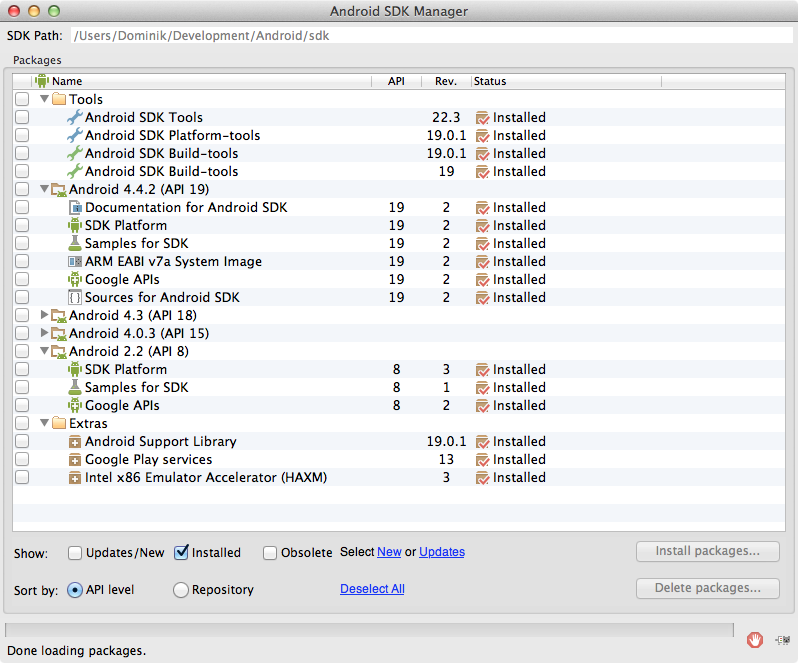
\includegraphics[width=0.85\textwidth]{./images/install/android-sdk-manager.png}
		\caption{SDK Manager: Pakete, die installiert werden müssen.}
		\label{fg:android-sdk-manager}
	\end{figure}
	\item Optional: Falls kein Testgerät vorliegt, welches den Anforderungen entspricht, kann ein „Android Virtual Device“ (AVD)\footnote{http://developer.android.com/tools/devices/index.html} eingerichtet werden. In unseren Tests hat sich ein AVD auf Basis des Nexus One (Abb. \ref{fg:android-adv}) als hilfreich erwiesen. Wichtig ist, dass bei \textit{Target} ein Wert mit \textit{Google APIs} als Präfix ausgewählt wird.
	\begin{figure}[H]
		\centering
		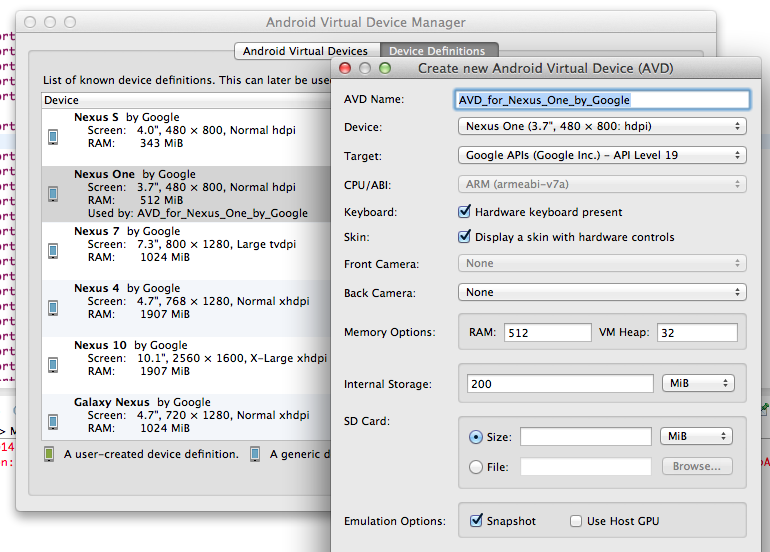
\includegraphics[width=0.85\textwidth]{./images/install/android-avd.png}
		\caption{AVD auf Basis des Nexus One}
		\label{fg:android-adv}
	\end{figure}
\end{enumerate}


\newpage

	%Die Zähler für Tabellen und Abbildungen werden zurückgesetzt, damit
	%in jedem Kapitel die Nummerierung neu beginnt
	\setcounter{table}{1}
	\setcounter{figure}{1}
	%Einbinden des zweiten Kapitels

	%Fazit
	%!TEX root = ../dokumentation.tex

\chapter{Projektreflektion}
Zum Zeitpunkt der Konzeptabgabe stand ein Projektplan mit groben Vorstellungen zum weiteren Projektverlauf.\footnote{Konzeptseite 43} Neben den organisatorischen Meilensteinen zu Abgaben der Artefakte, wurden 2 projektspezifische Meilensteine definiert. Der erste Meilenstein sollte am 25. November erreicht werden und die Bearbeitung des MCI Vorgehens und die Bearbeitung der Proof-of-Concepts beinhalten. 
Anschließend war geplant die Implementation der reinen Funktionalitäten durchzuführen und bis zum 2. Meilenstein am 20. Dezember damit fertig zu werden. Die anschließende Zeit sollte der Gestaltung des Interface gewidmet werden, was wiederrum Gestaltungslösungen der MCI beinhaltet hätte. \\
Bereits nach kurzer Zeit innerhalb der Dokumentationsphase wurde bewusst, dass speziell die Planung der MCI Beschäftigung viel zu knapp bemessen war und sich über den gesamten Projektzeitraum erstrecken sollte. Aufgrund des iterativen Charakters, sollte die Phase bis zum ersten Meilenstein eher als erste Iterationsstufe angesehen werden. Die Überarbeitung des Konzeptes beanspruchte mehr Zeit als anfänglich eingeplant, was zur Folge hatte, dass die eingeplante Zeit für MCI Aspekte weiterhin verkürzt wurde. Als Reaktion darauf, wurde die erste Iterationsphase der MCI Auseinandersetzung bis zum ersten Meilenstein geplant. Zum ersten Test der konzipierten Systemarchitektur, war die Umsetzung der Proof-of-Concepts der erste Schritt, der bis zum ersten Meilenstein ohne Komplikationen durchgeführt werden konnte.\\
Im Laufe des Projektes zeigte sich, dass vorallem zu Beginn einzelne Arbeitsphasen zu grob geplant wurden, was zur Folge hatte das die Auseinandersetzung mit einzelnen Themen mehr Zeit beanspruchte, als ursprünglich gedacht. Bei der organisation des Projektplans wurde auf Excel zurückgegriffen, was zur Folge hatte, dass der Plan bei zunehmender Projektdauer und Verfeinerung der unübersichtlich wurde, letzendlich aber keinen Einfluss auf das Zeitmanagement an sich hat.\\

Rückblickend bedeutete sowohl die MCI Auseinandersetzung als auch die Implementation des Systems mehr Arbeit, als in der gegeben Zeit investiert werden konnte. 
Auf zeitliche Rückschläge wurde an gegeben Stellen reagiert, jedoch hätte eine konkretere Fokusierung auf wesentliche Aspekte die Entwicklungszeit eventuell kontrollierbarer gestaltet.\\ 

Zahlreiche Techniken der MCI wurden durchgeführt, letztendlich reichte es aber zeitlich nicht den finalen Prototypen zu evaluieren und auf diese Art in ein Interface umzusetzen. Während des Projektverlaufs wäre eine gezieltere Wahl der Methoden an gegeben Stellen von Vorteil gewesen, um zusätzlichen Aufwand und Überarbeitung zu vermeiden. Die Auseinandersetzung mit den Benutzern und ihren Aufgaben fand in einem umfangreichen Rahmen statt und sind nach eigenem Ermessen eine gute Grundlage für weitere Iterationsphasen.\\

Zu Beginn der Konzeptphase, wurden eigene Ziele an das Projekt in Form einer Zielhierachie definiert.\footnote{Konzeptkapitel 6}
In Hinblick auf das Alleinstellungsmerkmal wurde dabei das Minimalziel beschrieben, dass auf der Vermittlung zwischen Mieter und Vermieter lag und die Kontaktaufnahme beider Parteien ermöglicht. Da in Anbetracht der Systemdokumentation, wesentliche Aspekten umgesetzt werden konnten, gilt zumindest dieses Ziel als weitestgehend erfüllt.

	%Fazit
	%!TEX root = ../dokumentation.tex

\addcontentsline{toc}{chapter}{Literaturverzeichnis}
\chapter*{Literatur- und Quellenverzeichnis}
Literaturquellen 
\begin{itemize}
\item
Prof. Dr. Gerhard Hartmann: Draft zum kleinen Handbuch der Mensch-Computer Interaktion, März 2013
\item
L. Constantine \& L. Lockwood: Software for use, 2003
\item 
David Benyon: Designing Interactive Systems, A comprehensive guide to HCI and interaction Design (2nd Edition) 
\item
ISO 9241-210: Human-centred design for interactive systems nach Draft von Prof. Dr. Hartmann,
\\http://www.iso.org/iso/catalogue\_detail.htm?csnumber=52075

\end{itemize}

Internetquellen 
\begin{itemize}
\item
Grunddlegenede Publikationen zum Usage centered Design \\http://www.foruse.com/questions/index.htm\#13 letztes Sichtdatum 09.01.2014

\item
Larry L Constanine Rapid Abstract Prototyping, PDF über \\ http://www.foruse.com/articles/abstractprototypes.htm

\end{itemize}

\newpage

 
%Zeilenabstand 1 fach für die Verzeichnisse
\singlespacing
%Einbindne der Verzeichnisse
%!TEX root = ../Dokumentation.tex

  %Erzeugt ein Abbildungsverzeichnis
	\listoffigures
	%Fügt die Zeile "`Abbildungsverzeichnis"' als Chapter ins Inhaltsverzeichnis ein
	\addcontentsline{toc}{chapter}{Abbildungsverzeichnis}

	%Erzeugt ein Tabellenverzeichnis
	\listoftables
	%Fügt die Zeile "`Tabellenverzeichnis"' als Chapter ins Inhaltsverzeichnis ein
	\addcontentsline{toc}{chapter}{Tabellenverzeichnis}

	%Erzeugt ein Codeverzeichnis
	\lstlistoflistings
	%Fügt die Zeile "`Codeverzeichnis"' als Chapter ins Inhaltsverzeichnis ein
	\addcontentsline{toc}{chapter}{Codeverzeichnis}

	%Erzeugt ein Glossar
%	\printnomenclature
	%Fügt die Zeile "`Glossar"' als Chapter ins Inhaltsverzeichnis ein
%	\addcontentsline{toc}{chapter}{Glossar}

	%Ändert den Stil des Literaturverzeichnisses
	\bibliographystyle{geralpha}
	%Erzeugt das Literaturverzeichnis anhand der Datei "`literatur.bib"'
%	\bibliography{doc/literatur}
	%Fügt die Zeile "`Literaturverzeichnis"' als Chapter ins Inhaltsverzeichnis ein
%	\addcontentsline{toc}{chapter}{Literaturverzeichnis}


%Zeilenabstand 1,5 fach für den Eid
\onehalfspacing
%Einbinden des Eides
%%!TEX root = ../konzept.tex

\chapter*{Eidesstattliche Erklärung}
\addcontentsline{toc}{chapter}{Eidesstattliche Erklärung}
Ich versichere, die von mir vorgelegte Arbeit selbständig verfasst zu haben.\\ \\
Alle Stellen, die wörtlich oder sinngemäß aus veröffentlichten oder nicht veröffentlichten Arbeiten anderer entnommen sind, habe ich als entnommen kenntlich gemacht. Sämtliche Quellen und Hilfsmittel, die ich für die Arbeit benutzt habe, sind angegeben.\\ \\
Die Arbeit hat mit gleichem Inhalt bzw. in wesentlichen Teilen noch keiner anderen Prüfungsgbehörde vorgelegen.
\vspace{1.5cm}
\\
Gummersbach, 28. Oktober 2013
\vspace{3cm}
\\
Dennis Meyer \\
Dominik Schilling


%Konzept als Anhang einbinden
%!TEX root = ../dokumentation.tex

\chapter{Abstract Prototype 1}

%Seite 1
\begin{figure}[H]
\centering
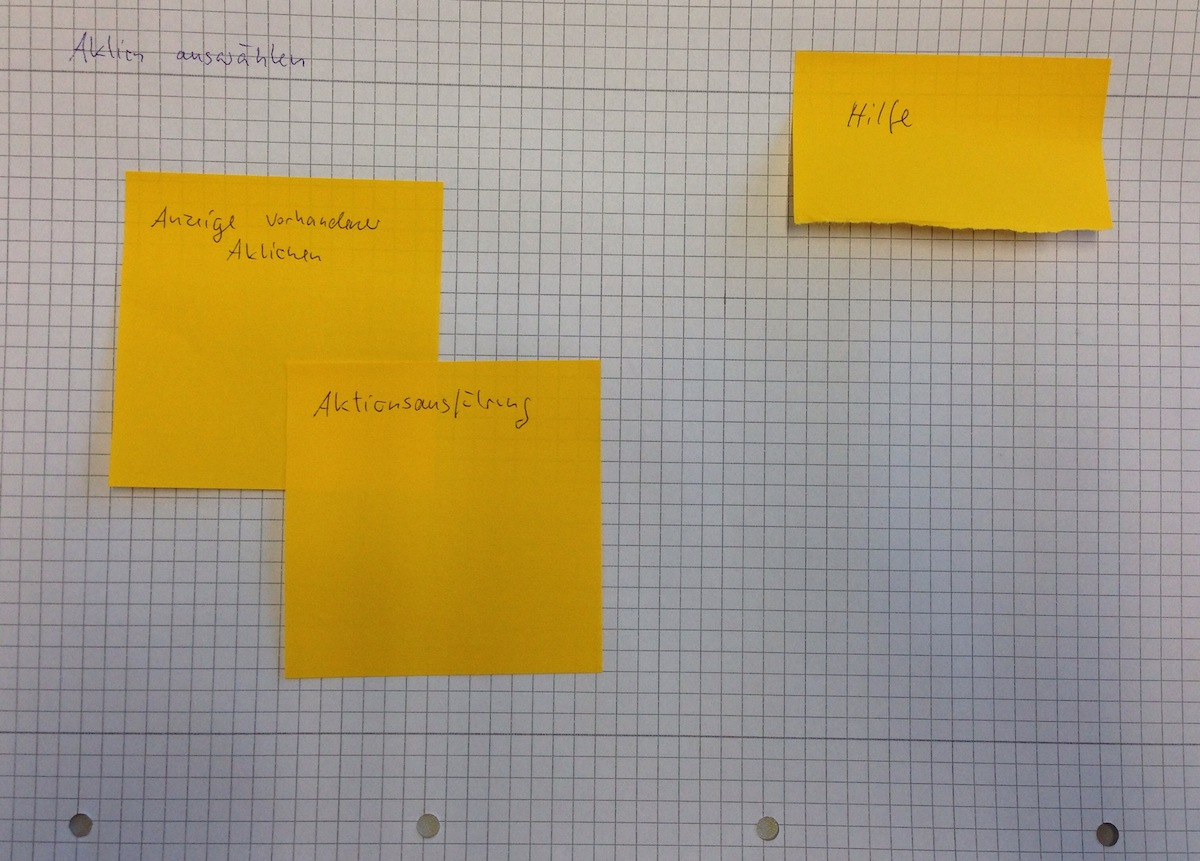
\includegraphics[width=0.85\textwidth]{./images/abstract/version1/aktionAuswaehlen.JPG}
\caption{Interaction Context AP1: aktionAuswählen}
\label{interfaceContents20}
\end{figure}

\begin{figure}[H]
\centering
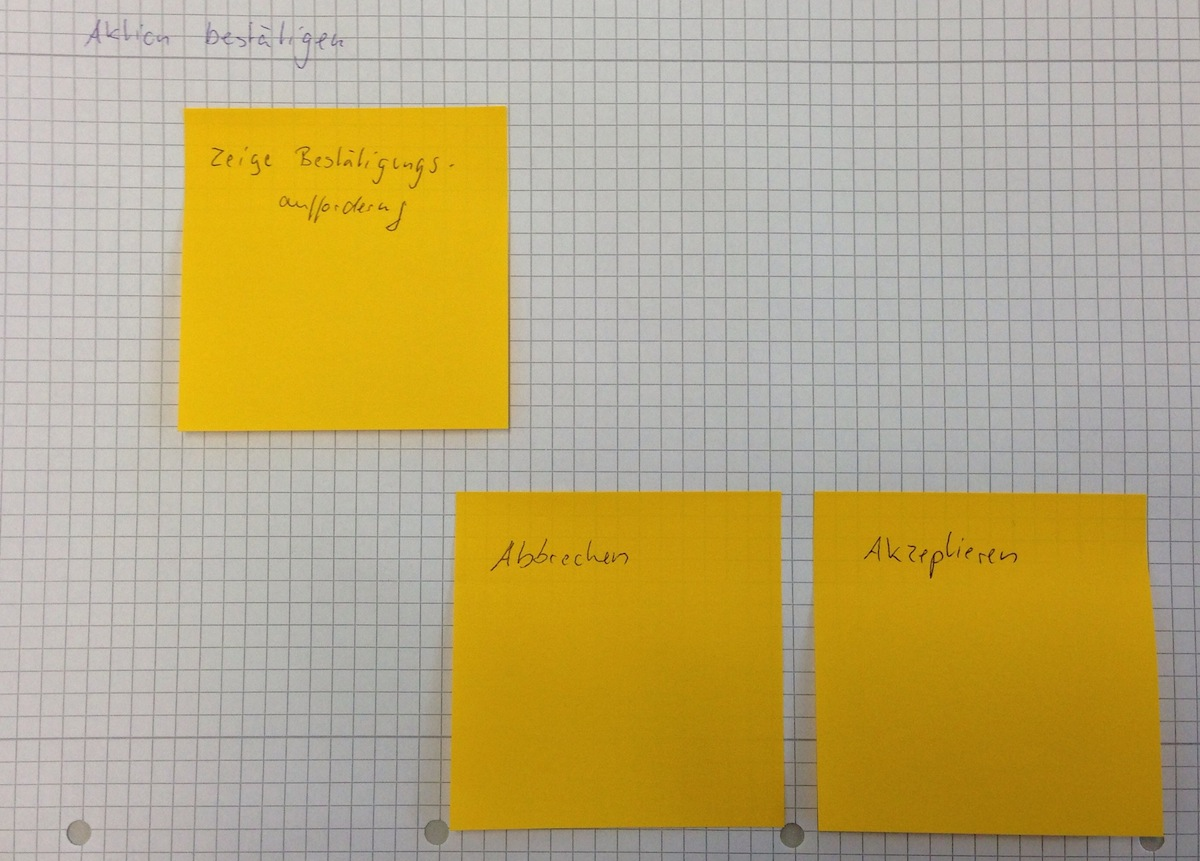
\includegraphics[width=0.85\textwidth]{./images/abstract/version1/aktionBestaetigen.JPG}
\caption{Interaction Context AP1: aktionBestätigen}
\label{interfaceContents21}
\end{figure}


%Seite 2
\begin{figure}[H]
\centering
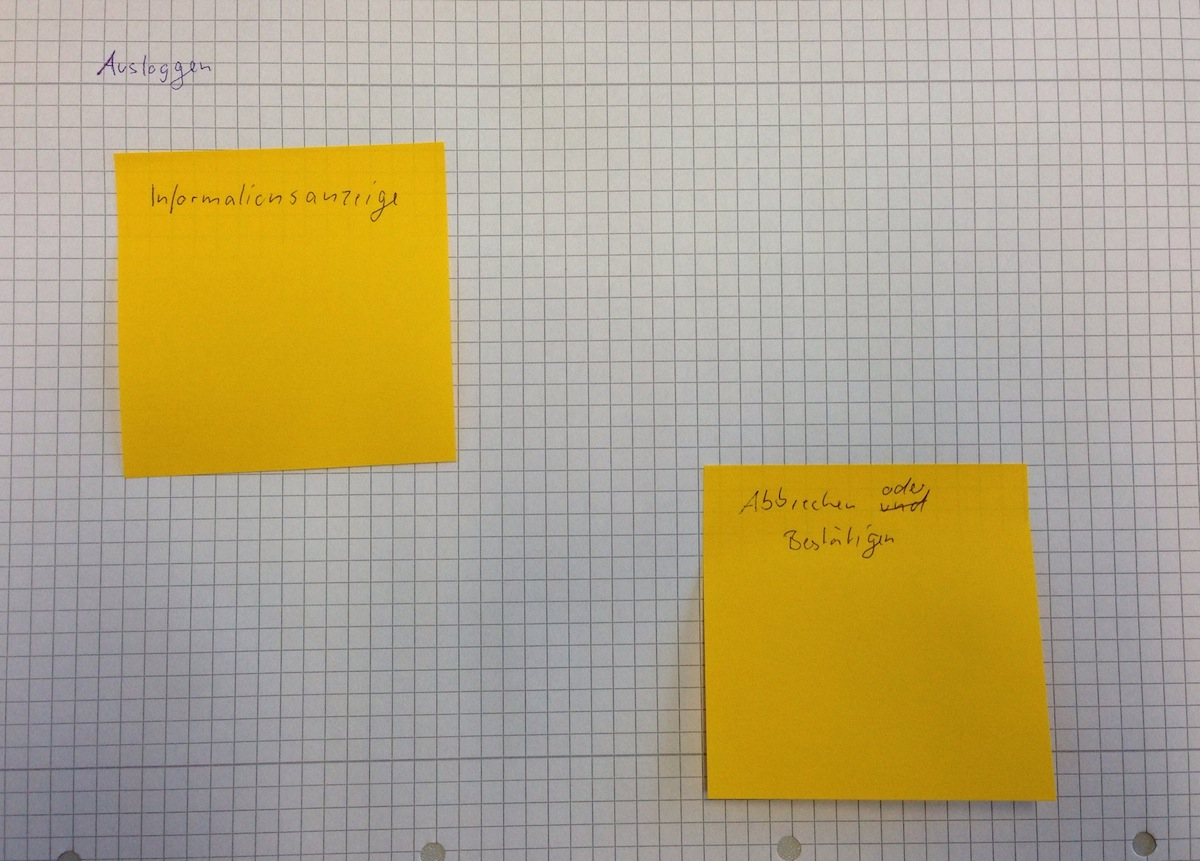
\includegraphics[width=0.85\textwidth]{./images/abstract/version1/ausloggen.JPG}
\caption{Interaction Context AP1: ausloggen}
\label{interfaceContents22}
\end{figure}

\begin{figure}[H]
\centering
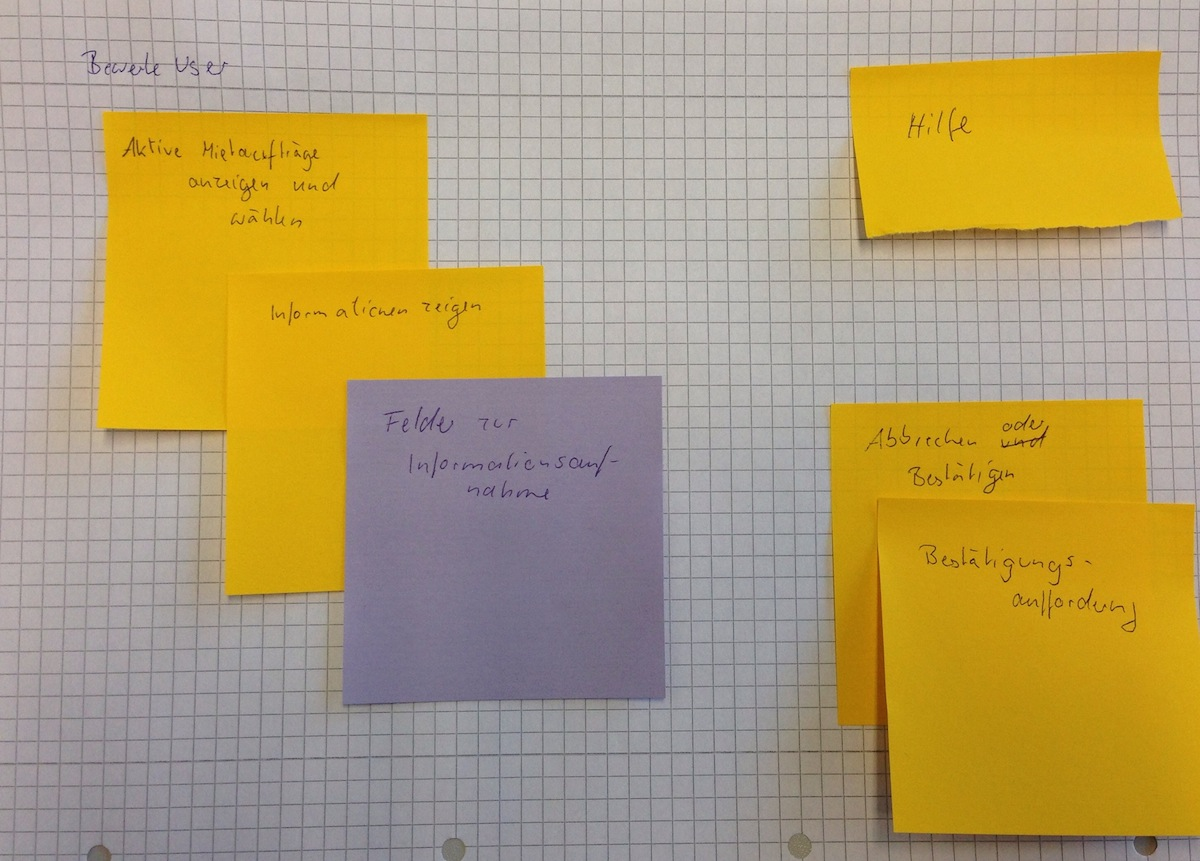
\includegraphics[width=0.85\textwidth]{./images/abstract/version1/bewerteUser.JPG}
\caption{Interaction Context AP1: bewerteUser}
\label{interfaceContents23}
\end{figure}


%Seite 3
\begin{figure}[H]
\centering
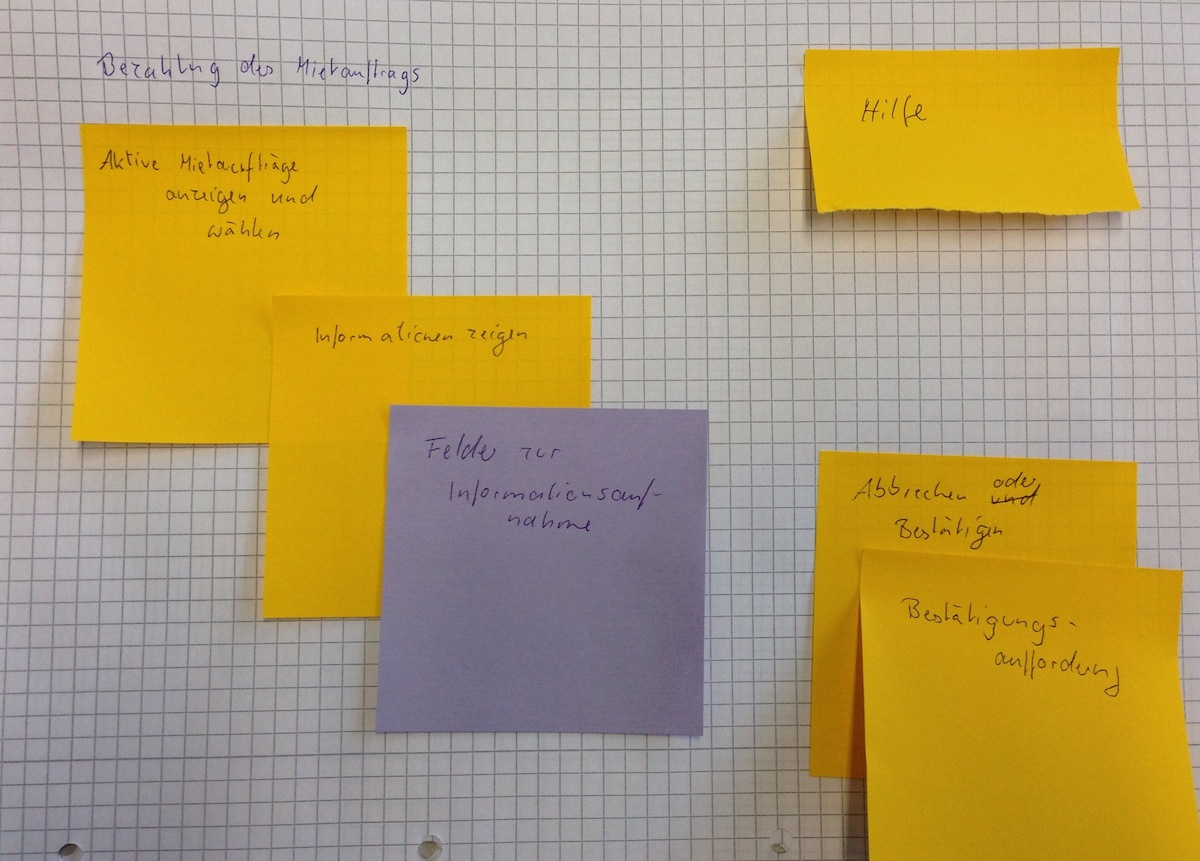
\includegraphics[width=0.85\textwidth]{./images/abstract/version1/bezahlungDesMietauftrags.JPG}
\caption{Interaction Context AP1: bezahlungDesMietauftrags}
\label{interfaceContents24}
\end{figure}

\begin{figure}[H]
\centering
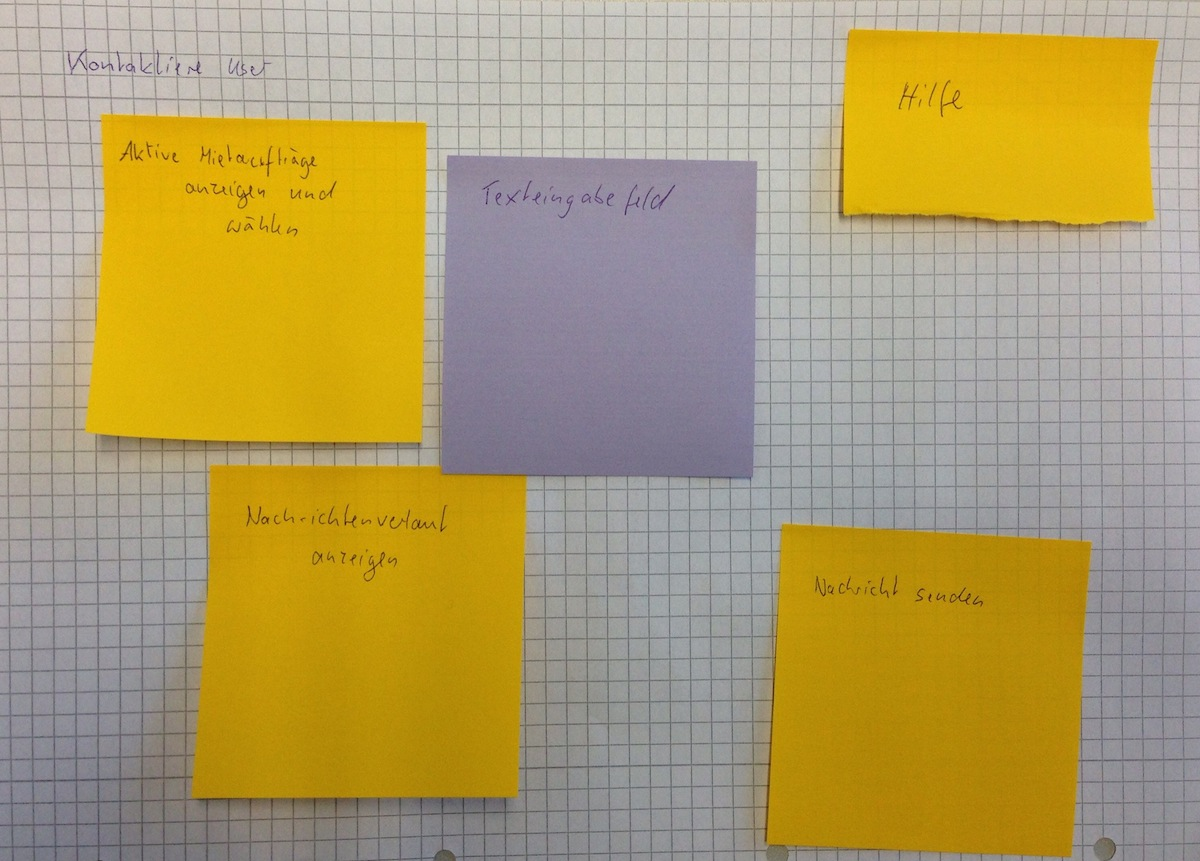
\includegraphics[width=0.85\textwidth]{./images/abstract/version1/kontaktiereUser.JPG}
\caption{Interaction Context AP1: kontaktiereUser}
\label{interfaceContents25}
\end{figure}


%Seite 4
\begin{figure}[H]
\centering
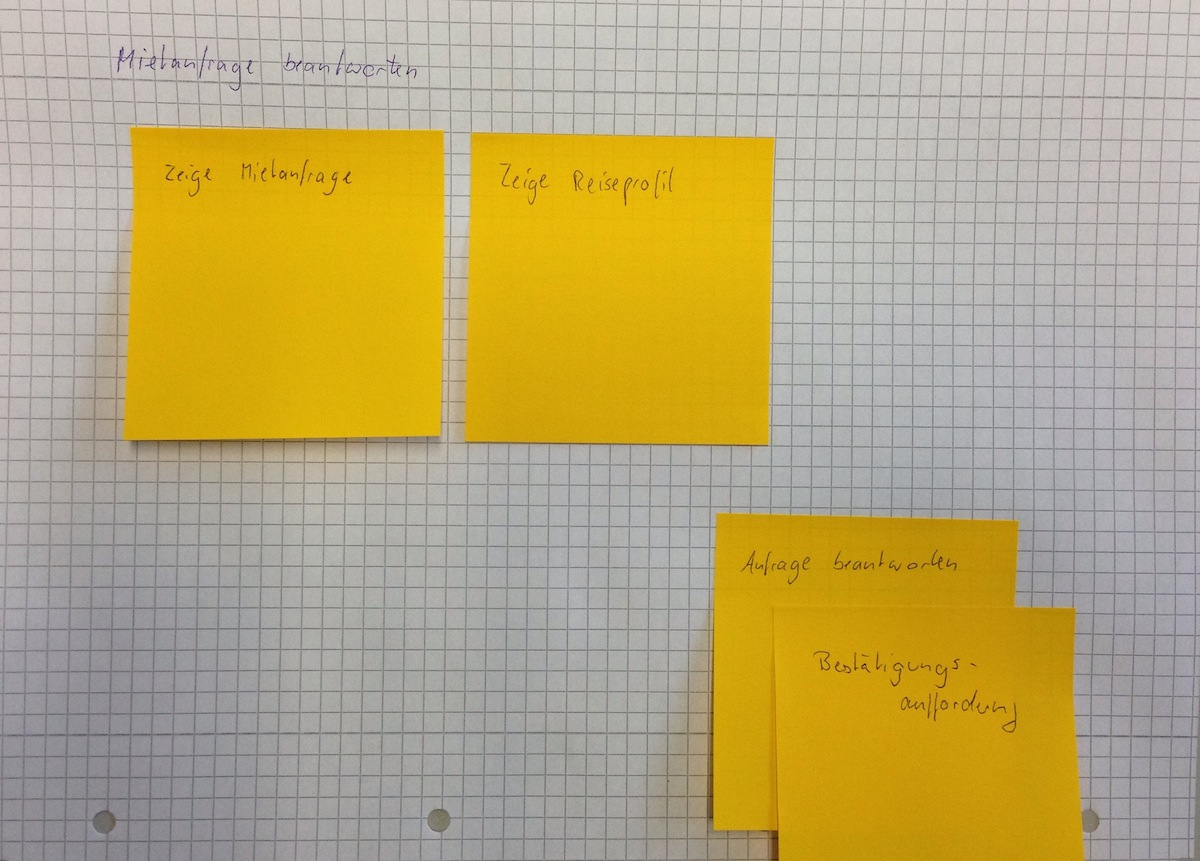
\includegraphics[width=0.85\textwidth]{./images/abstract/version1/mietanfrageBeantworten.JPG}
\caption{Interaction Context AP1: mietanfrageBeantworten}
\label{interfaceContents26}
\end{figure}

\begin{figure}[H]
\centering
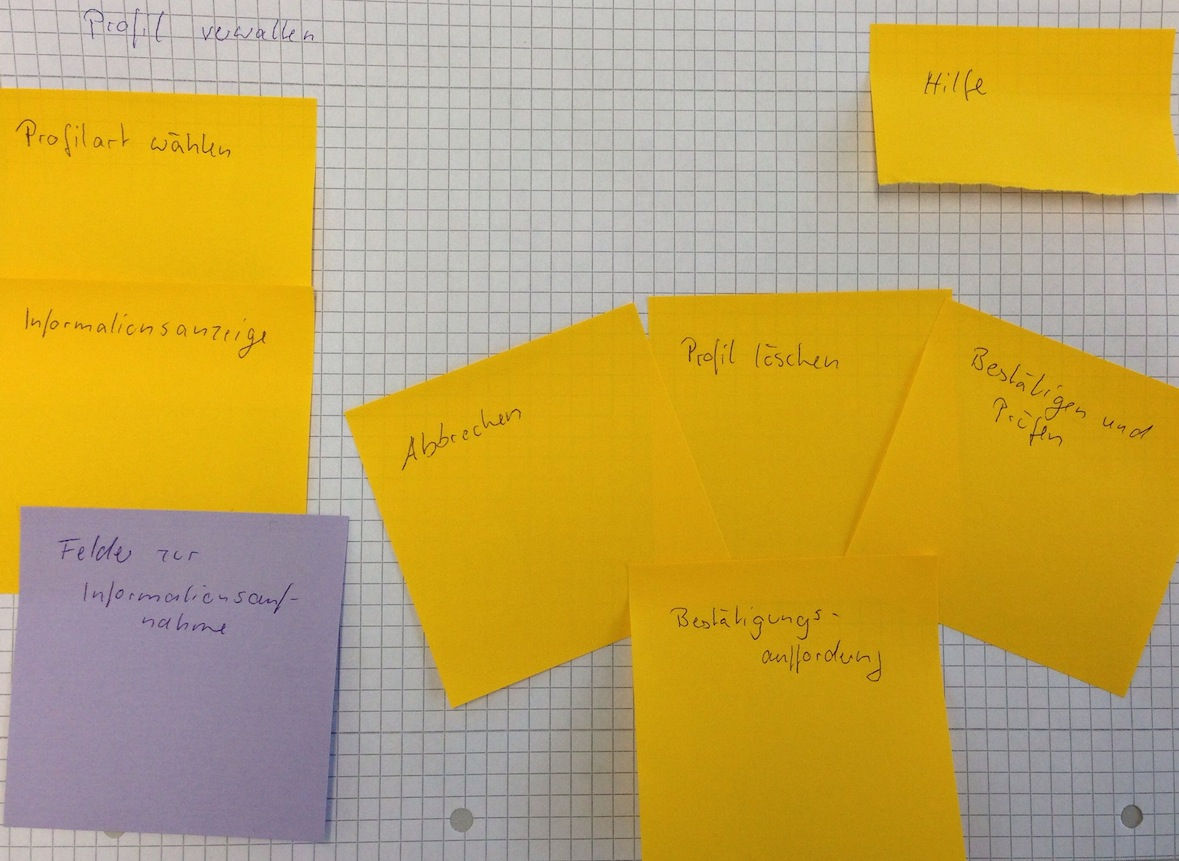
\includegraphics[width=0.85\textwidth]{./images/abstract/version1/profilVerwalten.JPG}
\caption{Interaction Context AP1: profilVerwalten}
\label{interfaceContents27}
\end{figure}


%Seite 5
\begin{figure}[H]
\centering
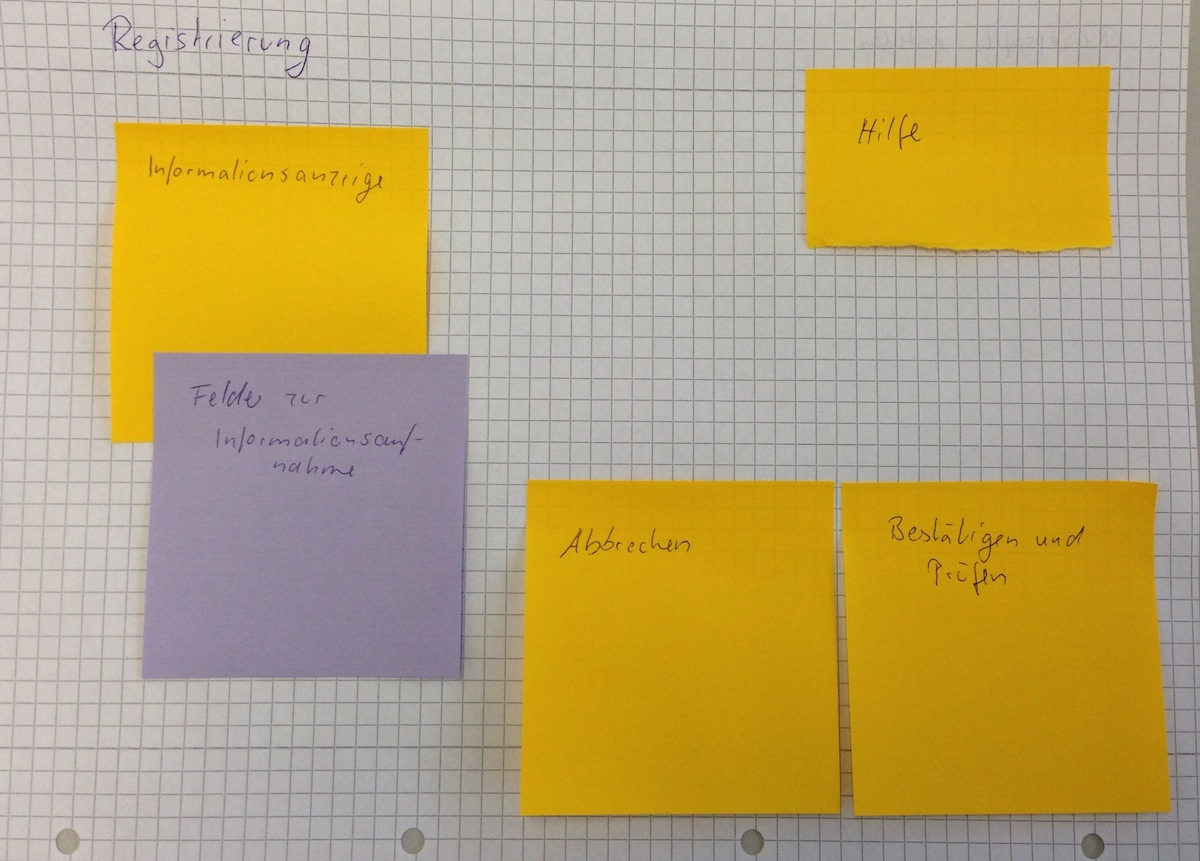
\includegraphics[width=0.85\textwidth]{./images/abstract/version1/registrierung.JPG}
\caption{Interaction Context AP1: registrierung}
\label{interfaceContents28}
\end{figure}

\begin{figure}[H]
\centering
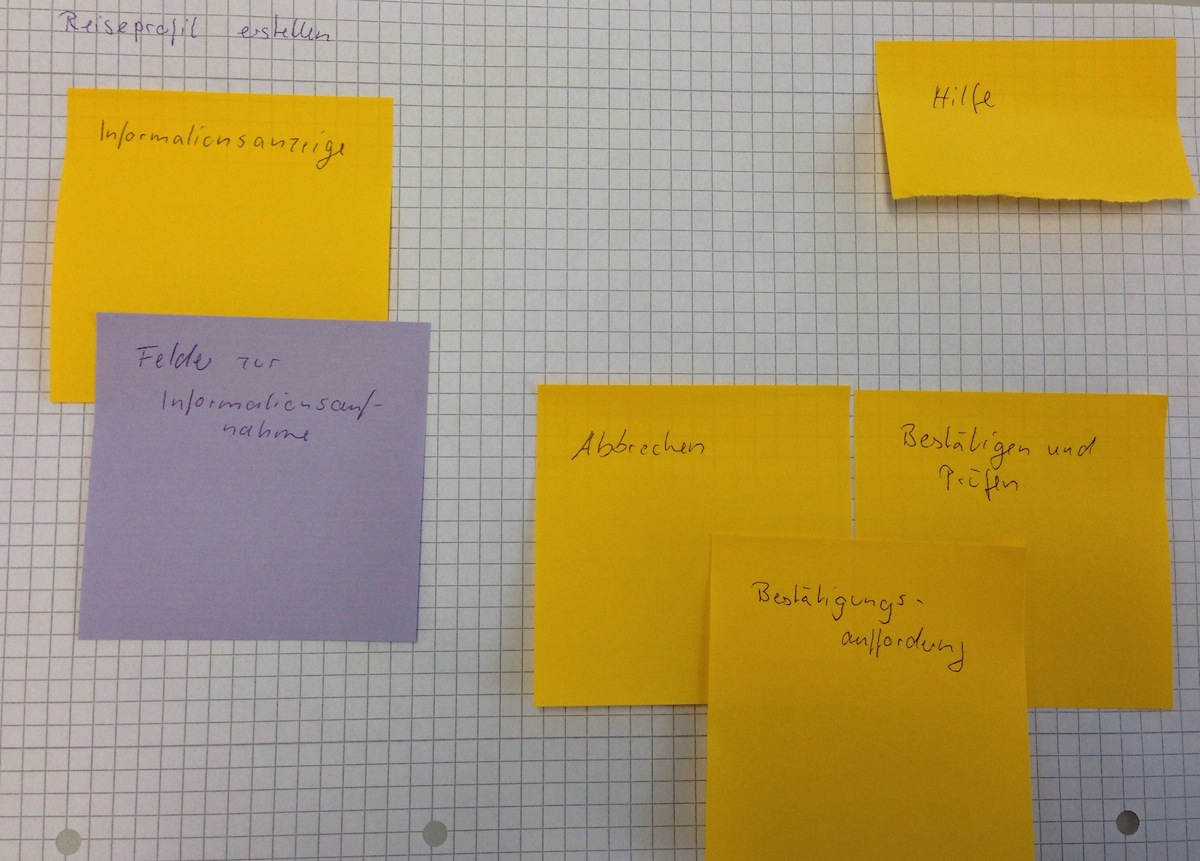
\includegraphics[width=0.85\textwidth]{./images/abstract/version1/reiseprofilErstellen.JPG}
\caption{Interaction Context AP1: reiseprofilErstellen}
\label{interfaceContents29}
\end{figure}

%Seite 6
\begin{figure}[H]
\centering
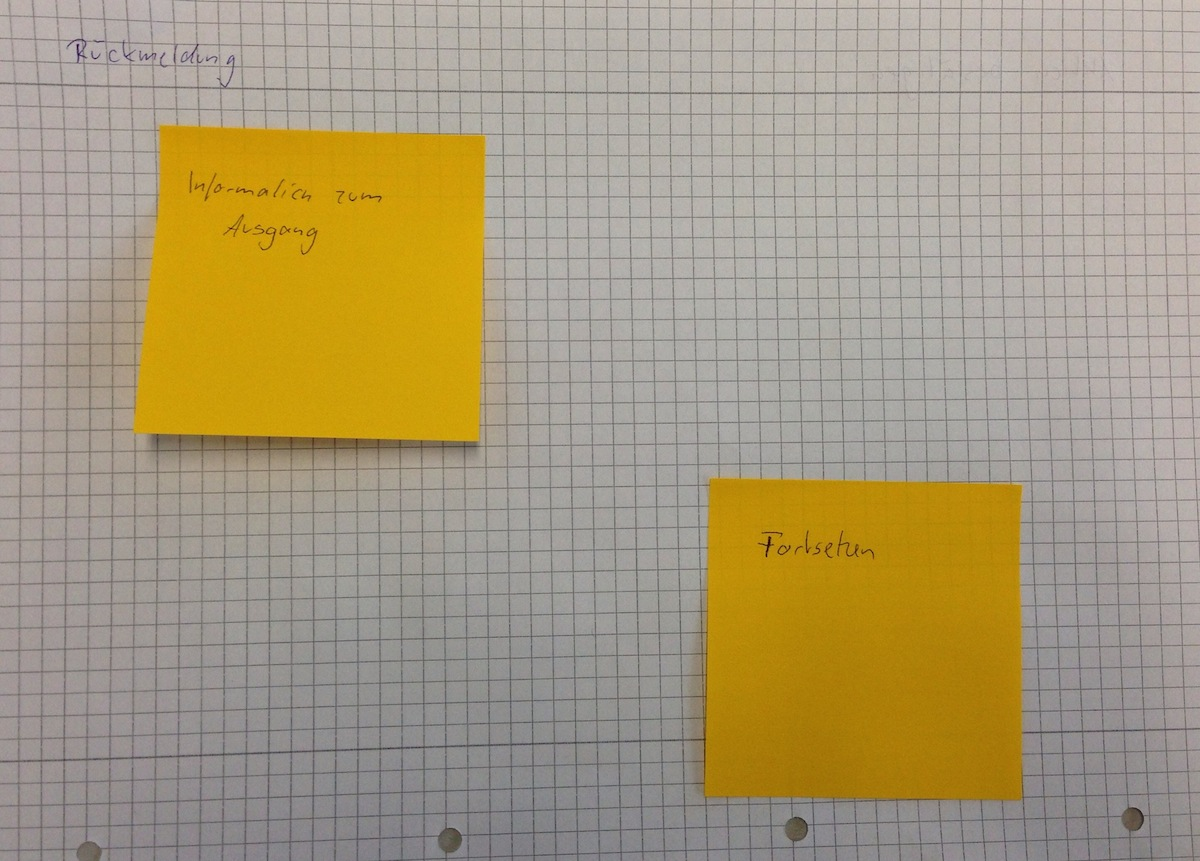
\includegraphics[width=0.85\textwidth]{./images/abstract/version1/rueckmeldung.JPG}
\caption{Interaction Context AP1: rueckmeldung}
\label{interfaceContents30}
\end{figure}

\begin{figure}[H]
\centering
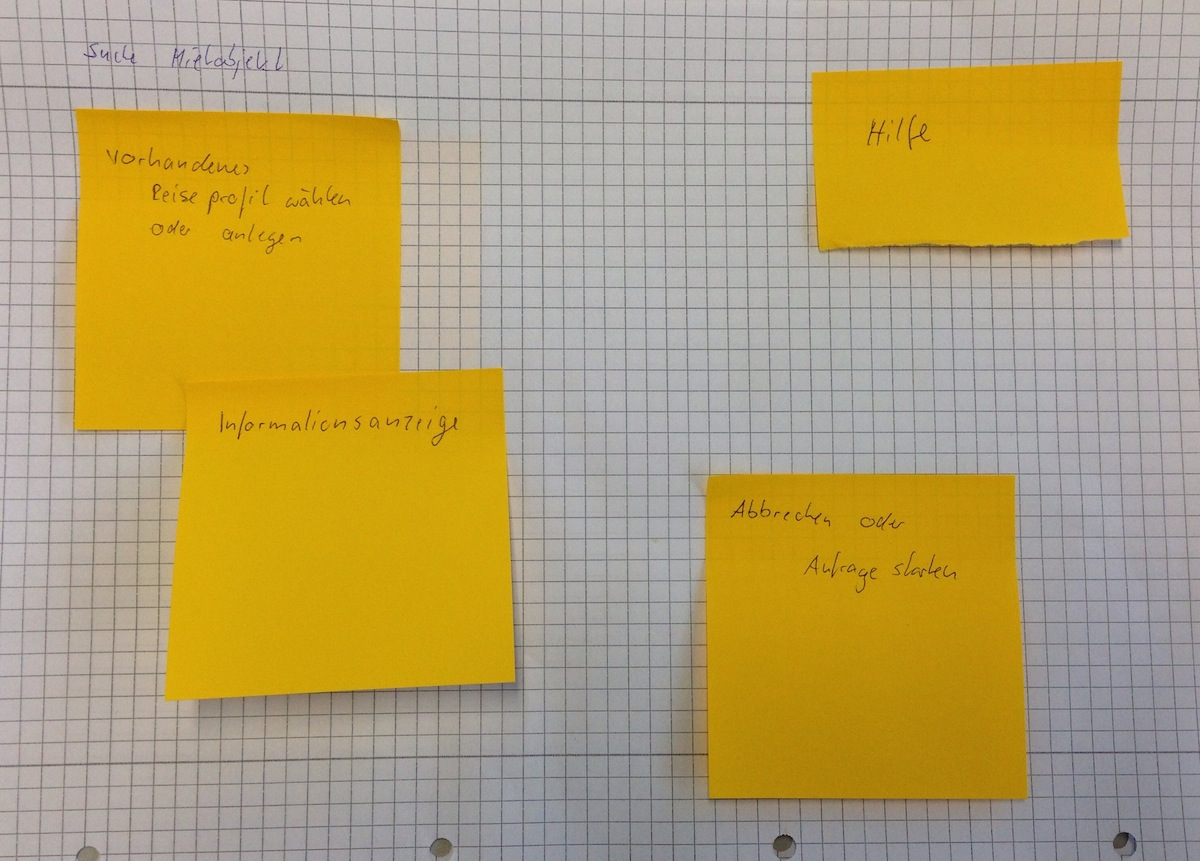
\includegraphics[width=0.85\textwidth]{./images/abstract/version1/sucheMietobjekt.JPG}
\caption{Interaction Context AP1: sucheMietobjekt}
\label{interfaceContents31}
\end{figure}


\chapter{Abstract Prototype 2}

%Seite 1
\begin{figure}[H]
\centering
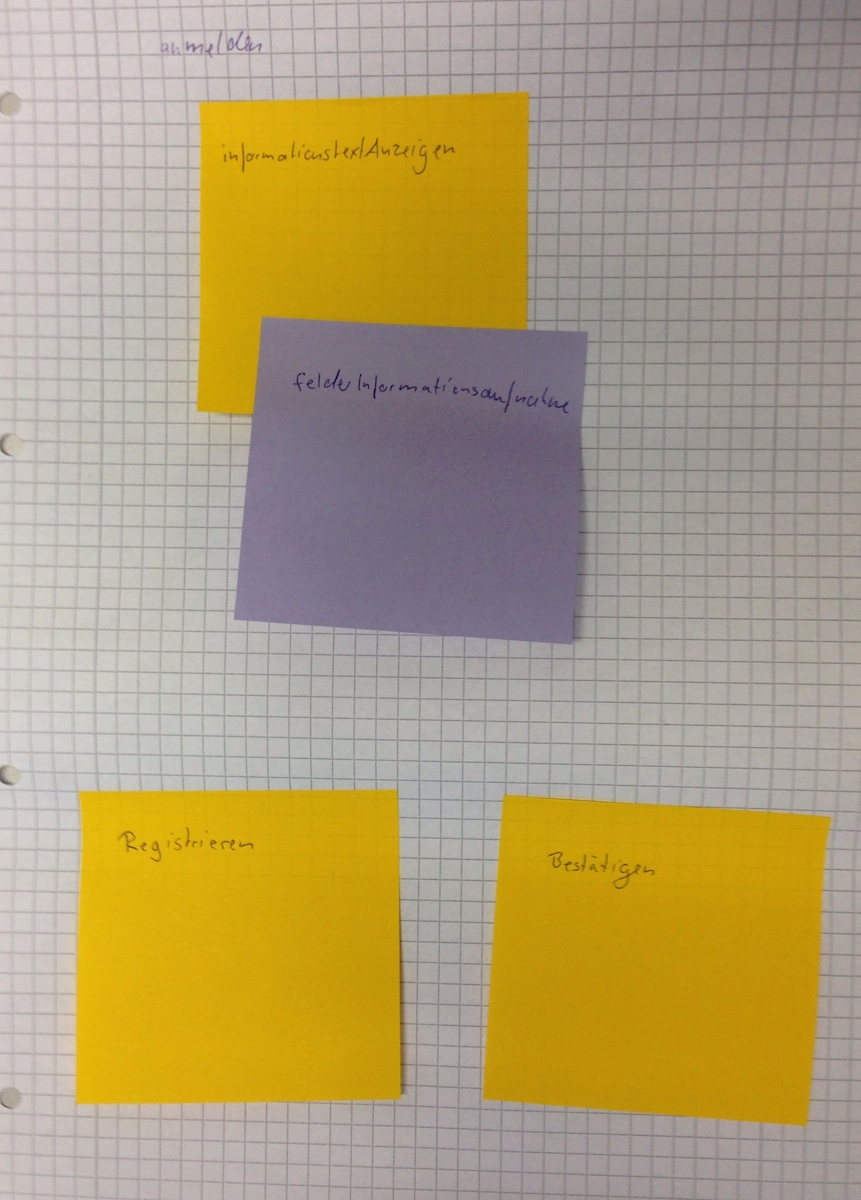
\includegraphics[angle=90, width=0.85\textwidth] {./images/abstract/version2/anmelden.JPG}
\caption{Interaction Context AP2: anmelden}
\label{interfaceContents40}
\end{figure}

\begin{figure}[H]
\centering
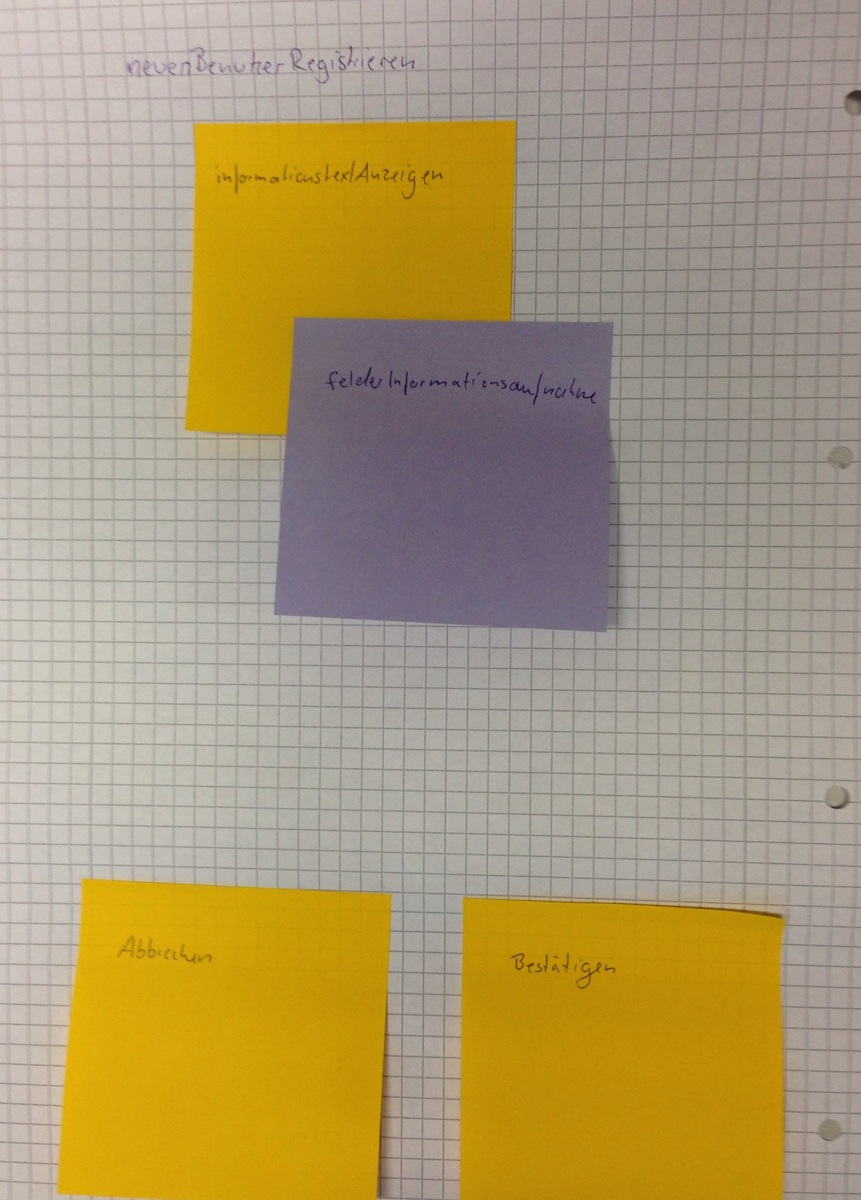
\includegraphics[angle=90, width=0.85\textwidth]  {./images/abstract/version2/neuenBenutzerRegistrieren.JPG}
\caption{Interaction Context AP2: neuenBenutzerRegistrieren}
\label{interfaceContents41}
\end{figure}

%Seite 2
\begin{figure}[H]
\centering
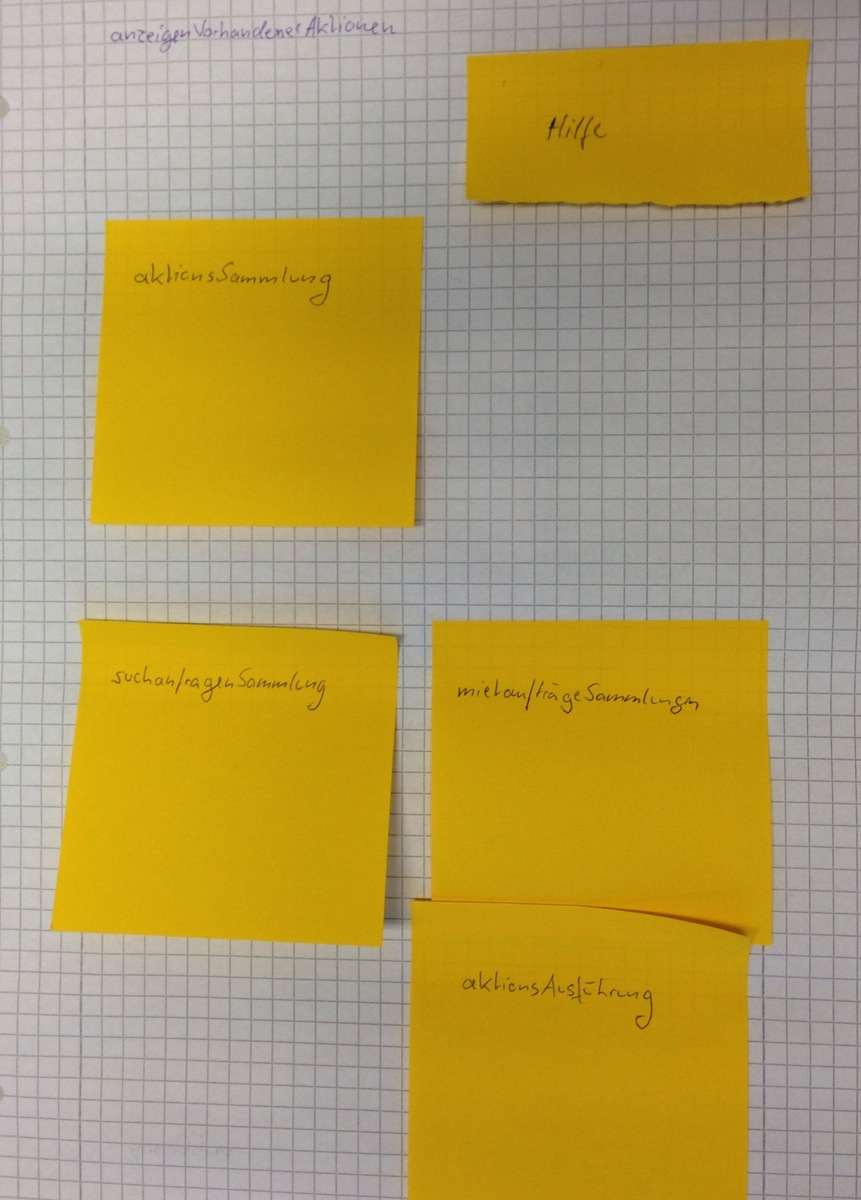
\includegraphics[angle=90, width=0.85\textwidth] {./images/abstract/version2/anzeigenVorhandenerAktionen.JPG}
\caption{Interaction Context AP2: anzeigenVorhandenerAktionen}
\label{interfaceContents42}
\end{figure}

\begin{figure}[H]
\centering
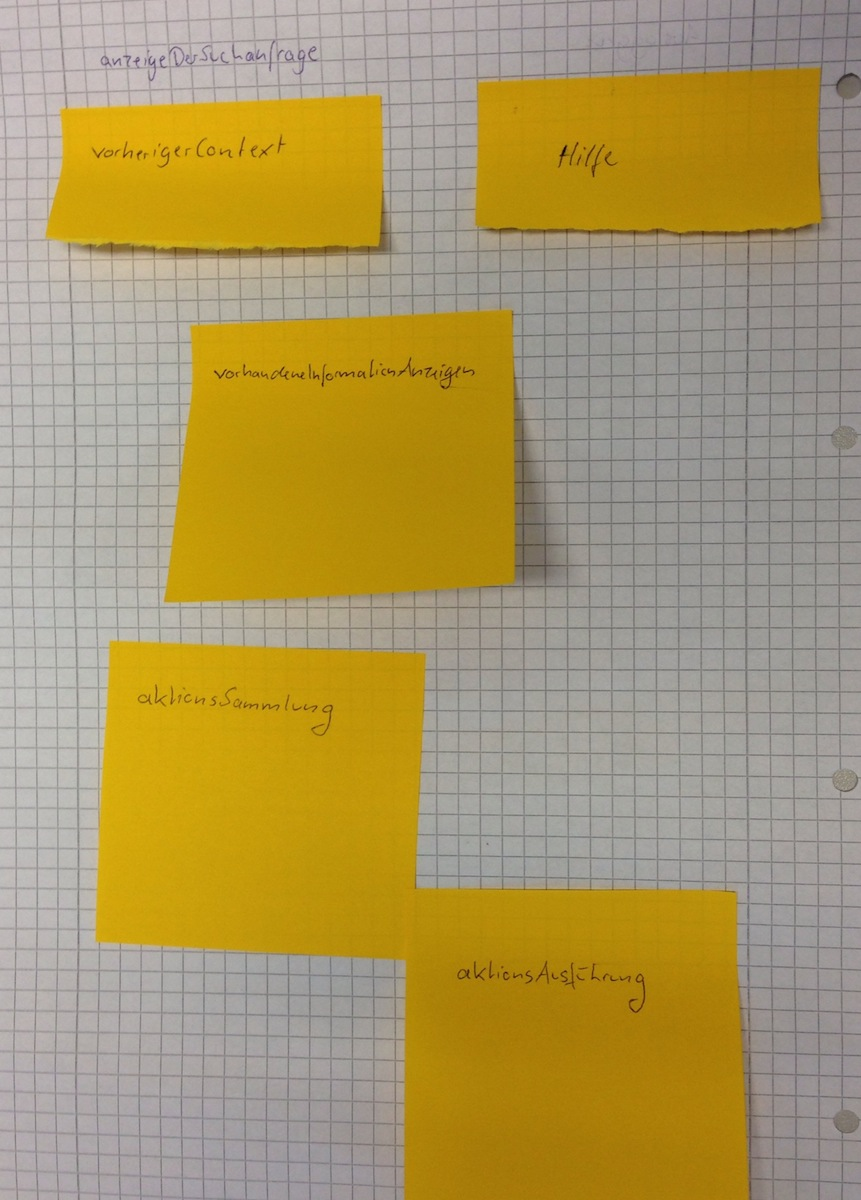
\includegraphics[angle=90, width=0.85\textwidth]  {./images/abstract/version2/anzeigeDerSuchanfrage.JPG}
\caption{Interaction Context AP2: anzeigeDerSuchanfrage}
\label{interfaceContents43}
\end{figure}


%Seite 3
\begin{figure}[H]
\centering
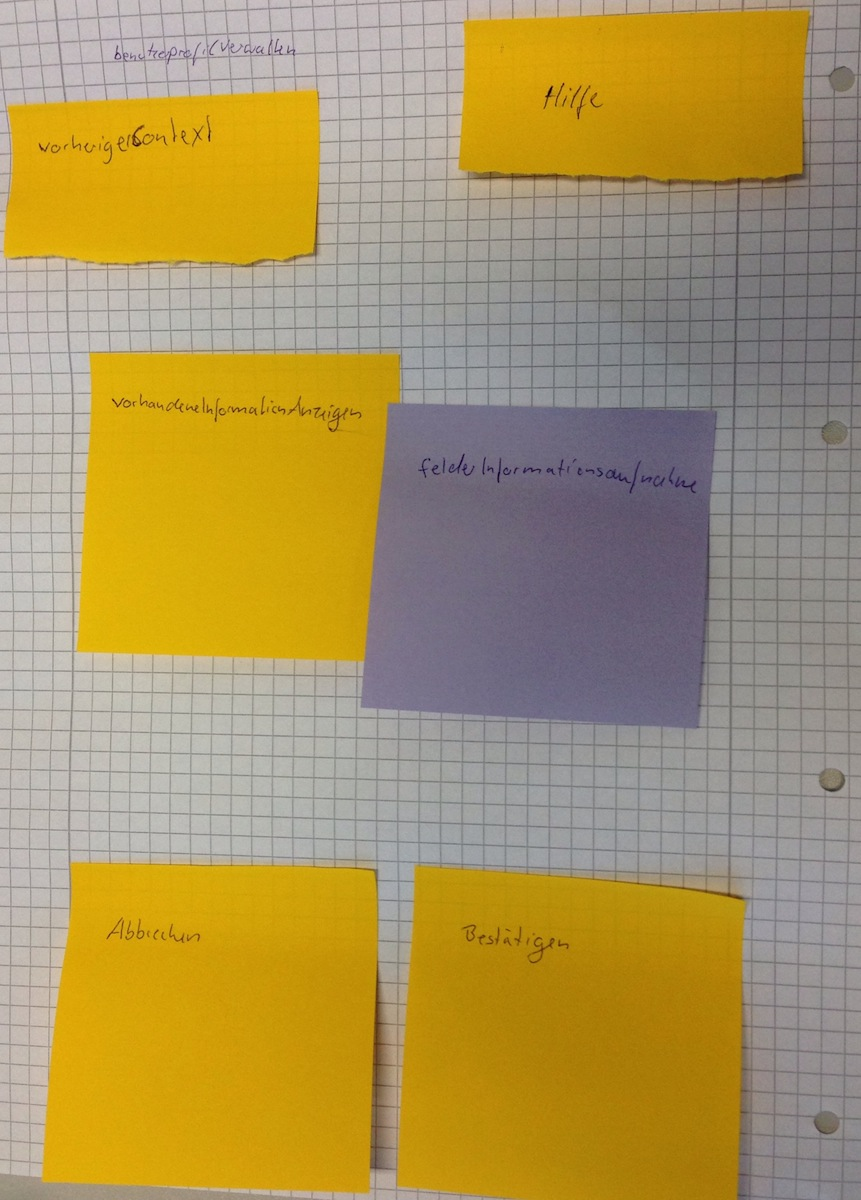
\includegraphics[angle=90, width=0.85\textwidth] {./images/abstract/version2/benutzerprofilVerwalten.JPG}
\caption{Interaction Context AP2: benutzerprofilVerwalten}
\label{interfaceContents44}
\end{figure}

\begin{figure}[H]
\centering
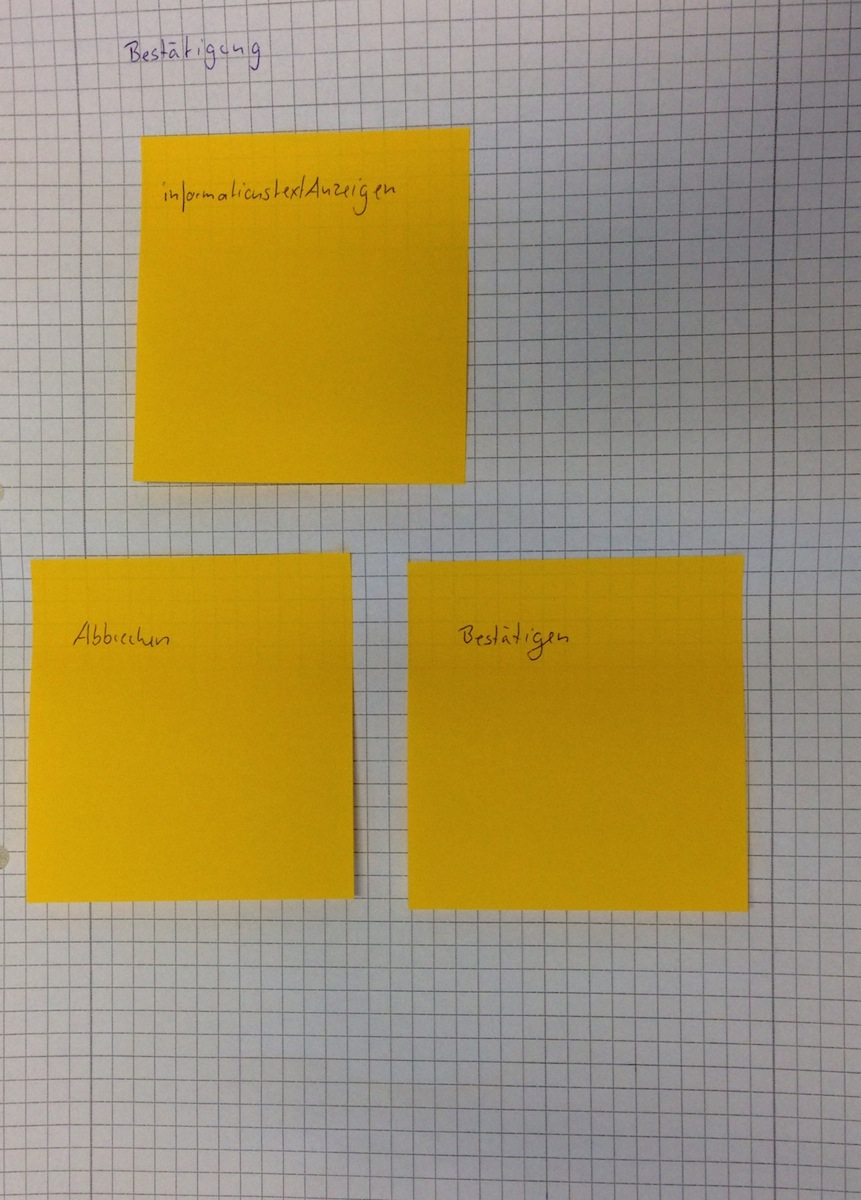
\includegraphics[angle=90, width=0.85\textwidth]  {./images/abstract/version2/bestaetigung.JPG}
\caption{Interaction Context AP2: bestätigung}
\label{interfaceContents45}
\end{figure}


%Seite 4
\begin{figure}[H]
\centering
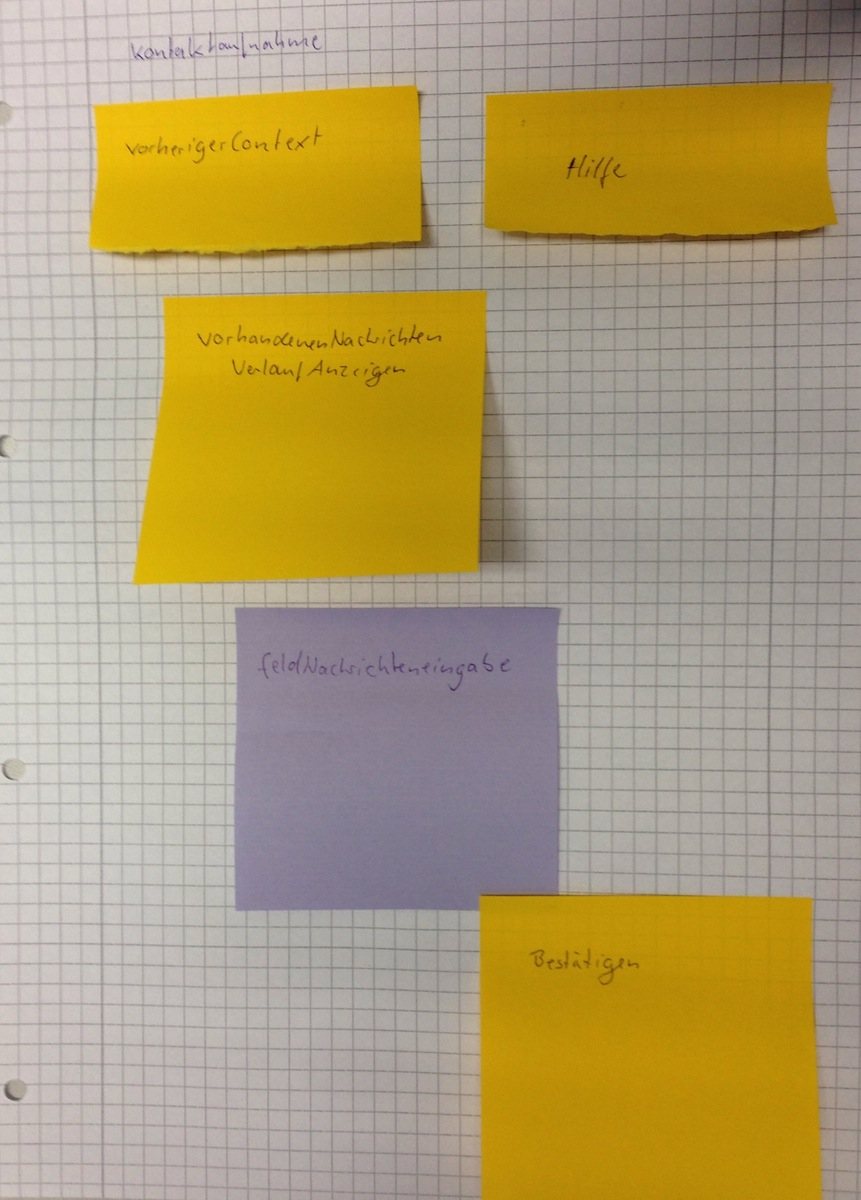
\includegraphics[angle=90, width=0.85\textwidth] {./images/abstract/version2/kontaktaufnahme.JPG}
\caption{Interaction Context AP2: kontaktaufnahme}
\label{interfaceContents46}
\end{figure}

\begin{figure}[H]
\centering
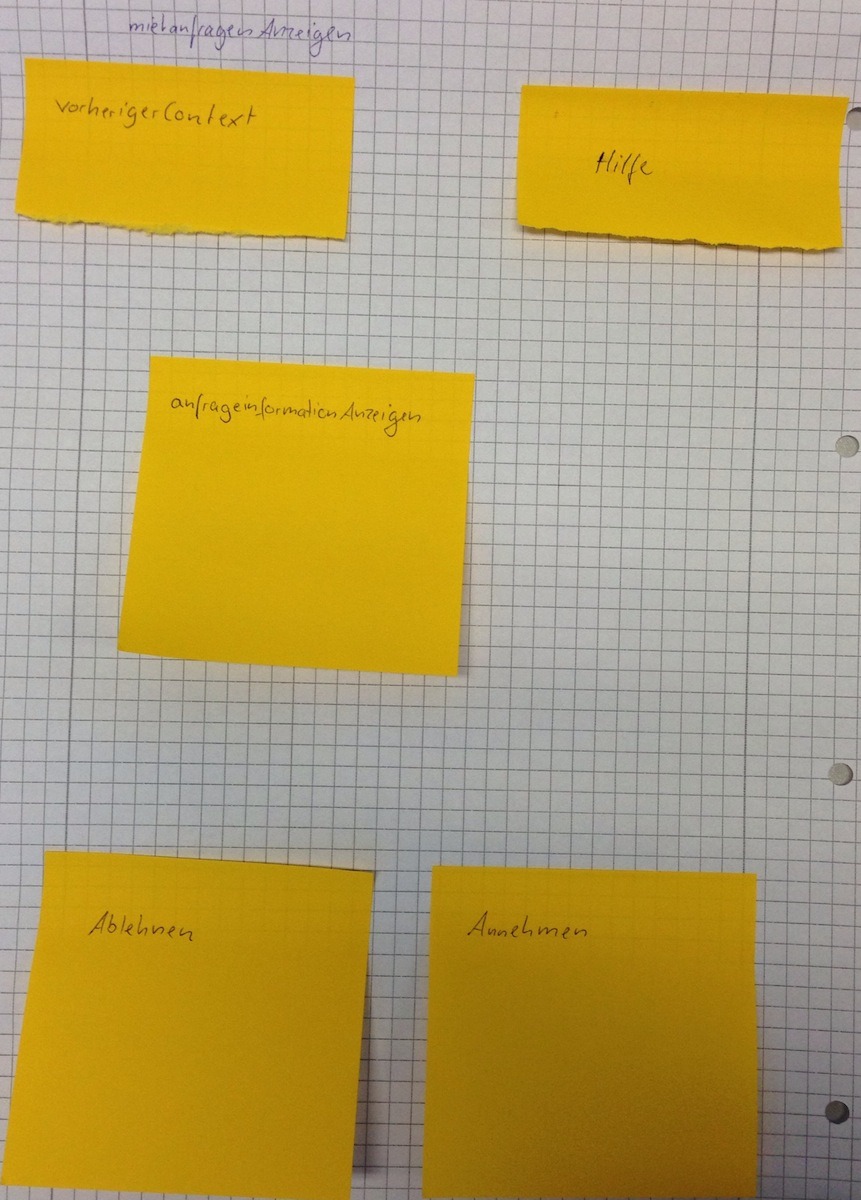
\includegraphics[angle=90, width=0.85\textwidth]  {./images/abstract/version2/mietanfragenAnzeigen.JPG}
\caption{Interaction Context AP2: mietanfragenAnzeigen}
\label{interfaceContents47}
\end{figure}


%Seite 5
\begin{figure}[H]
\centering
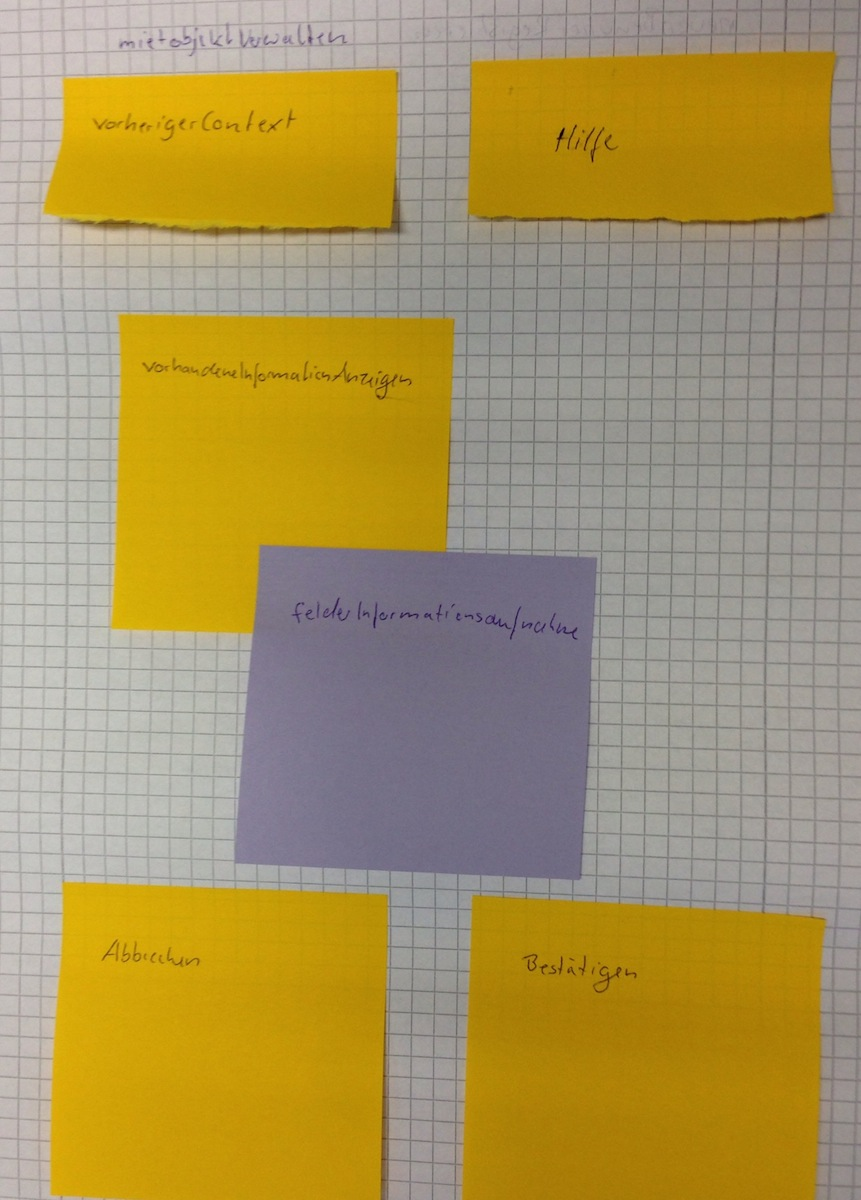
\includegraphics[angle=90, width=0.85\textwidth] {./images/abstract/version2/mietobjekteVerwalten.JPG}
\caption{Interaction Context AP2: mietobjekteVerwalten}
\label{interfaceContents48}
\end{figure}

\begin{figure}[H]
\centering
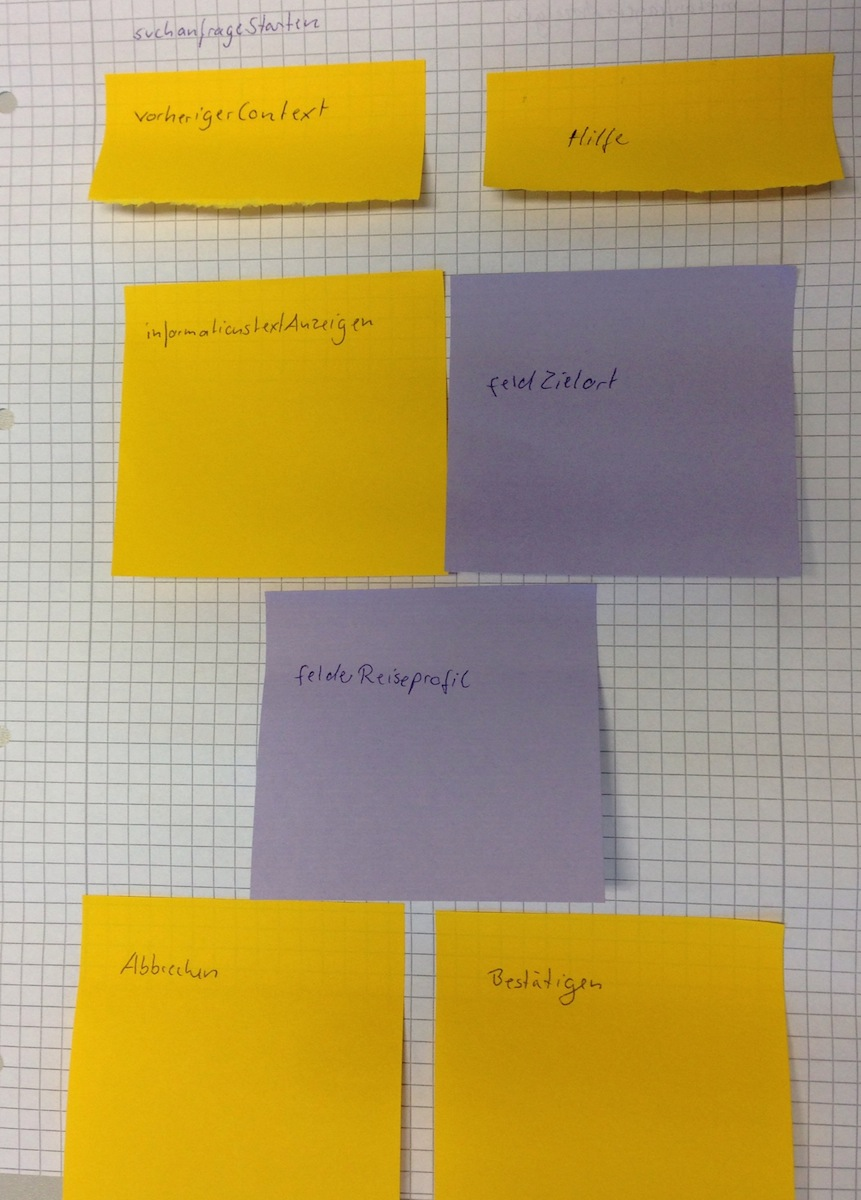
\includegraphics[angle=90, width=0.85\textwidth]  {./images/abstract/version2/suchanfragenStarten.JPG}
\caption{Interaction Context AP2: suchanfrageStarten}
\label{interfaceContents49}
\end{figure}


%Seite 6
\begin{figure}[H]
\centering
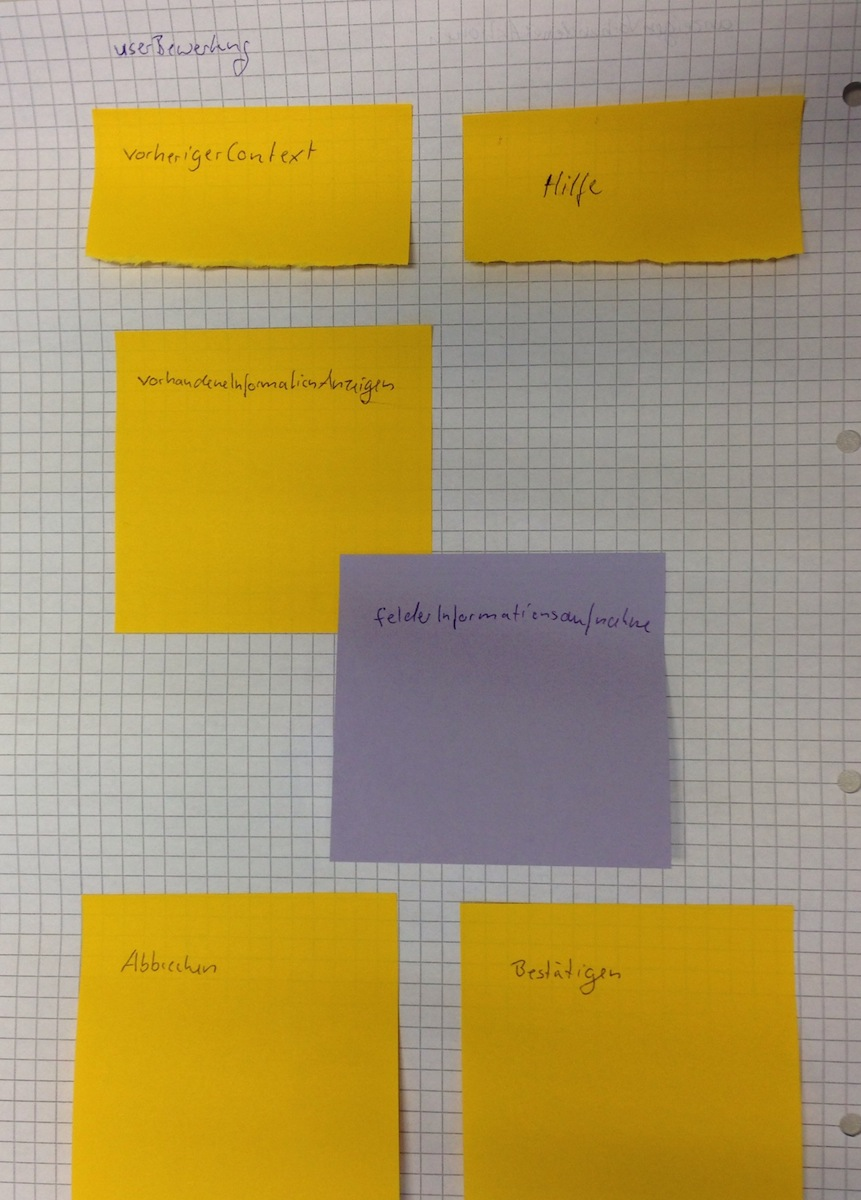
\includegraphics[angle=90, width=0.85\textwidth] {./images/abstract/version2/userBewertung.JPG}
\caption{Interaction Context AP2: userBewertung}
\label{interfaceContents50}
\end{figure}

\begin{figure}[H]
\centering
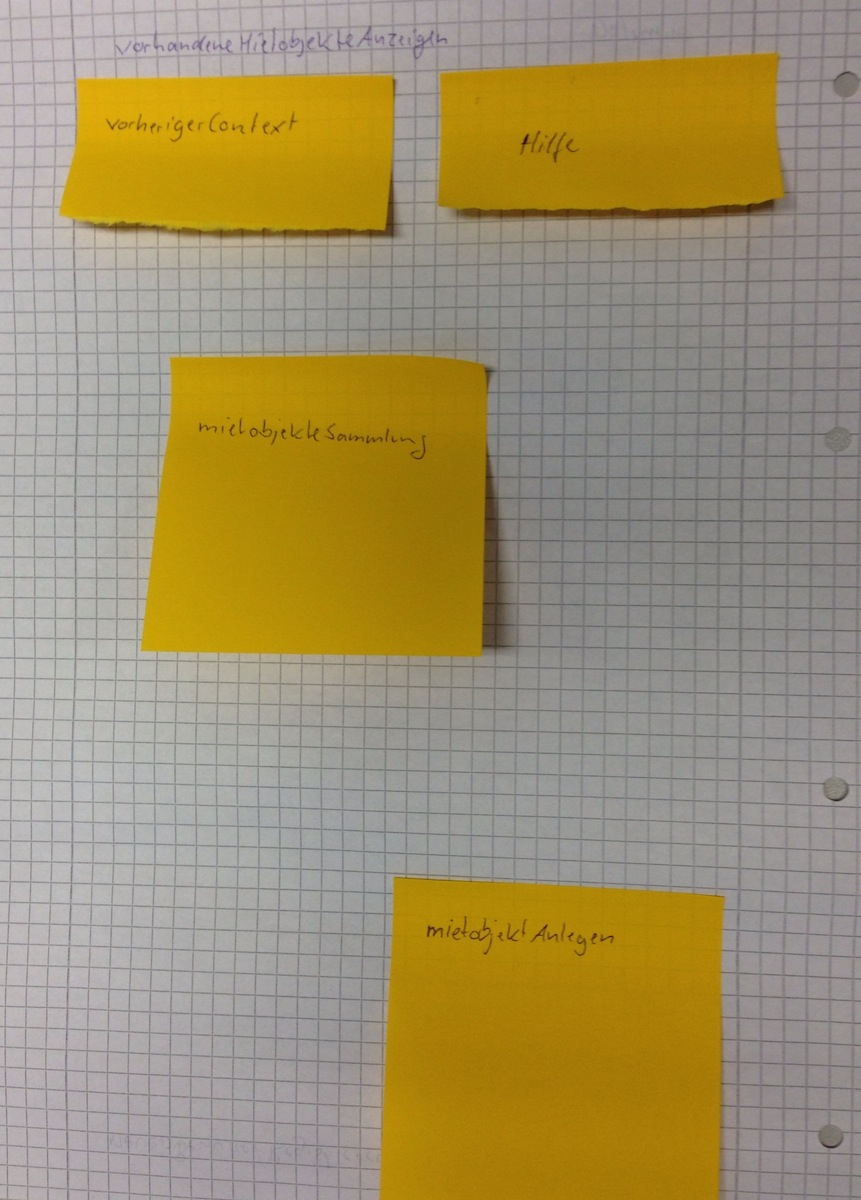
\includegraphics[angle=90, width=0.85\textwidth]  {./images/abstract/version2/vorhandeneMietobjekteAnzeigen.JPG}
\caption{Interaction Context AP2: vorhandeneMietobjekteAnzeigen}
\label{interfaceContents51}
\end{figure}


%Seite 7
\begin{figure}[H]
\centering
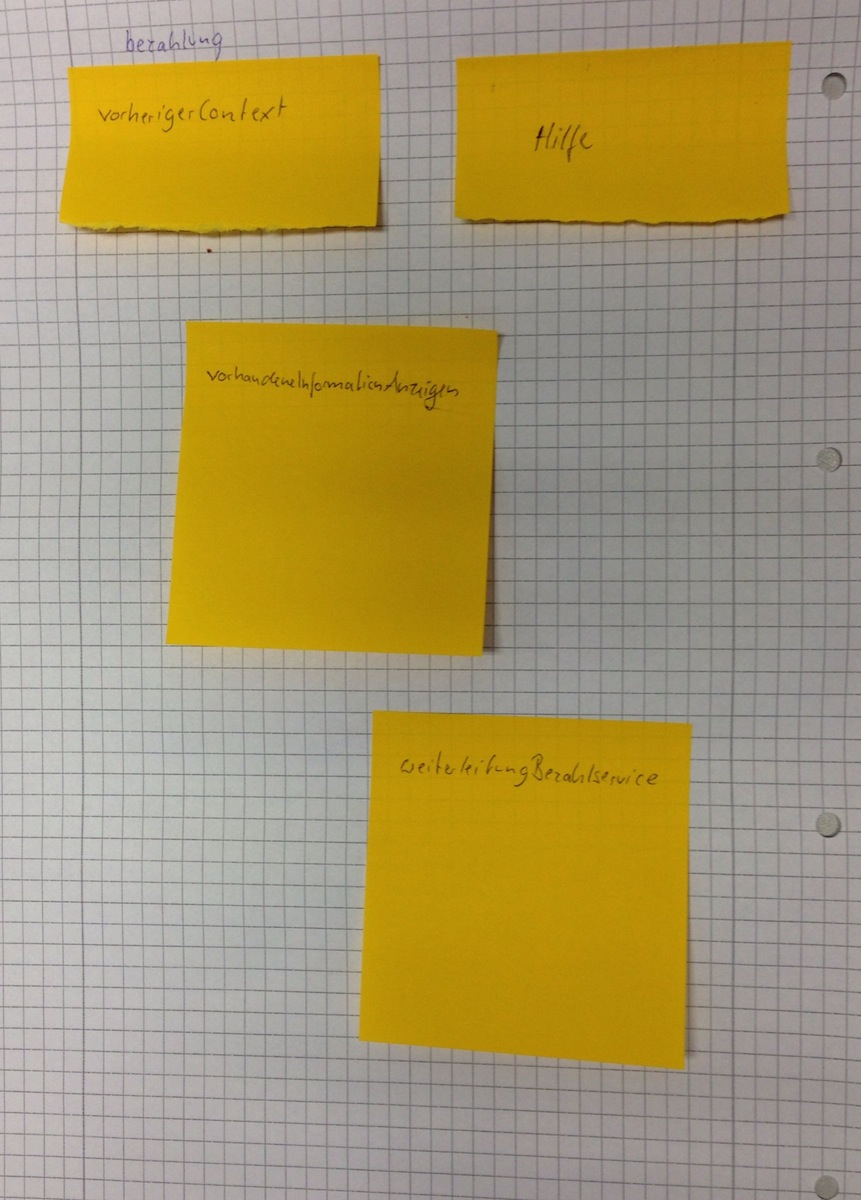
\includegraphics[angle=90, width=0.85\textwidth] {./images/abstract/version2/bezahlung.JPG}
\caption{Interaction Context AP2: bezahlung}
\label{interfaceContents52}
\end{figure}


\chapter{Paperbased Prototype 1}

\begin{figure}[H]
\centering
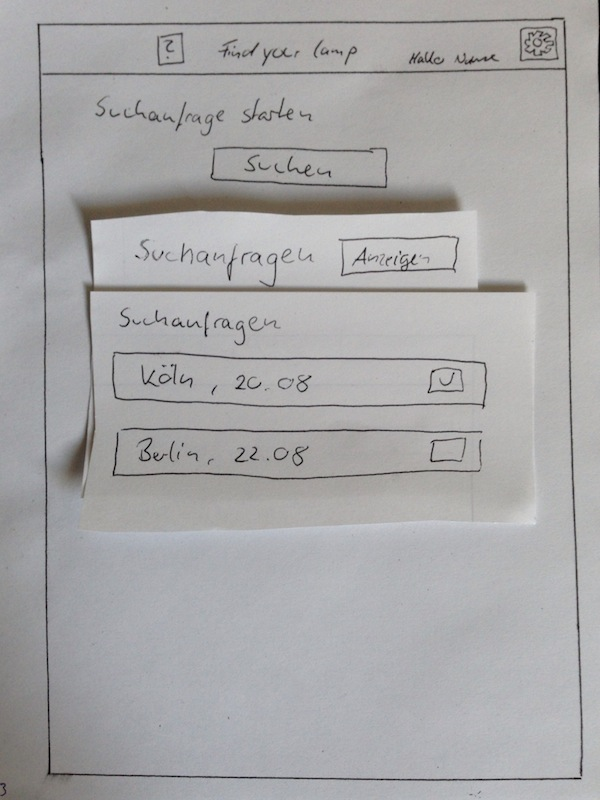
\includegraphics[angle=90, width=0.85\textwidth]{./images/paperbased/anfrage.JPG}
\caption{Pb Prototype: Übersicht der Suchanfragen}
\label{pbprototype1}
\end{figure}

\begin{figure}[H]
\centering
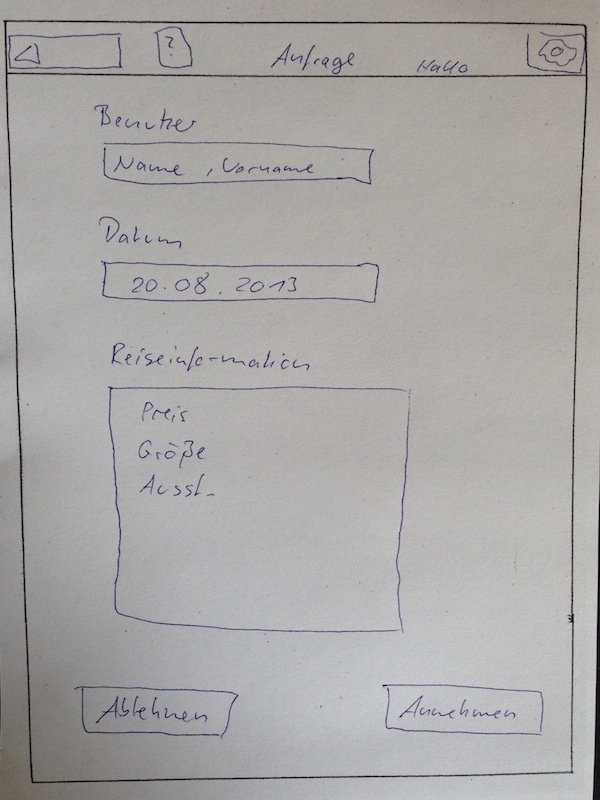
\includegraphics[angle=90, width=0.85\textwidth]{./images/paperbased/anfrageAnzeigen.JPG}
\caption{Pb Prototype: Neue Mietanfrage anzeigen}
\label{pbprototype2}
\end{figure}

\begin{figure}[H]
\centering
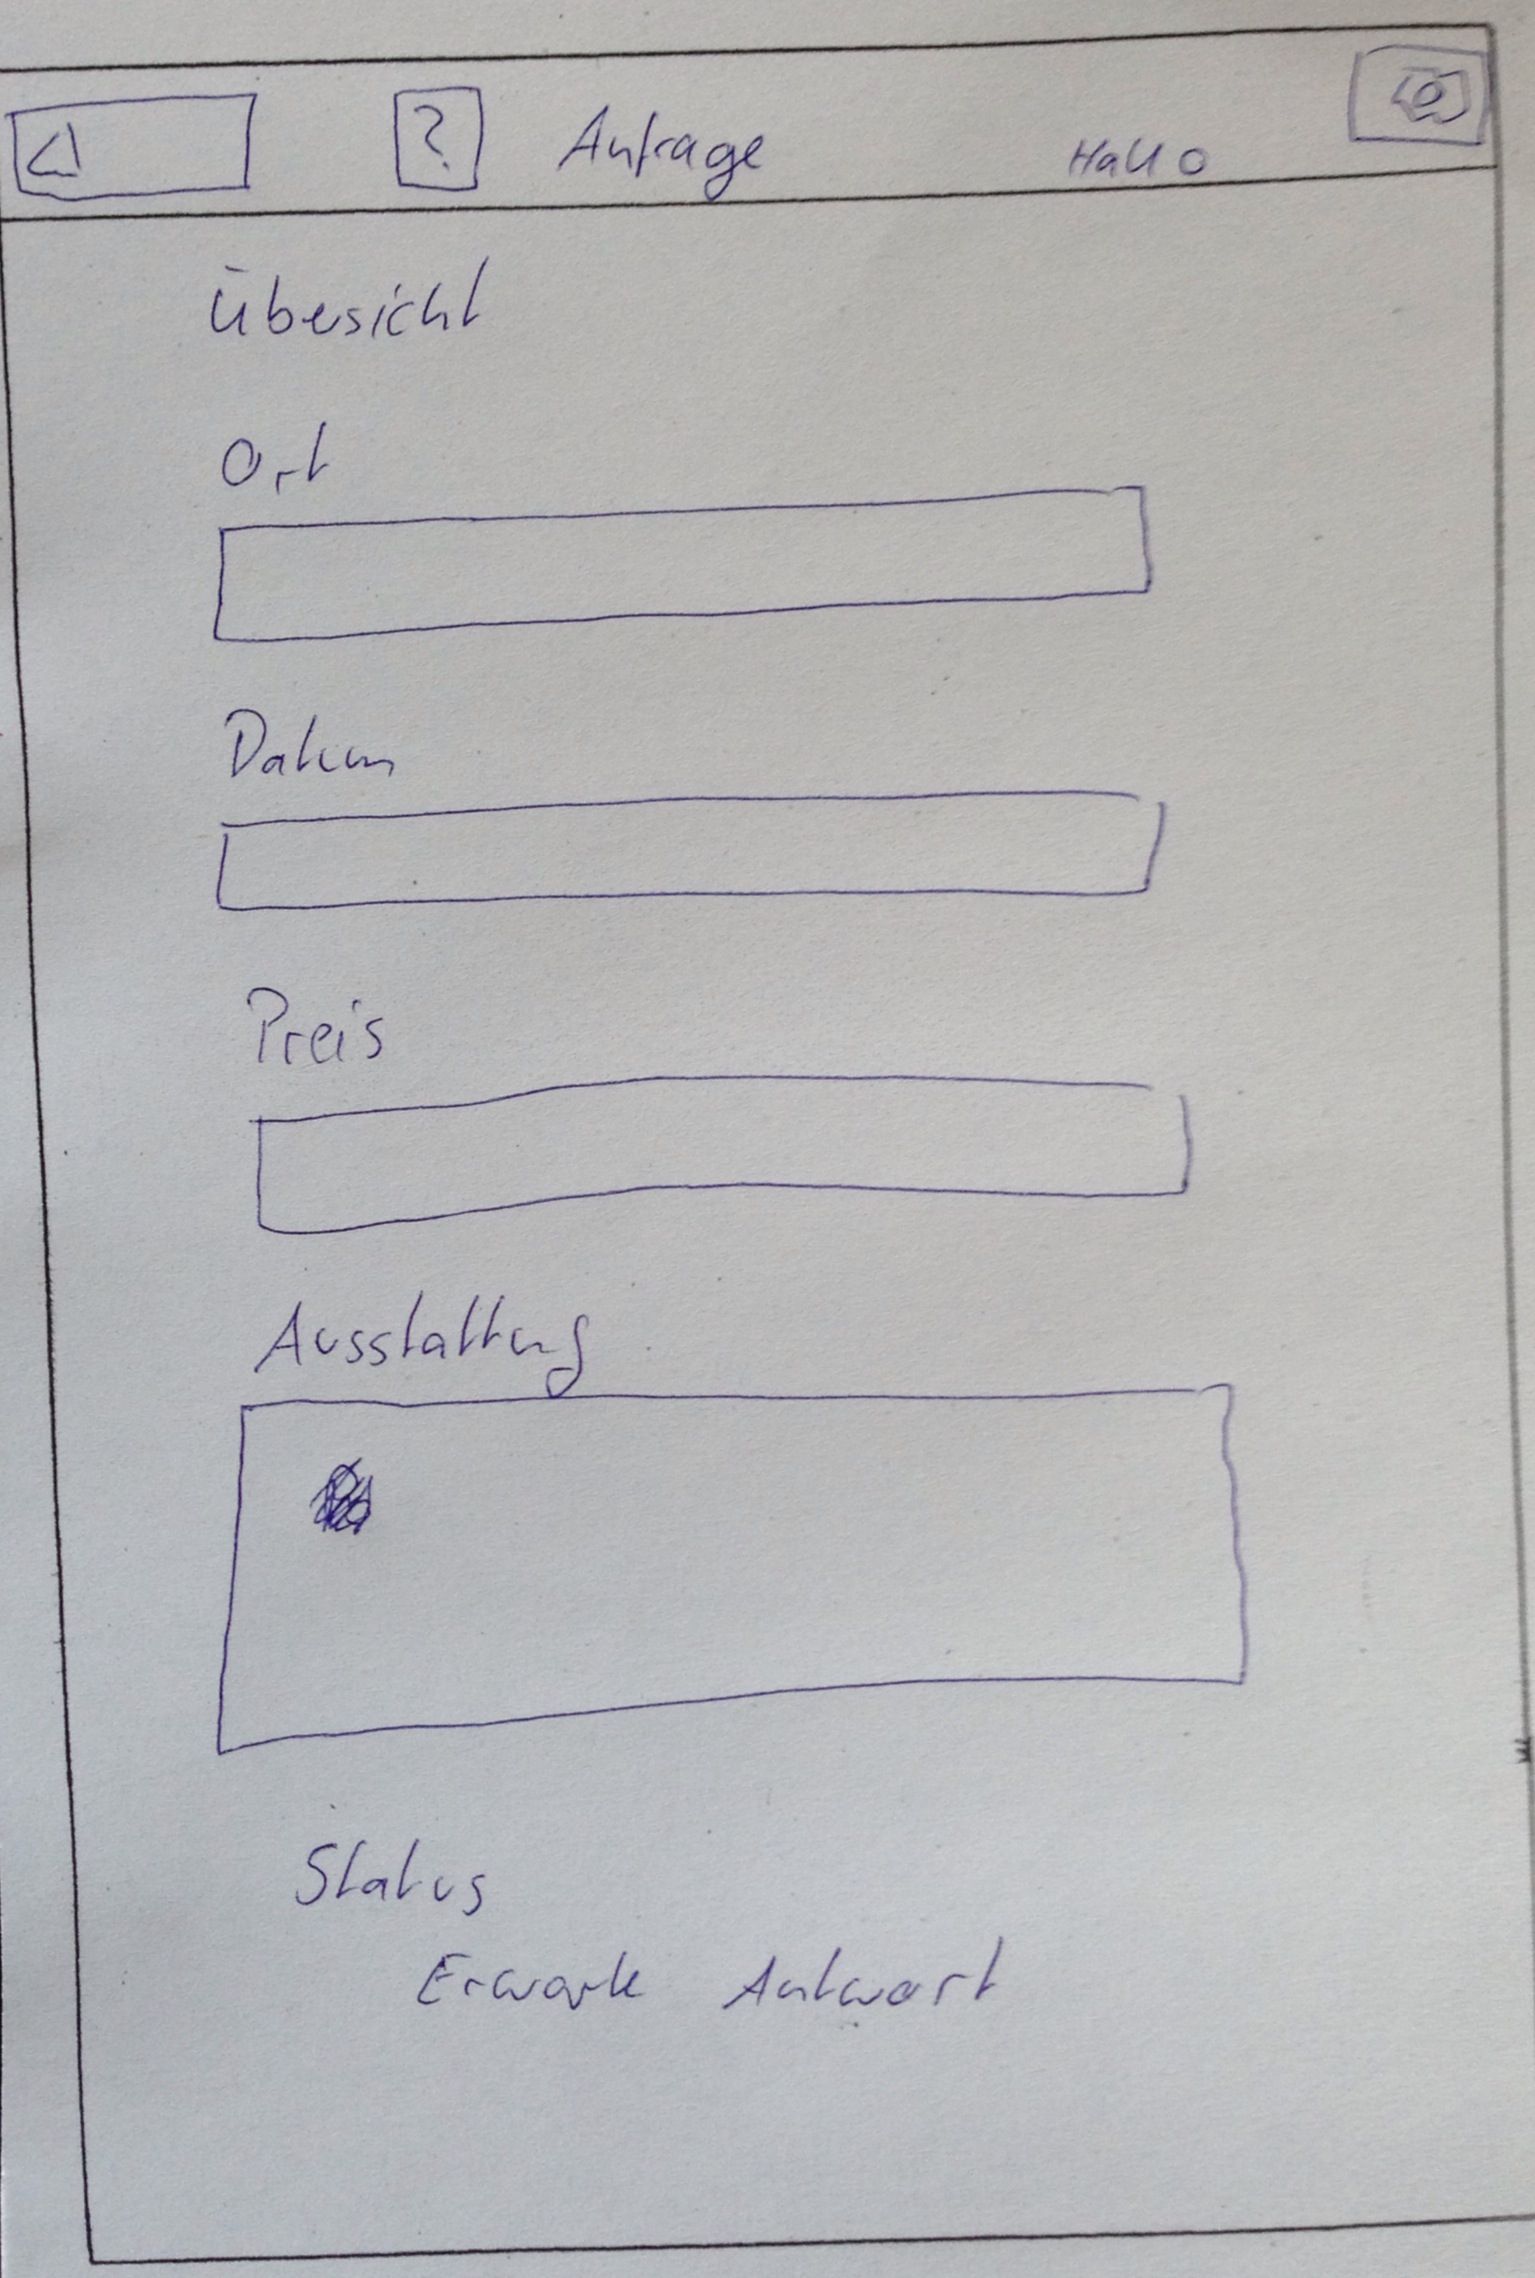
\includegraphics[angle=90, width=0.85\textwidth]{./images/paperbased/anfrageuebersicht.JPG}
\caption{Pb Prototype: Übersicht der Mietanfrage}
\label{pbprototype3}
\end{figure}

\begin{figure}[H]
\centering
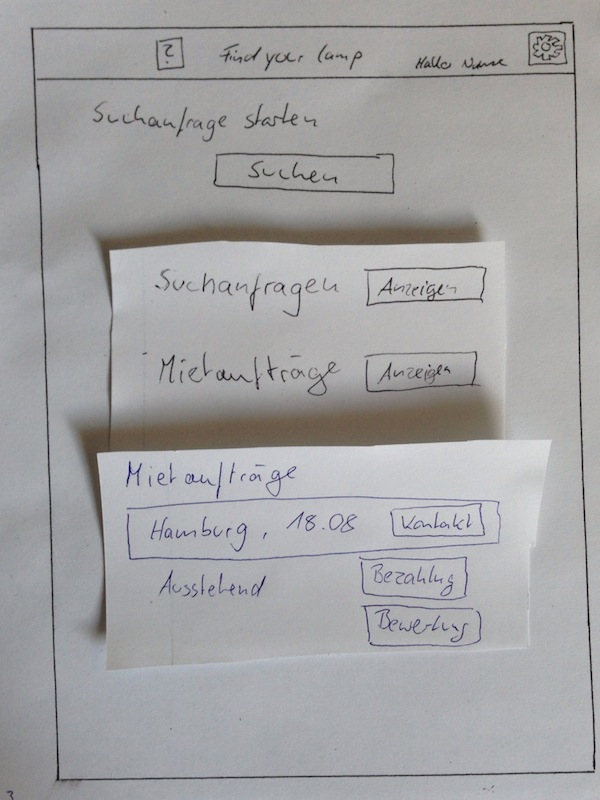
\includegraphics[angle=90, width=0.85\textwidth]{./images/paperbased/auftraege.JPG}
\caption{Pb Prototype: Übersicht der Aufträge}
\label{pbprototype4}
\end{figure}

\begin{figure}[H]
\centering
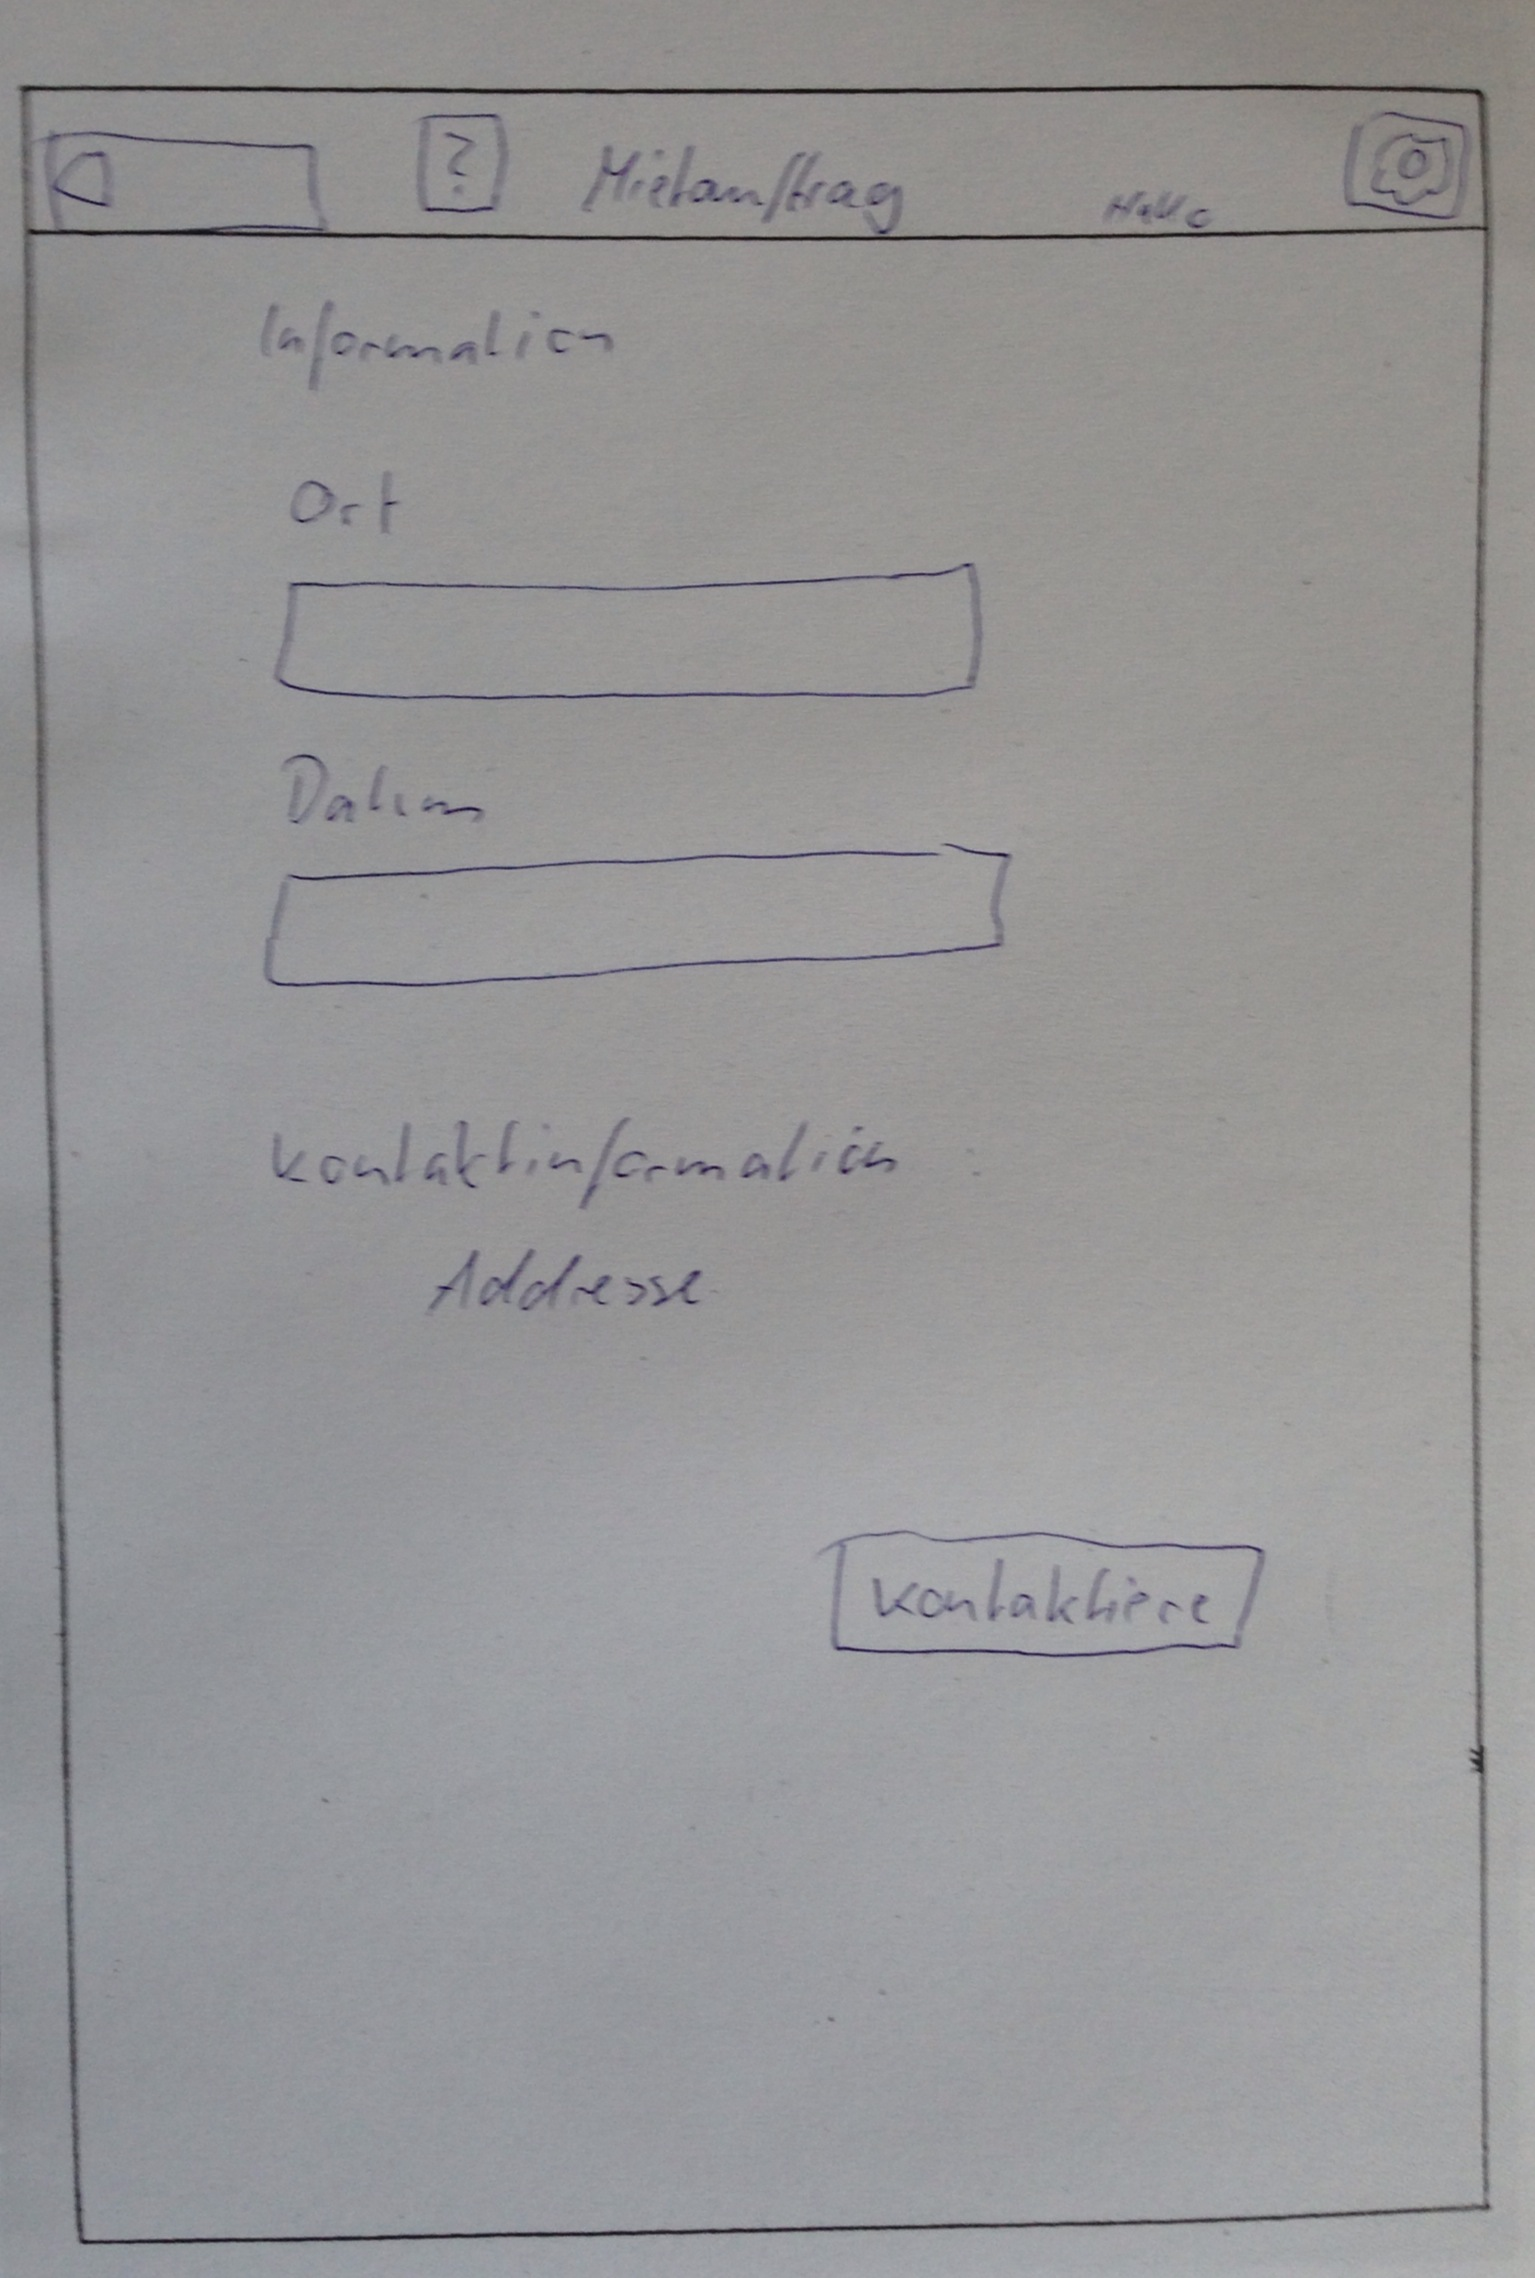
\includegraphics[angle=90, width=0.85\textwidth]{./images/paperbased/auftrag.JPG}
\caption{Pb Prototype: Übersicht eines Mietauftrags}
\label{pbprototype5}
\end{figure}

\begin{figure}[H]
\centering
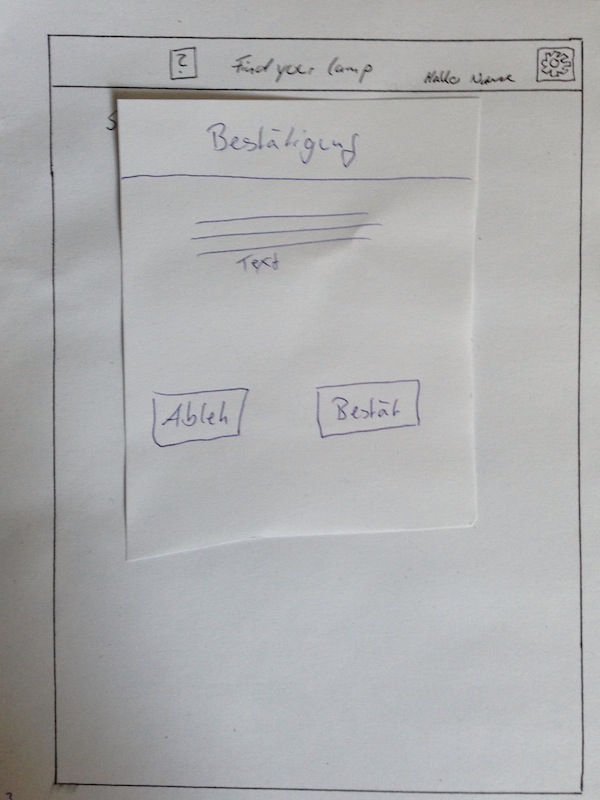
\includegraphics[angle=90, width=0.85\textwidth]{./images/paperbased/bestaetigung.JPG}
\caption{Pb Prototype: Bestätigungsnachricht}
\label{pbprototype6}
\end{figure}

\begin{figure}[H]
\centering
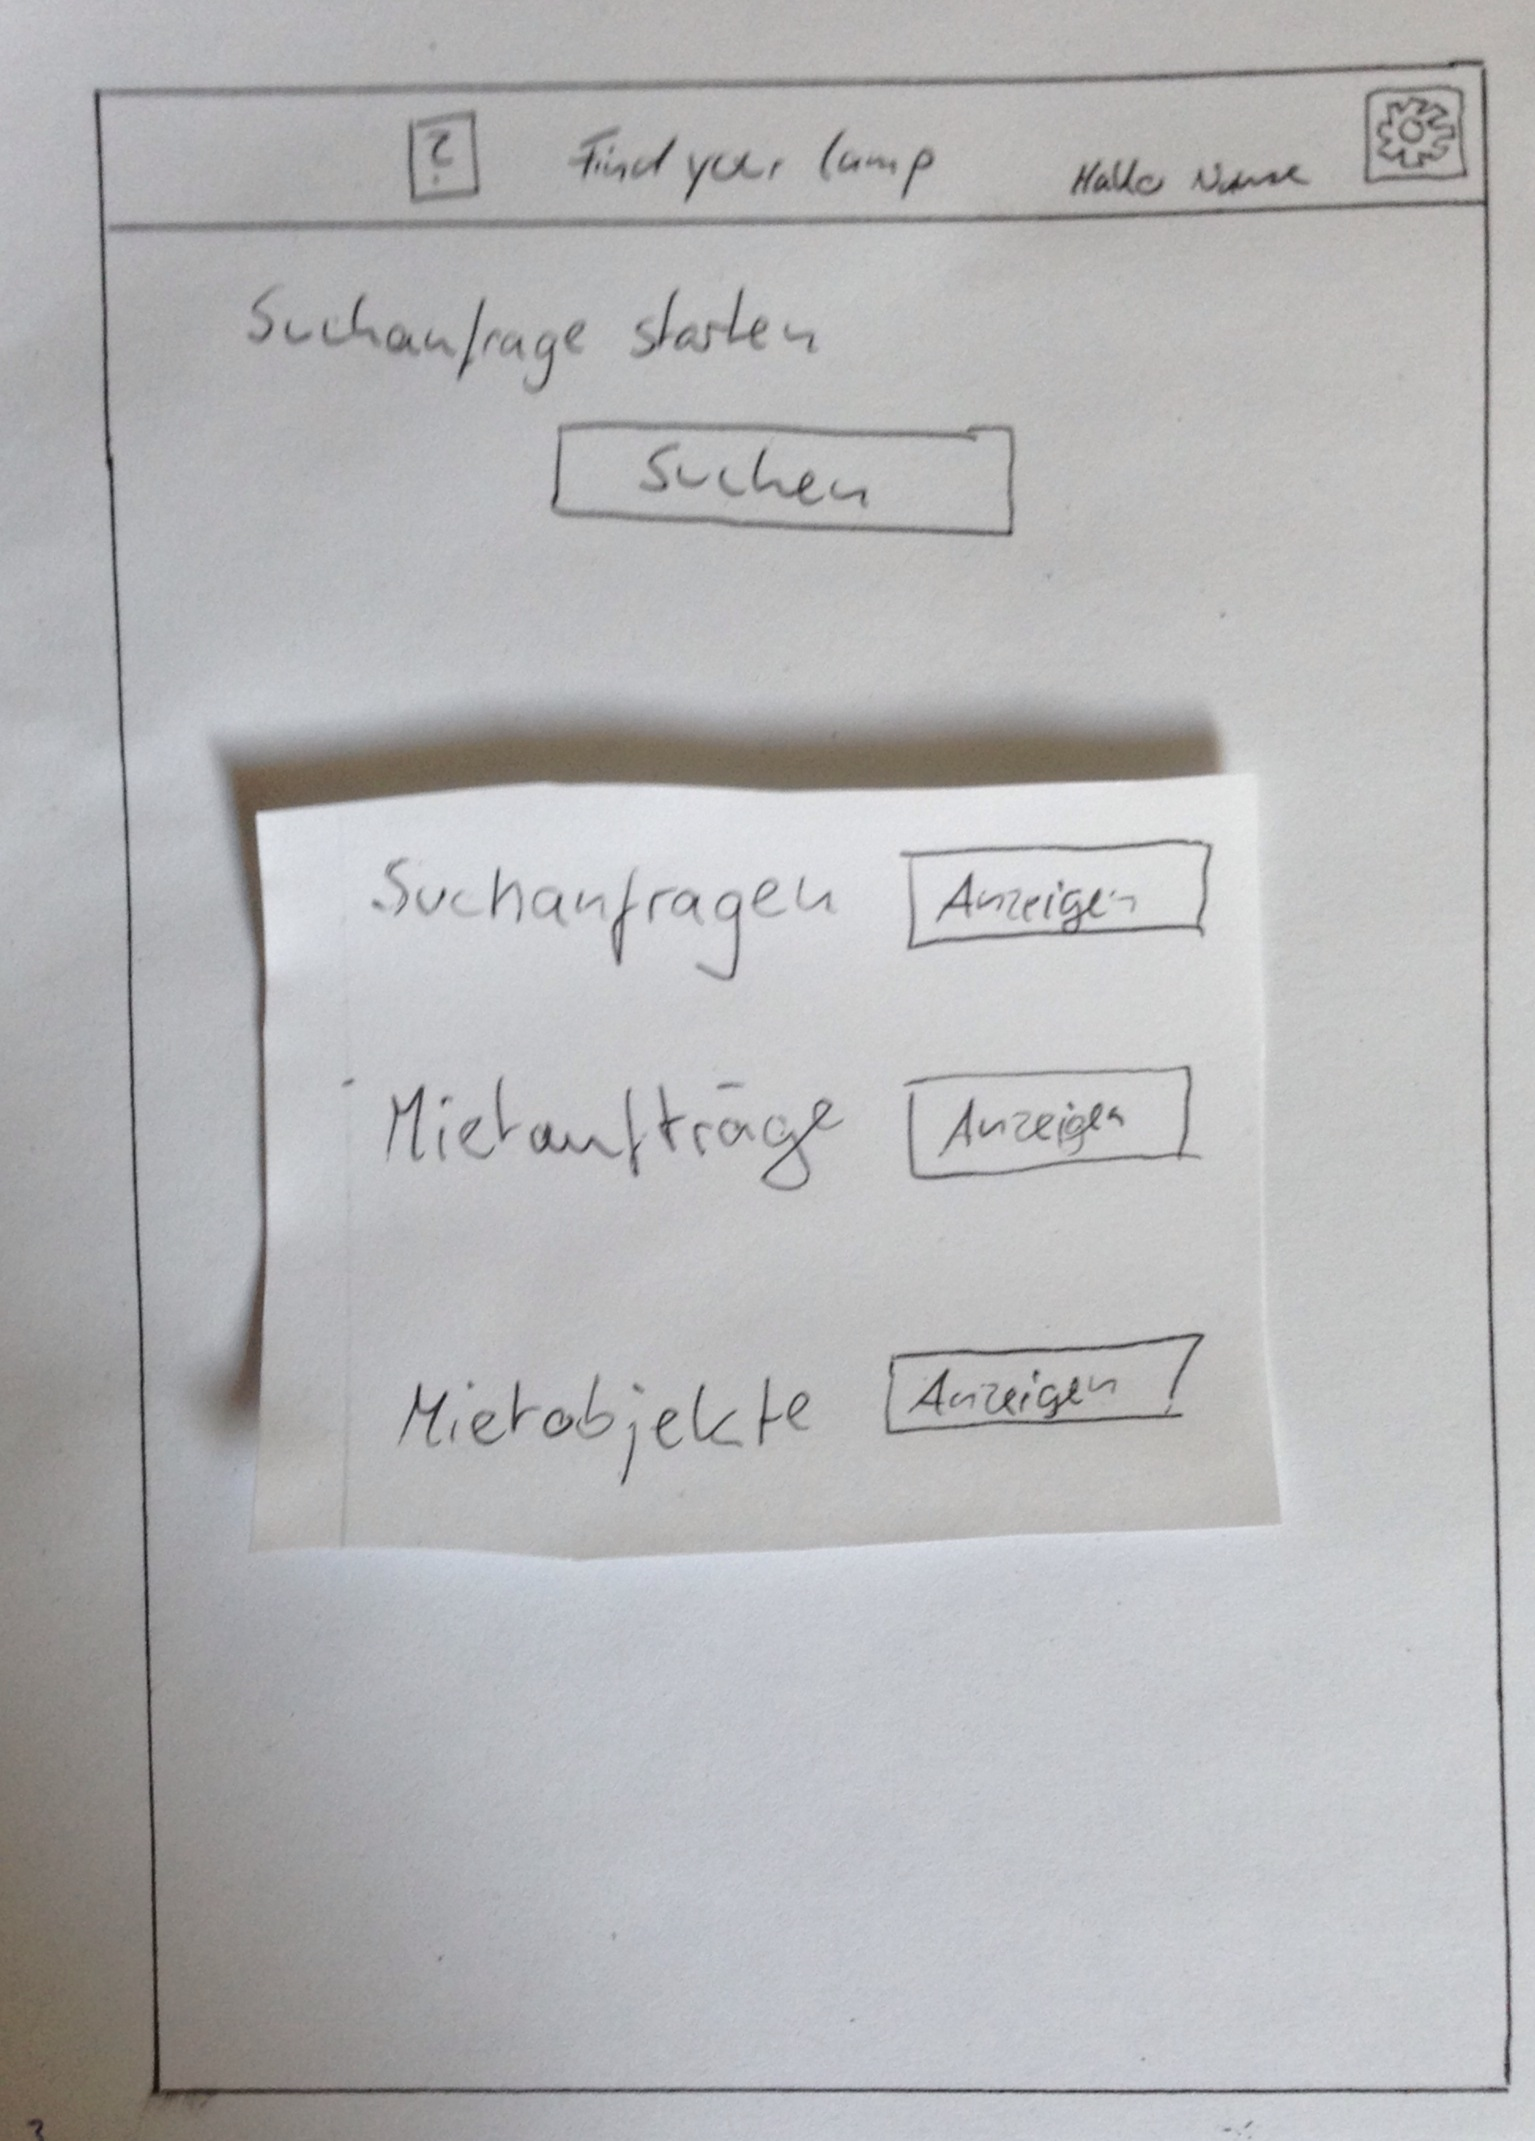
\includegraphics[angle=90, width=0.85\textwidth]{./images/paperbased/main.JPG}
\caption{Pb Prototype: Hauptscreen}
\label{pbprototype7}
\end{figure}

\begin{figure}[H]
\centering
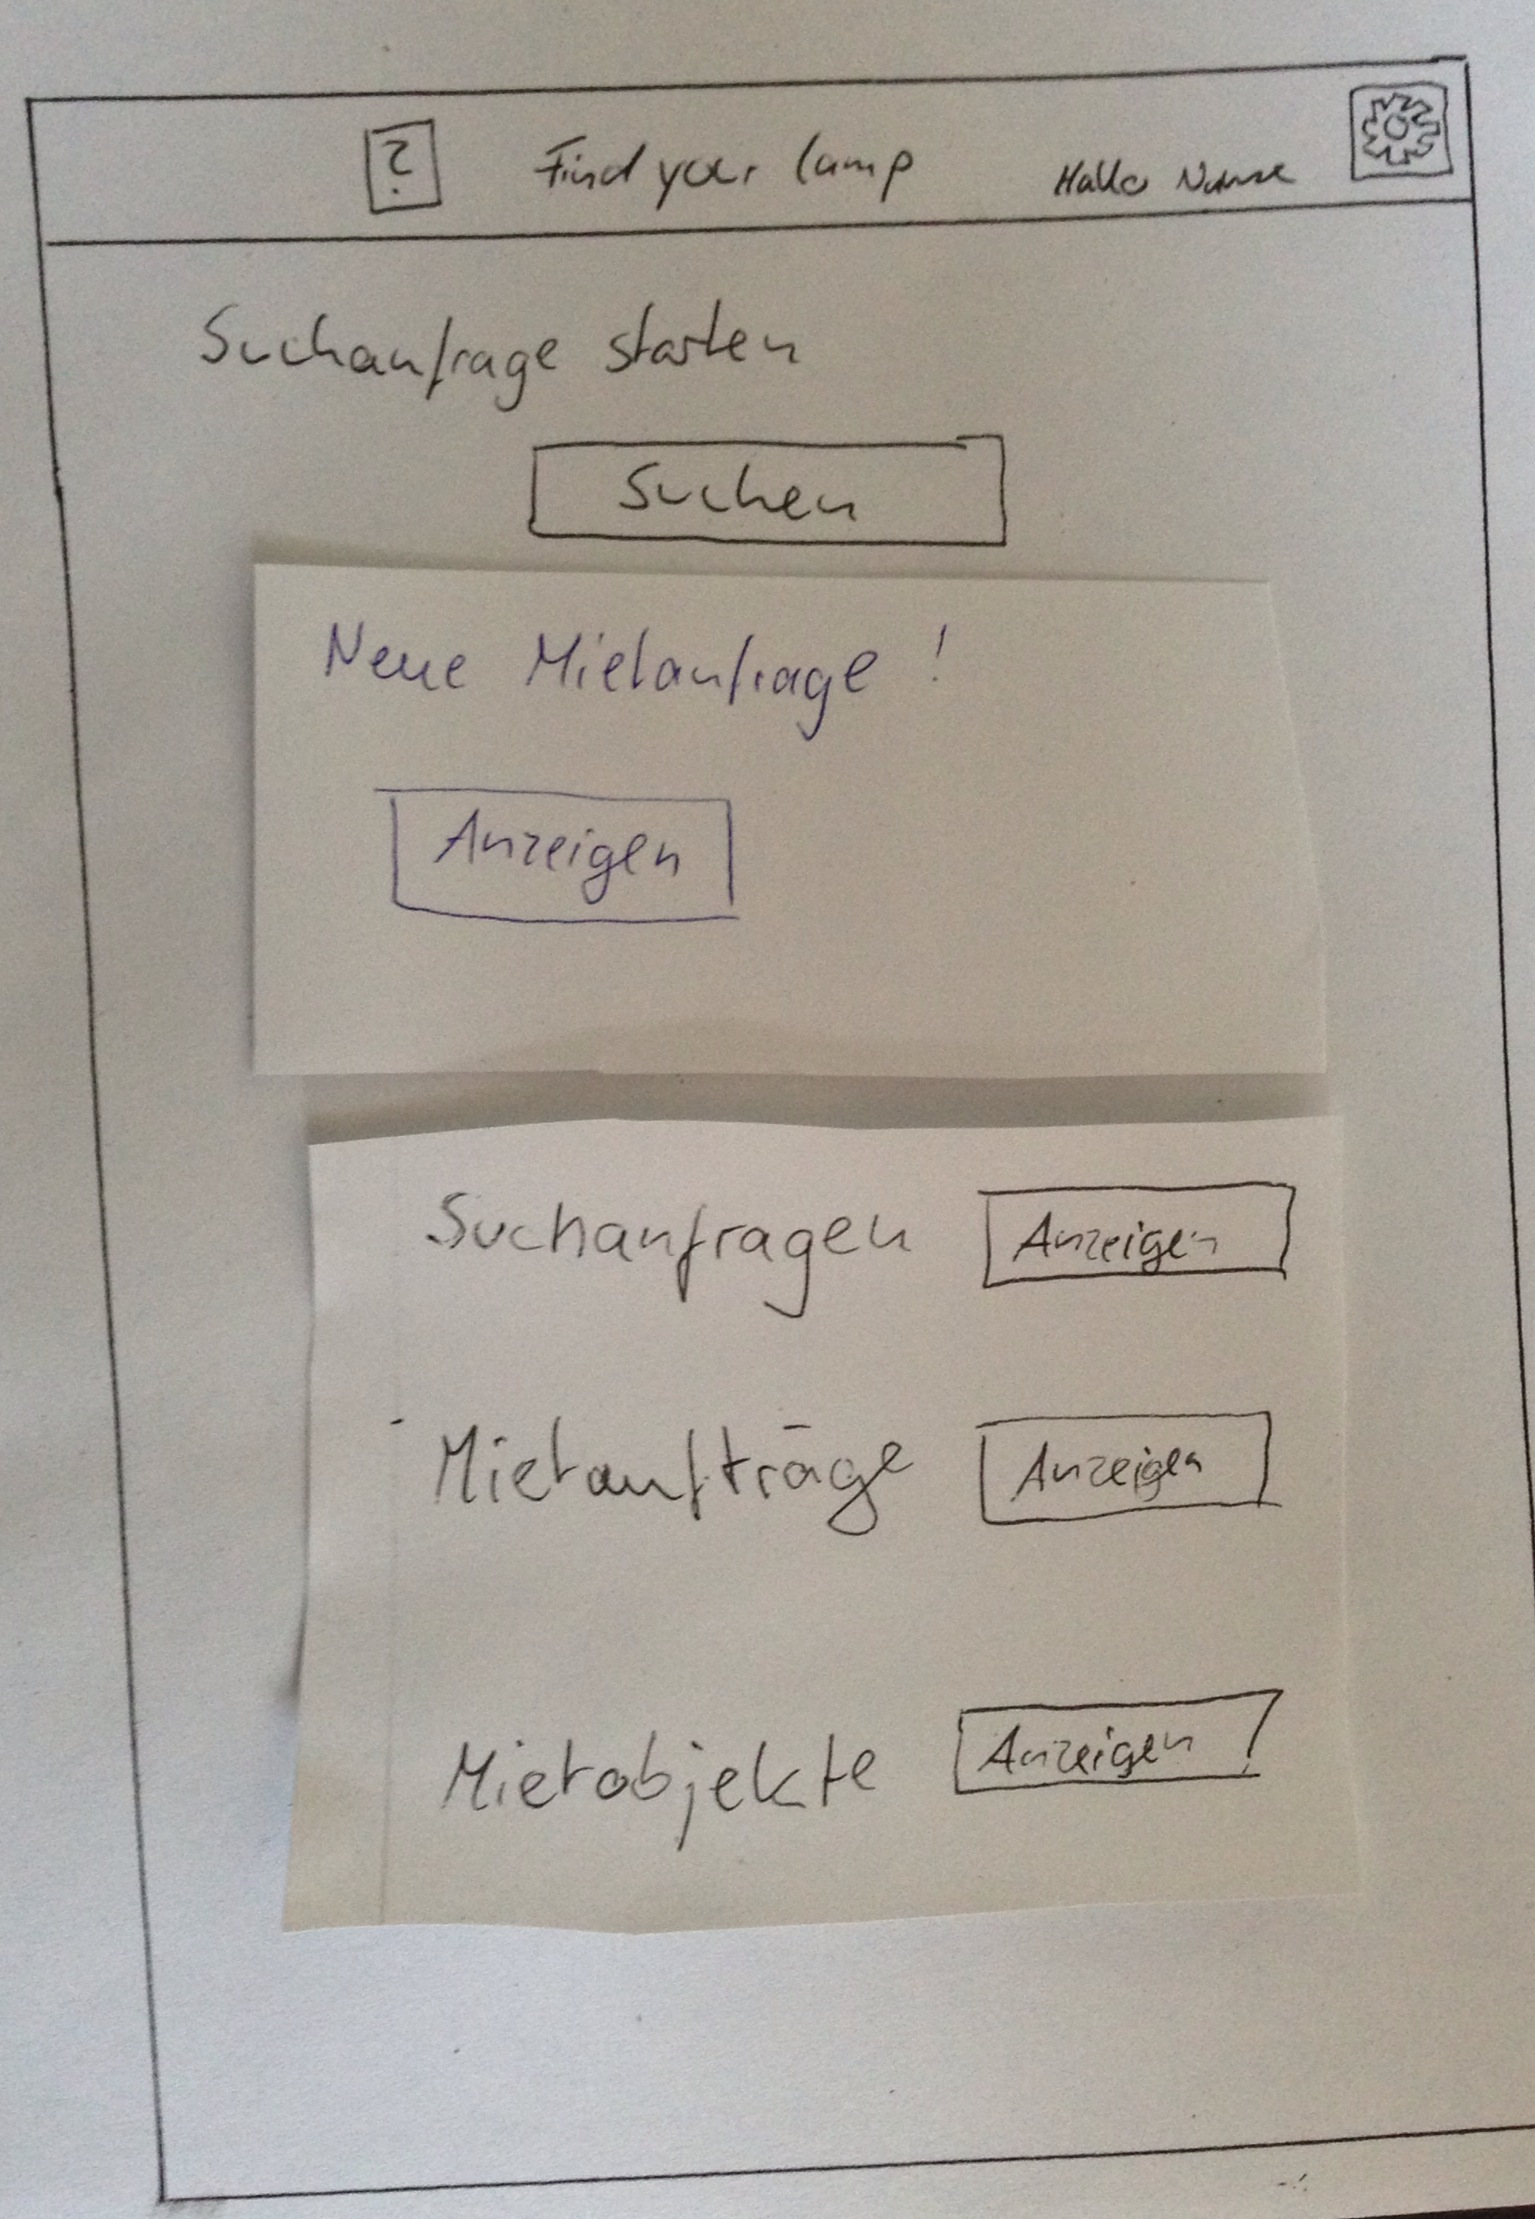
\includegraphics[angle=90, width=0.85\textwidth]{./images/paperbased/neueMietanfrage.JPG}
\caption{Pb Prototype: Mitteilung zur neuen Mietanfrage}
\label{pbprototype8}
\end{figure}

\begin{figure}[H]
\centering
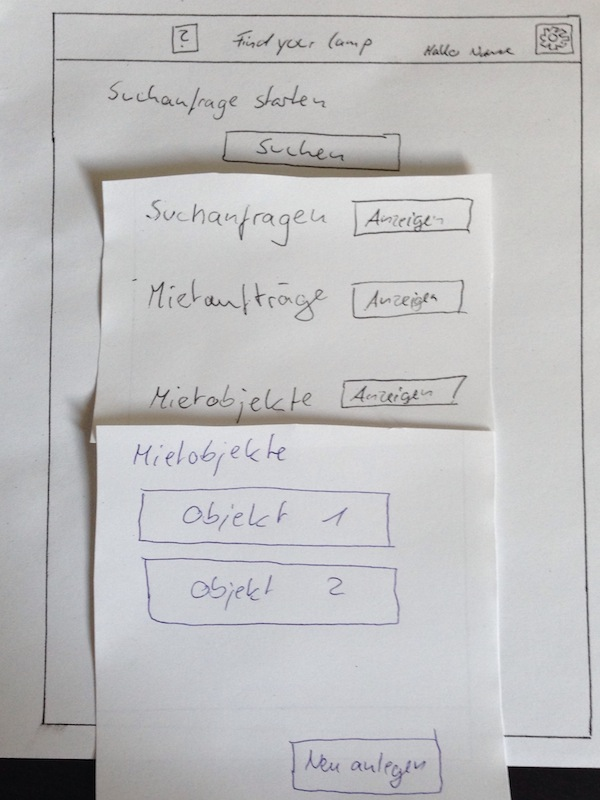
\includegraphics[angle=90, width=0.85\textwidth]{./images/paperbased/objekte.JPG}
\caption{Pb Prototype: Übersicht aller (eigenen) Mietobjekte}
\label{pbprototype9}
\end{figure}

\begin{figure}[H]
\centering
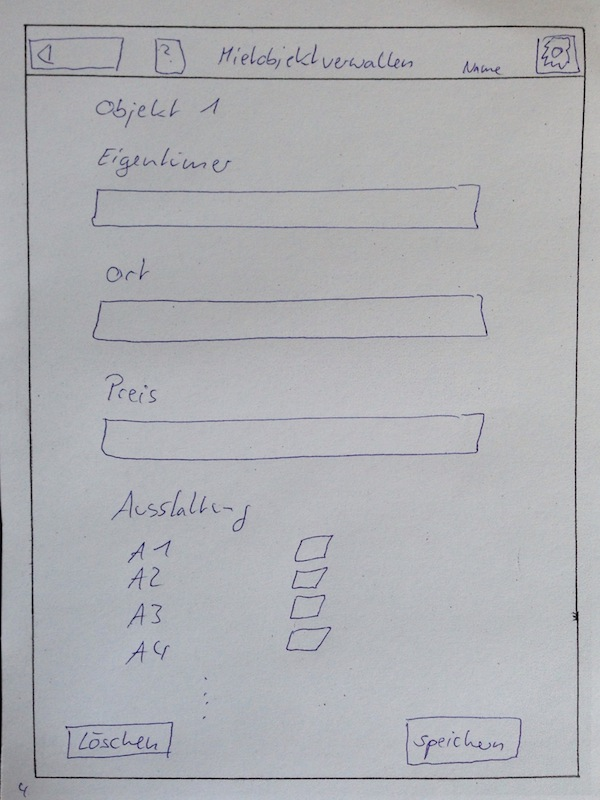
\includegraphics[angle=90, width=0.85\textwidth]{./images/paperbased/objektveralten.JPG}
\caption{Pb Prototype: Verwalten des Mietobjektes}
\label{pbprototype10}
\end{figure}

\begin{figure}[H]
\centering
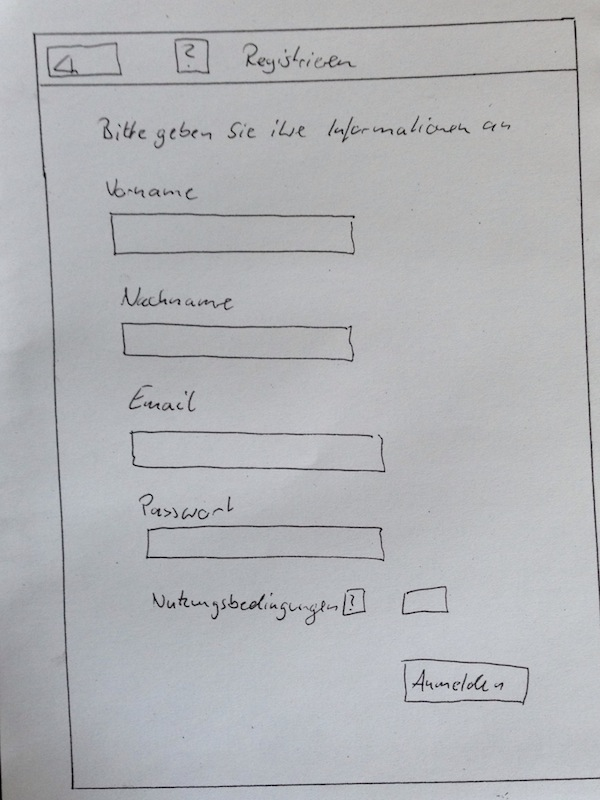
\includegraphics[angle=90, width=0.85\textwidth]{./images/paperbased/registrieren.JPG}
\caption{Pb Prototype: Registrierung}
\label{pbprototype11}
\end{figure}

\begin{figure}[H]
\centering
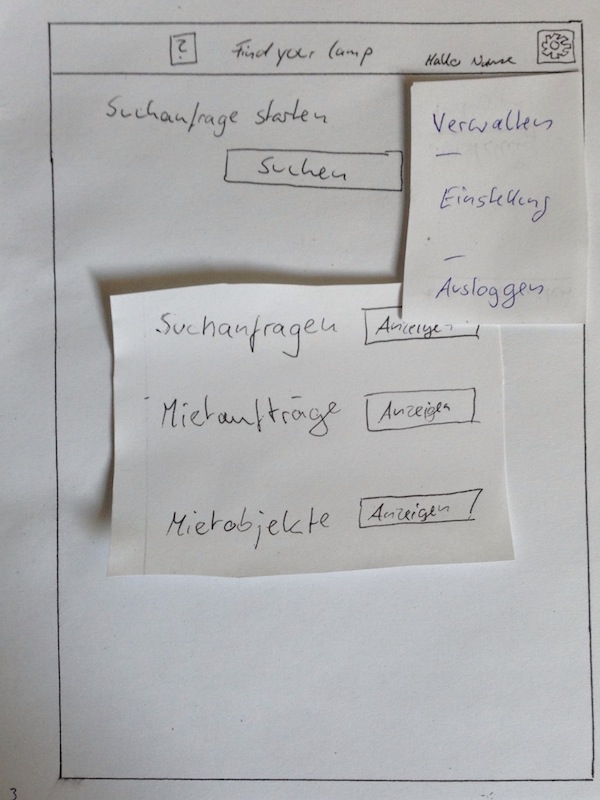
\includegraphics[angle=90, width=0.85\textwidth]{./images/paperbased/settings.JPG}
\caption{Pb Prototype: Einstellungen aktiv}
\label{pbprototype12}
\end{figure}

\begin{figure}[H]
\centering
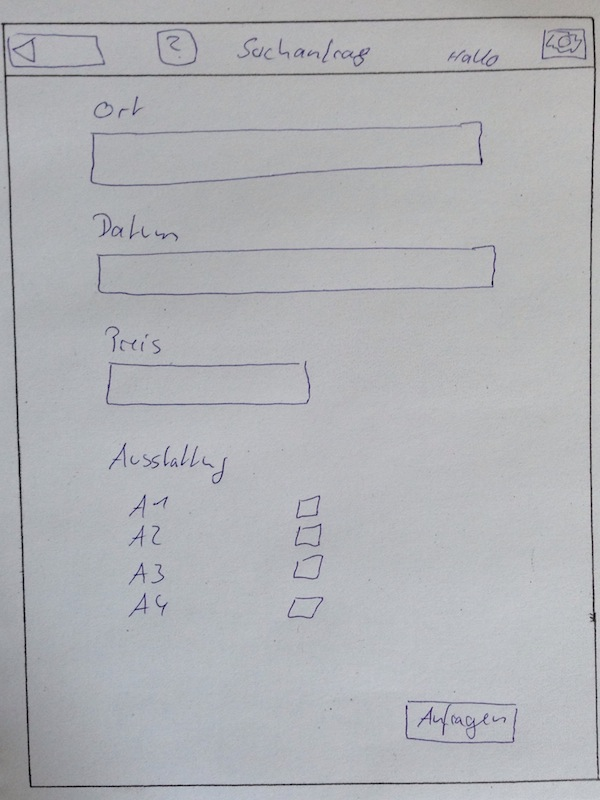
\includegraphics[angle=90, width=0.85\textwidth]{./images/paperbased/suchanfrage.JPG}
\caption{Pb Prototype: Starten einer neuen Suchanfrage}
\label{pbprototype13}
\end{figure}

\begin{figure}[H]
\centering
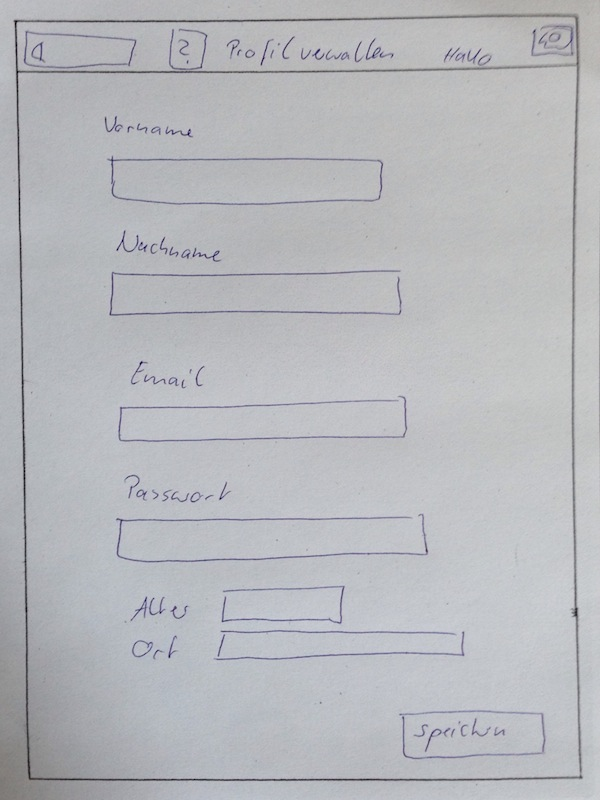
\includegraphics[angle=90, width=0.85\textwidth]{./images/paperbased/verwalten.JPG}
\caption{Pb Prototype: Verwalten des Benutzerprofils}
\label{pbprototype14}
\end{figure}

\newpage
\chapter{Projektplan}
\begin{figure}[H]
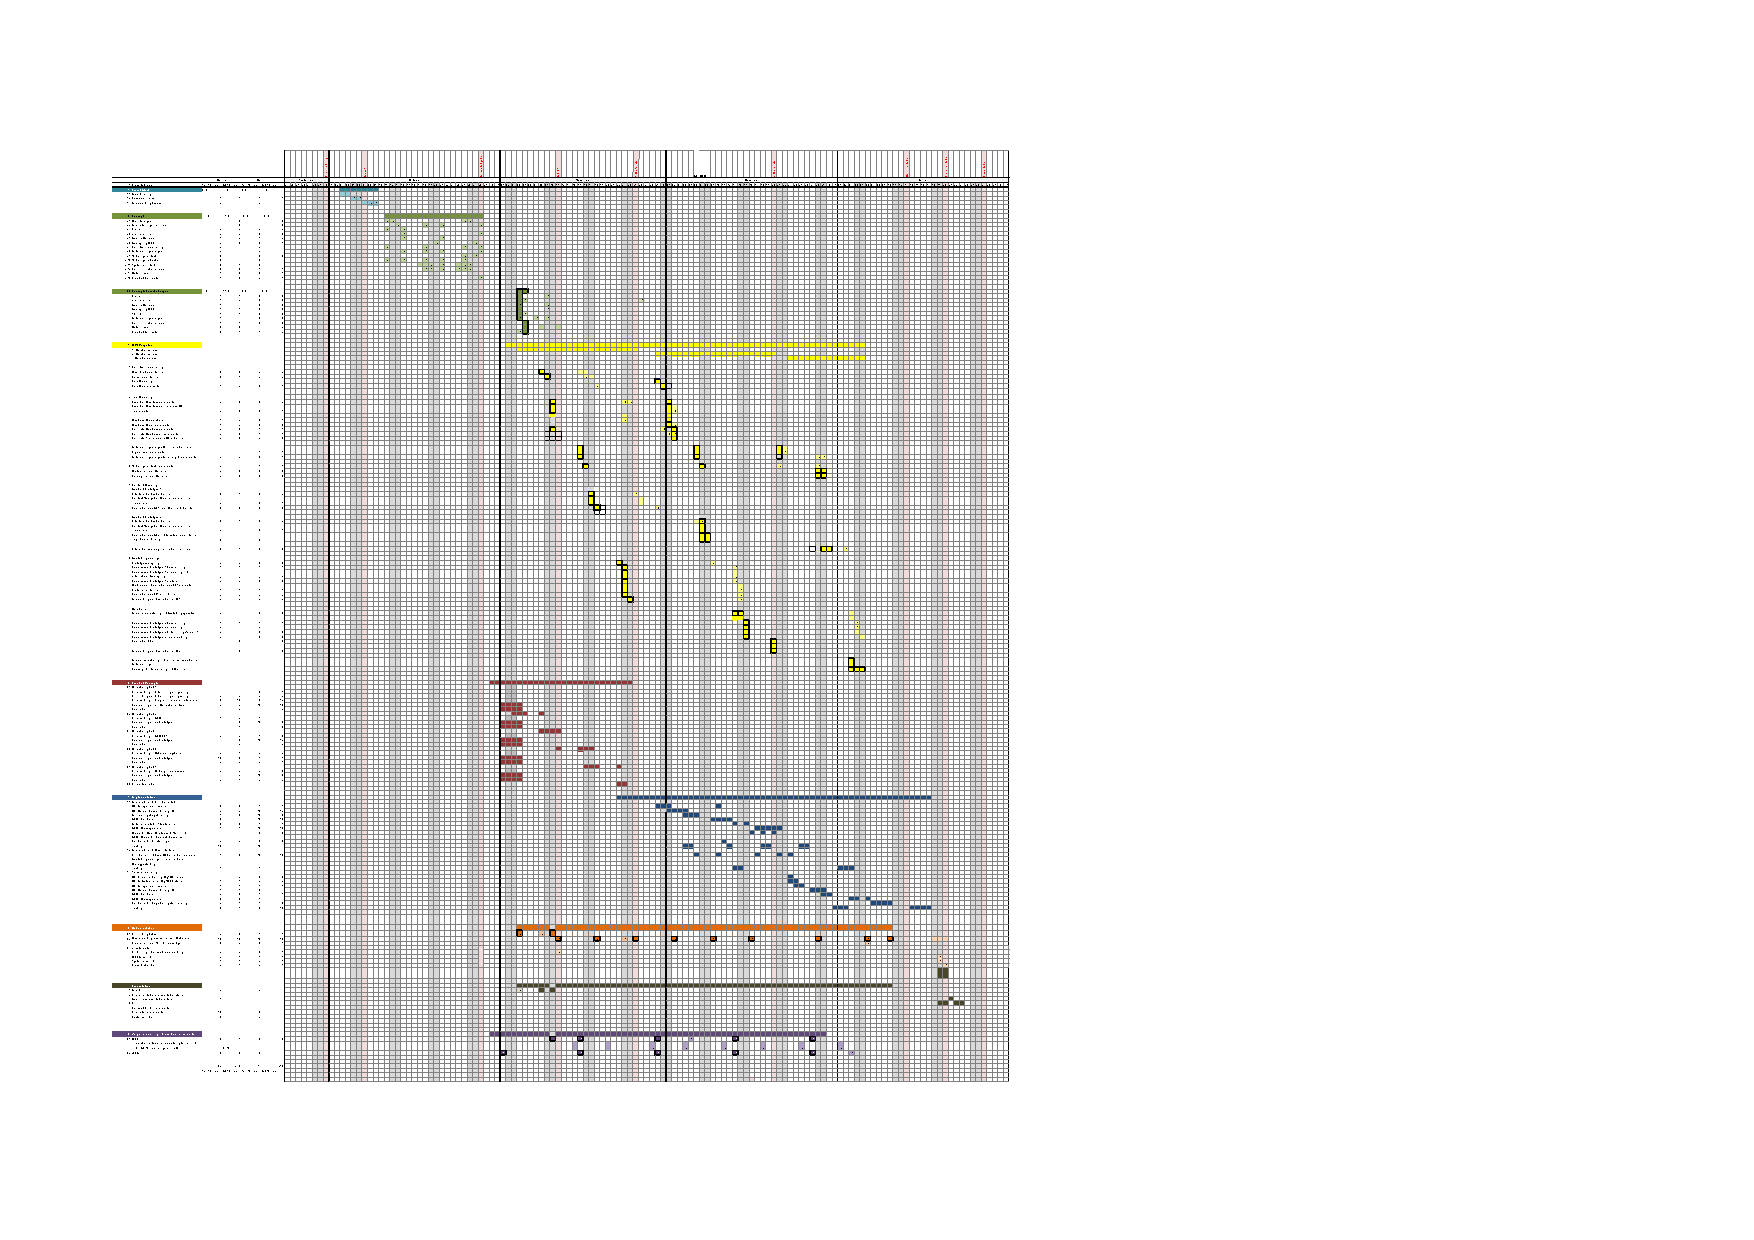
\includegraphics[width=.9\textwidth]{./images/projektplan_neu.pdf}
\caption{Projektplan}
\label{fig:projektplan}
\end{figure}

 \newpage
 %Konzeptpdf einbinden
\chapter{Konzept}
 Nachfolgend das überarbeitete Konzept.
 \includepdf[pages=1-, scale=1]{../konzept/konzept.pdf}





\end{document}
